%! Author = prat
%! Date = 14/04/2020

% Preamble
\documentclass[
    %fontsize=12pt % The default document font size, options: 10pt, 11pt, 12pt
    english, % ngerman for German
    onehalfspacing, % Single line spacing, alternatives: onehalfspacing or doublespacing
    headsepline, % Uncomment to get a line under the header
    parskip, % Uncomment to add space between paragraphs
]{MastersDoctoralThesis} % The class file specifying the document structure

\setcounter{secnumdepth}{3}

% Packages
\usepackage{lmodern}
\usepackage{scrextend}
\KOMAoption{fontsize}{12.5pt}
\usepackage[utf8]{inputenc}
\usepackage{mathtools}
\usepackage{textcomp}
\usepackage{float}
\usepackage{makeidx}
\usepackage[T1]{fontenc}
\usepackage{url}
\usepackage{todonotes}
\usepackage[all]{xy}
\usepackage{units}
\usepackage{enumerate}
\usepackage[hidelinks]{hyperref}
\usepackage[]{algorithm2e} %algorithm
\usepackage[langfont=roman,basic]{complexity}
\usepackage{amssymb, amsmath, amsthm, pict2e}
\usepackage{pdfsync}
\usepackage{rotating}
\usepackage{multirow}
\usepackage[normalem]{ulem}
\usepackage{cancel}
\usepackage{color}
\usepackage{pgf,tikz}
\usetikzlibrary{decorations.markings}
\usepackage{subcaption}
\usetikzlibrary{positioning}
\usetikzlibrary{decorations,arrows, graphs, quotes}
\usetikzlibrary{shapes.misc, positioning}
\usepgflibrary{decorations.pathreplacing}
\usetikzlibrary{arrows.meta}
\usetikzlibrary{arrows,automata}
\usepackage{pgfplots}


\def\arr{\hbox{𝓇}}
\usepackage{environ}
\usepackage{csquotes}
\usepackage{amsmath}
\usepackage{natbib}
\makeatletter
\newsavebox{\measure@tikzpicture}
\NewEnviron{scaletikzpicturetowidth}[1]{%
    \def\tikz@width{#1}%
    \def\tikzscale{1}\begin{lrbox}{\measure@tikzpicture}%
                         \BODY
    \end{lrbox}%
    \pgfmathparse{#1/\wd\measure@tikzpicture}%
    \edef\tikzscale{\pgfmathresult}%
    \BODY
}
\def\ver{0.12} %size of a vertex

\tikzset{middlearrow/.style={
    decoration={markings,
    mark= at position 0.6 with {\arrow[scale=5]{#1}} ,
    },
    postaction={decorate}
}
}

\tikzset{Bullet/.style={fill=black,draw,color=#1,circle,minimum size=2pt,scale=0.9}}


%%%%%%%%%%%%%%%%  start macros  %%%%%%%%%%%%%%%%%%%%%%%%%%%%%%%%%
\let\emph\relax
\DeclareTextFontCommand{\emph}{\bfseries\em}
\newtheorem{theorem}{Theorem}
\theoremstyle{definition}
\newtheorem{defn}[theorem]{Definition}
\newtheorem{example}[theorem]{Example}
\theoremstyle{remark}
\newtheorem{remark}[theorem]{Remark}
\newtheorem{question}[theorem]{Question}
\theoremstyle{plain}
\newtheorem{lemma}[theorem]{Lemma}
\newtheorem{claim}[theorem]{Claim}
\newtheorem{obs}[theorem]{Observation}
\newtheorem{prop}[theorem]{Proposition}
\newtheorem{corollary}[theorem]{Corollary}
\newtheorem{conjecture}[theorem]{Conjecture}
\newtheorem{hyp}[theorem]{Hypothesis}
\newtheorem{alg}[theorem]{Algorithm}
\numberwithin{theorem}{section}
\newtheorem{proofpart}{Part}
\DeclarePairedDelimiter\ceil{\lceil}{\rceil}
\DeclarePairedDelimiter\floor{\lfloor}{\rfloor}

%%%%%%%%%%%%%%%%  end macros  %%%%%%%%%%%%%%%%%%%%%%%%%%%%%%%%%

%----------------------------------------------------------------------------------------
%	MARGIN SETTINGS
%----------------------------------------------------------------------------------------

\geometry{
    paper=a4paper, % Change to letterpaper for US letter
    inner=2.5cm, % Inner margin
    outer=3.8cm, % Outer margin
    bindingoffset=.5cm, % Binding offset
    top=1.5cm, % Top margin
    bottom=1.5cm, % Bottom margin
%showframe, % Uncomment to show how the type block is set on the page
}
%----------------------------------------------------------------------------------------
%	THESIS INFORMATION
%----------------------------------------------------------------------------------------

\thesistitle{Reconfiguration Problems} % Your thesis title, this is used in the title and abstract, print it elsewhere with \ttitle
\supervisor{Dr. Jean \textsc{Cardinal}} % Your supervisor's name, this is used in the title page, print it elsewhere with \supname
\examiner{} % Your examiner's name, this is not currently used anywhere in the template, print it elsewhere with \examname
\degree{} % Your degree name, this is used in the title page and abstract, print it elsewhere with \degreename
\author{Prateeba \textsc{Ruggoo}} % Your name, this is used in the title page and abstract, print it elsewhere with \authorname
\addresses{} % Your address, this is not currently used anywhere in the template, print it elsewhere with \addressname

\subject{PSPACE COMPLETE Problems} % Your subject area, this is not currently used anywhere in the template, print it elsewhere with \subjectname
\keywords{} % Keywords for your thesis, this is not currently used anywhere in the template, print it elsewhere with \keywordnames
\university{\href{https://www.ulb.be}{Université libre de Bruxelles}} % Your university's name and URL, this is used in the title page and abstract, print it elsewhere with \univname
\department{\href{https://www2.ulb.ac.be/facs/sciences/info}{Department of Computer Science}} % Your department's name and URL, this is used in the title page and abstract, print it elsewhere with \deptname
\group{\href{http://researchgroup.university.com}{}} % Your research group's name and URL, this is used in the title page, print it elsewhere with \groupname
\faculty{\href{http://faculty.university.com}{}} % Your faculty's name and URL, this is used in the title page and abstract, print it elsewhere with \facname

\AtBeginDocument{
    \hypersetup{pdftitle=\ttitle} % Set the PDF's title to your title
    \hypersetup{pdfauthor=\authorname} % Set the PDF's author to your name
    \hypersetup{pdfkeywords=\keywordnames} % Set the PDF's keywords to your keywords
}

% Document
\begin{document}
    \newcommand{\Depth}{2}
    \newcommand{\Height}{2}
    \newcommand{\Width}{2}
    \frontmatter % Use roman page numbering style (i, ii, iii, iv...) for the pre-content pages
    \pagestyle{plain} % Default to the plain heading style until the thesis style is called for the body content

%----------------------------------------------------------------------------------------
%	TITLE PAGE
%----------------------------------------------------------------------------------------

    \begin{titlepage}
        \begin{center}

            \vspace*{.06\textheight}
            {\scshape\LARGE \univname\par}\vspace{1.5cm} % University name
            \textsc{\Large Master Thesis}\\[0.5cm] % Thesis type

            \HRule \\[0.4cm] % Horizontal line
            {\huge \bfseries \ttitle\par}\vspace{0.4cm} % Thesis title
            \HRule \\[1.5cm] % Horizontal line

            \begin{minipage}[t]{0.4\textwidth}
                \begin{flushleft} \large
                \emph{Author:}\\
                \href{}{\authorname} % Author name - remove the \href bracket to remove the link
                \end{flushleft}
            \end{minipage}
            \begin{minipage}[t]{0.4\textwidth}
                \begin{flushright} \large
                \emph{Supervisor:} \\
                \href{}{\supname} % Supervisor name - remove the \href bracket to remove the link
                \end{flushright}
            \end{minipage}\\[3cm]

            \vfill
            \groupname  \deptname  % Research group name and department name

            \vfill

            {\large \today}\\[4cm] % Date
            %\includegraphics{Logo} % University/department logo - uncomment to place it

            \vfill
        \end{center}
    \end{titlepage}

%----------------------------------------------------------------------------------------
%	QUOTATION PAGE
%----------------------------------------------------------------------------------------

    \vspace*{0.2\textheight}

    \noindent\enquote{\itshape Understand well as I may, my comprehension can only be an infinitesimal fraction of all I want to understand.}\bigbreak

    \hfill Ada Lovelace

%----------------------------------------------------------------------------------------
%	ABSTRACT PAGE
%----------------------------------------------------------------------------------------

    \begin{abstract}
        \addchaptertocentry{\abstractname} % Add the abstract to the table of contents
        Reconfiguration problems arise when we wish to find a step-by-step transformation between two feasible solutions of a problem
        such that all intermediate results are also feasible \cite{DBLP:journals/tcs/ItoDHPSUU11}. Recently, study about the solution space of
        reconfiguration problems defined as \textit{reconfiguration graph} sparked great interest. In this work, we focus on the structural questions
        (Is the reconfiguration graph connected?, Is there a path between a node $s$ and a node $t$ in the reconfiguration graph?).
        In the first half this thesis we analyse various aspects of the Constraint Logic framework, from the book “Games, Puzzles and Computation”
        by Hearn and Demaine which provides several problems that are often a convenient starting point for reductions in order to prove
        $\PSPACE$-hardness and present an in-depth study of the alternative formulation of NCL, the SLIDING TOKENS problem.
        In the second half of this thesis, we analyse the complexity results around the Boolean Satisfiability reconfiguration problems and
        focus on complementing some recent $\PSPACE$-hardness proofs given in \cite{cardinal_reconfiguration_2018} concerning the
        $k$-move SUBSET SUM RECONFIGURATION problem.


    \end{abstract}

%----------------------------------------------------------------------------------------
%	ACKNOWLEDGEMENTS
%----------------------------------------------------------------------------------------

    \begin{acknowledgements}
        \addchaptertocentry{\acknowledgementname} % Add the acknowledgements to the table of contents
        First and foremost, my utmost gratitude to Prof. Jean Cardinal, whose patience and encouragement I will never forget.
        And whose door was always open whenever I had questions concerning my research or whenever I was lost, I could always
        count on him for guidance. He consistently allowed me to be creative but steered me in the right direction whenever
        he thought I needed it.

        I am also deeply indebted to my parents who have given me the opportunity of an education and support throughout my life.
        Finally, I must express my very profound gratitude to my partner for providing me with continuous encouragement
        and a sounding board when required. This accomplishment would not have been possible without them. Thank you.

        %I would like to thank my little kitten, Koi ni who brings me everyday joy \ldots
    \end{acknowledgements}

%----------------------------------------------------------------------------------------
%	LIST OF CONTENTS/FIGURES/TABLES PAGES
%----------------------------------------------------------------------------------------
    \hypersetup{linkcolor=black}
    \tableofcontents % Prints the main table of contents

%\listoffigures % Prints the list of figures

%\listoftables % Prints the list of tables

%----------------------------------------------------------------------------------------
%	DEDICATION
%----------------------------------------------------------------------------------------

    \dedicatory{Every challenging work needs self efforts as well as
                the support of those who are very close to our heart.
                My humble effort I dedicate to my sweet and loving


                Family $\&$ Partner


                Whose love, affection and encouragement made me able to
                complete this challenge,

                Along with all hard working and respected


                Teachers}

%----------------------------------------------------------------------------------------
%	THESIS CONTENT - CHAPTERSFor/Dedicated to/To my\ldots
%----------------------------------------------------------------------------------------

    \mainmatter % Begin numeric (1,2,3...) page numbering

    \pagestyle{thesis} % Return the page headers back to the "thesis" style

% Include the chapters of the thesis as separate files from the Chapters folder
\chapter{Introduction}\label{ch:intro}
Reconfiguration problems are computational problems in which we wish to find a step-by-step transformation between two feasible solutions
(referred as configurations) of a problem such that all intermediate results are also feasible. A configuration can be the arrangement of puzzle
pieces, the ordering of symbols to form a string or the location of a robot with respect to obstacles in space. Combinatorial reconfiguration
problems ask the reachability between the two given satisfying solutions. The area of reconfiguration considers both structural and algorithmic
problems on the space of solutions, under various definitions of feasibility and adjacency.


The \textit{reconfiguration framework} is defined in terms of a source problem, an instance of the source problem, a definition of a feasible solution
and a definition of adjacency of feasible solutions. Viewing reconfiguration problems from a graph-theoretic perspective, the notion of a
\textit{reconfiguration graph} naturally arises. Let $G$ be a reconfiguration graph where the vertex set consists of all
possible configurations and two nodes are connected by an edge if the corresponding configurations can each be obtained from the other by the
application of a single transformation rule,\textit{a reconfiguration step}. Any path or walk in the reconfiguration graph corresponds to a
sequence of reconfiguration steps called a \textit{reconfiguration sequence}.

Interest in combinatorial reconfiguration begun with the Sliding blocks puzzles and steadily increased during the last decade. The reconfiguration framework has recently been applied in a number of settings,
including vertex colouring \cite{bonsma}, \cite{bonsma_cereceda}, \cite{cereceda}, list-edge colouring \cite{ito_reconfiguration_2009}, clique, set cover,
integer programming, matching, spanning tree, matroid bases \cite{DBLP:journals/tcs/ItoDHPSUU11}, block puzzles \cite{hearn_pspace-completeness_2004},
shortest path \cite{shortest_path}, independent set \cite{hearn_pspace-completeness_2004},\cite{DBLP:journals/tcs/ItoDHPSUU11}, \cite{kaminski_complexity_2012},
and satisfiability \cite{DBLP:journals/siamcomp/GopalanKMP09}.
Many problems in $\P$ have their reconfiguration problems in $\P$ as well, such as spanning tree, matching, and matroid problems in general. On the other hand,
the reconfigurability of independent set, set cover, and integer programming are $\PSPACE$-complete \cite{DBLP:journals/tcs/ItoDHPSUU11}. In general however, knowing
the complexity of a decision problem does not allow us to directly infer the complexity status of its reconfiguration problem(s). Several $\NP$-complete problems have
reconfigurability analogues that are in $\P$, for example the $3$-colourability problem \cite{DBLP:conf/iwoca/JohnsonCH08}. Alternatively, some problems in $\P$
have reconfigurability versions that are $\PSPACE$-complete, such as shortest paths \cite{DBLP:journals/corr/abs-1009-3217} or the problem of deciding whether
two $4$-colourings of a given bipartite or planar graph are reconfigurable \cite{bonsma}.

This thesis does not attempt to catalogue all research results that can be categorized as reconfiguration, but instead focuses on demonstrating the
main themes in the area and complement some recent $\PSPACE-$hardness proofs given in \cite{cardinal_reconfiguration_2018}. More precisely, we go
over and detail the $\PSPACE-$completeness of the following decision problems :
\begin{itemize}
    \item Given two subsets of a set $S$ of integers of integers with the same sum, can one subset be transformed into the other by adding or removing
    at most 3 elements of $S$ at a time, such that the intermediate subsets also have the same sum ?
    \item In the process of complementing the $3$-move subset sum reconfiguration problem, we also give a simple hardness proof the labelled variant
    of the sliding token problem, described in section \ref{sec:labelled_sliding_token}.
\end{itemize}

In the first half of this thesis, we study the Nondeterministic Constraint Logic of Computation introduced by Hearn and Demaine.
The NCL framework consists of different graph games ($i.e.$ problems) specific for every major complexity class, more specifically the
class $\PSPACE$. These graph games are created in order to facilitate the reduction to other games. Reviewing NCL as part of this thesis is
fundamental since it has been and still is the trigger for many $\PSPACE-$ hardness results.

The second part of this thesis focuses on Satisfiability reconfiguration problems and the Subset sum reconfiguration problem and
provides a visual support for the latter problem with the intent on helping to have a better idea of the reconfiguration graph and its
connectivity properties. Finally, in Chapter 7 our conclusions are presented and some proposals for future work are made.



\chapter{Preliminaries}
\label{chap:preliminaries}
This chapter serves as a general introduction to some mathematical concepts that are of interest to us.
\section{Graph theory}

\subsection{Basic Notation}
Let $G$ be a simple, undirected graph with vertex set $V(G)$ and edge set $E(G)$. The \textit{neighborhood} of a vertex $v$ is denoted by
$N_{G}(v) = \{u | uv \in E(G)\}$. The \textit{degree} of a vertex $v \in G$, denoted by $deg_{G}(v)$, is $|N_{G}(v)|$. Then
$\Delta(G) = max_{v \in V(G)} deg_{G}(v)$ and $\delta(G) = min_{v \in V(G)} deg_{G}(v) $ is the maximum and minimum degree of $G$, respectively.
A subgraph of $G$ is a graph $G^{'}$ such that $V(G^{'}) \subseteq V(G)$ and $E(G^{'}) \subseteq E(G)$ (see Fig.~\ref{fig:subgraph}).

A \textit{walk} of length $l$ from $v_0$ to $v_l$ in $G$ is a vertex sequence $v_0, \dots ,v_{l}$, such that for all
$i \in \{0,\dots,l-1\}$, $v_{i}v_{i+1} \in E(G)$. It is a path if all vertices are distinct. A path from a vertex $u$ to a vertex $v$ is also
called a \textit{$uv-$path}. A graph $G$ is \textit{connected} if there is a path between every pair of vertices. The \textit{$k$-th power} of
a graph $G = (V,E)$ is the graph $G^{k}$ whose vertex set is $V$ and two distinct vertices $u,v$ are adjacent in $G^{k}$ if and only if the
shortest path distance between $u$ and $v$ in $G$ is at most $k$.

An \textit{independent set} of a graph $G$ is a vextex-subset of $G$ in which
no two vertices are adjacent. Given a set of elements $\{1,2,\dots,n\}$ (called the universe, denoted $\mathcal{U}$) and a
collection $\mathcal{S}$ of $m$ sets whose union equals the universe, an \textit{exact cover} is a sub-collection $\mathcal{S}^{*}$ of $\mathcal{S}$
such that each element in $\mathcal{U}$ is contained in exactly one subset in $\mathcal{S}^{*}$.
For an in-depth review of general graph theoretic definitions, the reader can refer to Diestel's textbook \cite{diestel_graph_2000}.
%%%%%%%%%%%%%%%%%%%%%%%%%%%%%%%%%%%%%%%%%%%%%%%% BEGINING OF A FIGURE %%%%%%%%%%%%%%%%%%%%%%%%%%%%%%%%%%%%%%%%%%%%%%%
\begin{figure} [H]
    \centering
    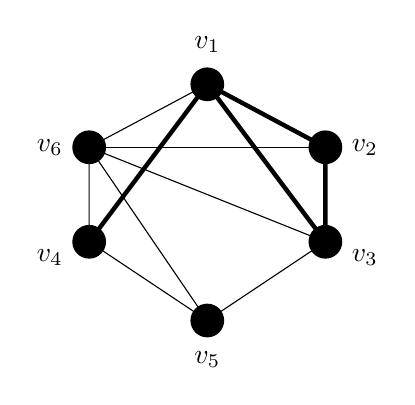
\begin{tikzpicture}
        \def\xa{1}
        \def\ya{5}
        %nodes
        \draw[thick, fill=black] (\xa,\ya) circle (0.2cm);         % v5
        \draw[thick, fill=black] (\xa+1.5,\ya+1) circle (0.2cm);   % v3
        \draw[thick, fill=black] (\xa+1.5,\ya+2.2) circle (0.2cm); % v2
        \draw[thick, fill=black] (\xa,\ya+3) circle (0.2cm);       % v1
        \draw[thick, fill=black] (\xa-1.5,\ya+2.2) circle (0.2cm); % v6
        \draw[thick, fill=black] (\xa-1.5,\ya+1) circle (0.2cm);   % v4
        %labels
        \node (1) at (\xa,\ya+3.5) {$v_1$};     % v1
        \node (2) at (\xa+2,\ya+2.2) {$v_2$};   % v2
        \node (3) at (\xa+2,\ya+0.8) {$v_3$};   % v3
        \node (5) at (\xa,\ya-0.5) {$v_5$};     % v5
        \node (4) at (\xa-2,\ya+0.8) {$v_4$};   % v4
        \node (6) at (\xa-2,\ya+2.2) {$v_6$};   % v6
        %edges
        \draw (\xa,\ya)--(\xa+1.5,\ya+1)--(\xa+1.5,\ya+2.2)--(\xa,\ya+3)--(\xa-1.5,\ya+2.2)--(\xa-1.5,\ya+1)--(\xa,\ya) ; % contour
        \draw (\xa,\ya)--(\xa-1.5,\ya+2.2) ;         % v5 - v6
        \draw (\xa+1.5,\ya+1)--(\xa-1.5,\ya+2.2) ;   % v3 - v6
        \draw (\xa+1.5,\ya+2.2)--(\xa-1.5,\ya+2.2) ; % v2 - v6
        \draw (\xa,\ya+3)--(\xa-1.5,\ya+1) ;         % v1 - v4
        \draw (\xa,\ya+3)--(\xa+1.5,\ya+1) ;         % v1 - v3
        % Hypergraph
        %edges
        \draw[ultra thick] (\xa,\ya+3)--(\xa+1.5,\ya+2.2)--(\xa+1.5,\ya+1)--(\xa,\ya+3) ; % contour
        \draw[ultra thick] (\xa,\ya+3)--(\xa-1.5,\ya+1) ;         % v1 - v4
    \end{tikzpicture}
    \caption{Graph $G^{'}$ (shown darker) is a subgraph of $G$.}
    \label{fig:subgraph}
\end{figure}
%%%%%%%%%%%%%%%%%%%%%%%%%%%%%%%%%%%%%%%%%%%%%%%% ENDING OF A FIGURE %%%%%%%%%%%%%%%%%%%%%%%%%%%%%%%%%%%%%%%%%%%%%%%

\subsection{Graph colouring}
In graph theory, a \textit{graph colouring} is a special case of \textit{graph labeling} as it is an assignment of labels traditionally
called "colours" to elements of a graph subject to certain constraints. In this work, the type of colourig that is of interest is
\textit{vertex colouring}. A \textit{proper vertex colouring} is a labeling of the graph’s vertices with colours such that no two adjacent
vertices have the same color.

A colouring using at most $k$ colours is called a \textit{(proper) $k$-colouring}.
A (proper) \textit{$k$-vertex-colouring} of a graph $G$ is a mapping $\phi$ from $V(G)$ to $\{1, 2, \dots, k\}$ (whose elements are called
\textit{colours})such that no two adjacent vertices receive the same colour, that is, $\phi(v) \neq \phi(v^{'})$ for all $v, v^{'} \in V(G)$
where $v \neq v^{'}$.
The \textit{chromatic number} of a graph $G$, denoted
$\chi{G}$, is the least number of distinct colours with which $G$ can be properly coloured. A graph that can be assigned a \textit{(proper) $k$-colouring}
is \textit{$k$-colorable}, and it is \textit{$k$-chromatic} if its chromatic number is exactly $k$. A subset of vertices assigned to the same colour
is called a \textit{colour class}, every such class forms an \textit{independent set}. Thus, a $k$-coloring is the same as a partition of the
vertex set into $k$ independent sets.


\section{Computational Complexity Theory} \label{sec:complexity}
Computer problems come in different varieties; some are easy, and some are hard. For example the sorting problem is an easy one compared to the
scheduling problem where say we have to find a schedule for the entire university to satisfy some reasonable constraints, such as that no two classes
take place in the same room at the same time. The scheduling problem seems to be much harder than the sorting problem.

In theoretical computer science, the theory of computation studies how efficiently a problem can be solved on a model of computation, using an
algorithm. A \textit{problem} or a \textit{language} is a set $L$ of strings of length at most $n$ over a finite alphabet $\Sigma$.
A \textit{decision problem} is a problem that can be posed as a YES/NO question. A string $s \in L$ is a yes instance of $L$ and a string $s \notin L$ is
a no-instance of $L$. An \textit{algorithm} is an unambiguous procedure of how to solve a class of problems.

The model of computation focused on in standard complexity theory is the \textit{Turing Machine}. It uses an unlimited tape as its unlimited memory
and has a tape head that can write and read symbols and move along the tape. A Turing Machine can be viewed as an automaton, following simple rules
to change states, with an aim to end in an accepting or a rejecting state. Two critical ressources for the Turing Machine are \textit{time} which is
the number of steps it requires to reach an accepting or a rejecting state and \textit{space} being the amount of information that needs to be
remembered throughout the computation.

A Turing Machine that can choose which moves to take in order to reach an accepting state is known as a \textit{Nondeterministic Turing Machine}
contrary to a \textit{Deterministic Turing Machine} (see Fig.~\ref{fig:computations}).
%%%%%%%%%%%%%%%%%%%%%%%%%%%%%%%%%%%%%%%%%%%%%%%% BEGINING OF A FIGURE %%%%%%%%%%%%%%%%%%%%%%%%%%%%%%%%%%%%%%%%%%%%%%%
\begin{figure}
  \begin{subfigure}[b]{0.4\textwidth}
    \centering
      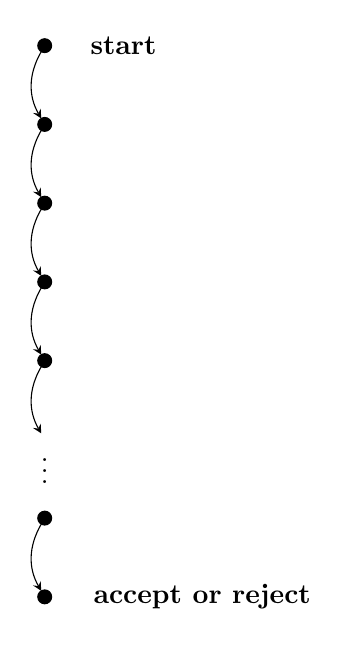
\begin{tikzpicture}[
          auto, >=stealth, node distance=0.0ex and 2em,
          pil/.style={->},
          dot/.style={circle, draw=black, fill=black, minimum size=#1, inner sep=0pt, outer sep=0pt} ]
          %nodes
          \node[dot=5pt, color=black] (start) at (0,10) {};   % start
          \node (s) at (1,10) {\textbf{start}};               % Label start
          \node[dot=5pt, color=black] (v1) at (0,9) {};       % v1
          \node[dot=5pt, color=black] (v2) at (0,8) {};       % v2
          \node[dot=5pt, color=black] (v3) at (0,7) {};       % v3
          \node[dot=5pt, color=black] (v4) at (0,6) {};       % v4
          \node[dot=5pt, color=white] (v5) at (0,5) {};       % v5
          \node (vdots) at (0,4.7) {$\vdots$};
          \node[dot=5pt, color=black] (v6) at (0,4) {};       % v6
          \node[dot=5pt, color=black] (v7) at (0,3) {};       % v7
          \node (a) at (2,3) {\textbf{accept or reject}};  % Label start
          %edges
          \path[pil] (start) edge[bend right] (v1);
          \path[pil] (v1) edge[bend right] (v2);
          \path[pil] (v2) edge[bend right] (v3);
          \path[pil] (v3) edge[bend right] (v4);
          \path[pil] (v4) edge[bend right] (v5);
          \path[pil] (v6) edge[bend right] (v7);
      \end{tikzpicture}
      \caption{Deterministic computation.}
      \label{fig:deterministic}
  \end{subfigure}
  \hspace{5em} % vertical space
  \begin{subfigure}[b]{0.4\textwidth}
    \centering
      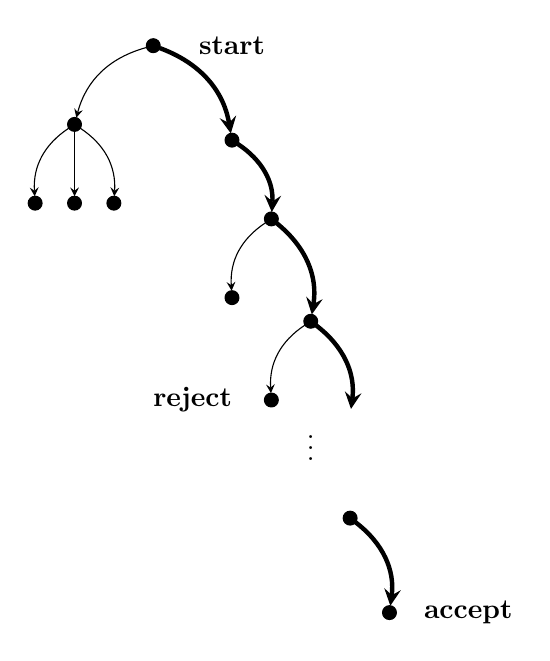
\begin{tikzpicture}[
          auto, >=stealth, node distance=0.0ex and 2em,
          pil/.style={->},
          dot/.style={circle, draw=black, fill=black, minimum size=#1, inner sep=0pt, outer sep=0pt} ]
        %nodes
        \node[dot=5pt, color=black] (start) at (0,10) {};       % start
        \node (s) at (1,10) {\textbf{start}};                   % Label start
        \node[dot=5pt, color=black] (v1) at (-1,9) {};          % v1
        \node[dot=5pt, color=black] (v2) at (1,8.8) {};         % v2
        \node[dot=5pt, color=black] (v3) at (-1.5,8) {};        % v3
        \node[dot=5pt, color=black] (v4) at (-1,8) {};          % v4
        \node[dot=5pt, color=black] (v5) at (-0.5,8) {};        % v5
        \node[dot=5pt, color=black] (v6) at (1.5,7.8) {};       % v6
        \node[dot=5pt, color=black] (v7) at (1,6.8) {};         % v7
        \node[dot=5pt, color=black] (v8) at (2,6.5) {};         % v8
        \node[dot=5pt, color=black] (v9) at (1.5,5.5) {};       % v9
        \node[dot=5pt, color=white] (v10) at (2.5,5.3) {};      % v10
        \node (vdots) at (2,5) {$\vdots$};
        \node[dot=5pt, color=black] (v11) at (2.5,4) {};        % v11
        \node[dot=5pt, color=black] (v12) at (3,2.8) {};        % v12
        \node (a) at (0.5,5.5) {\textbf{reject}};            % Label reject
        \node (b) at (4,2.8) {\textbf{accept}};              % Label accept
        %edges
        \path[pil] (start) edge[bend right] (v1);
        \path[pil, ultra thick] (start) edge[bend left] (v2);
        \path[pil] (v1) edge[bend right] (v3);
        \path[pil] (v1) edge (v4);
        \path[pil] (v1) edge[bend left] (v5);
        \path[pil, ultra thick] (v2) edge[bend left] (v6);
        \path[pil] (v6) edge[bend right] (v7);
        \path[pil, ultra thick] (v6) edge[bend left] (v8);
        \path[pil] (v8) edge[bend right] (v9);
        \path[pil, ultra thick] (v8) edge[bend left] (v10);
        \path[pil, ultra thick] (v11) edge[bend left] (v12);
      \end{tikzpicture}
      \caption{Nondeterministic computation.}
      \label{fig:nondeterministic}
  \end{subfigure}
  \caption{Deterministic and Nondeterministic computations with an accepting branch.}
  \label{fig:computations}
\end{figure}
%%%%%%%%%%%%%%%%%%%%%%%%%%%%%%%%%%%%%%%%%%%%%%%% ENDING OF A FIGURE %%%%%%%%%%%%%%%%%%%%%%%%%%%%%%%%%%%%%%%%%%%%%%%

\subsection{Computational Complexity Classes}\label{subsec:computational-complexity-classes}
Computational complexity theory contemplates not solely the solvability of a problem but also the resources required to solve computational problems.
It is divided in two branches: \textit{Time} complexity and \textit{Space} complexity as mentioned earlier. In this work, we give an informal
description of the classical complexity classes generally encountered. The interested reader can find full details and formal definitions in the
excellent textbook of Sipser \cite{sipserIntroductionTheoryComputation2006}. The following section describes the different computational complexity
classes in which different decision problems fits.

In general, these complexity classes study how the critical ressources (\textit{time} and \textit{space}) grows in terms if the input size.
For decision problems, the input is the description of the problem and its size measured as bits of information.

\subsubsection{Time complexity classes}
We start by characterizing in terms of time. The class $\P$ consists of all problems solvable in polynomial time, that is, all problems solved by
some algorithm in time that is at most linear, quadratic, cubic, or similar in the input size. If $n$ represents the input size, a general polynomial
might look like $5n^{4} + 3n^{2} + 10n - 1$.
Similarly, the class $\EXP$ consists of all problems solvable in exponential time:
$2^{n}, 5^{n}, 2^{n^{2}}$ or in general $2^{p(n)}$ where $p(n)$ is some polynomial. Note that $\EXP$ contains easier problems too, in particular,
all of $\P$.

\subsubsection{Space complexity classes}
On the other hand, the class $\PSPACE$ consists of all problems solvable in polynomial space. This class is the analog of $\P$ but measuring space
instead of time. Similarly, $\EXPSPACE$ consists of all problems solvable in exponential space.

Time and space complexity classes are related in the following way: An optimal algorithm never uses more space than time.
Thus, every problem in $\P$ is also in $\PSPACE$. Also, any (deterministic) algorithm that uses $s$ space can never use more than
exponential-in-$s$ time without repeating a position. Thus, every problem in $\PSPACE$ is also in $\EXP$.

\subsubsection{Nondeterminism}
Next, we consider allowing nondeterminism in order to solve a problem. A nondeterministic algorithm can at any computation step, proceed with
various possibilities (see Fig.~\ref{fig:nondeterministic}). A nondeterministic algorithm can be thought of as an extremly lucky: whenever it needs
to make a decision, it by defintion makes the correct choice. The class $\NP$ consists of all problems that can be solved in polynomial time by such a
nondeterministic algorithm. Similarly, we can define $\NPSPACE$ for the nondeterministic analog of $\PSPACE$, and $\NEXP$ for $\EXP$.

\subsubsection{Completeness}
For each complexity class $X$, we call a problem $X$-hard if it is about as hard as every problem in $X$. (Here, we ignore polynomial factors in the
difficulty.) We call a problem $X$-complete if it is both $X$-hard and in $X$. Thus, for example, $\NP$-complete problems are among the hardest problems
in $\NP$, so they must not be in any strictly easier complexity class. Whether $\P = \NP$ is of course a major open problem, but assuming they are even
slightly different, $\NP$-complete problems are not in $\P$. Thus, when classifying a problem into a particular complexity class, showing that the problem
is amongst the hardest problems in a certain complexity class eliminates any doubt of whether the latter belongs in a lower complexity class.
One technique of doing so is by \textit{reduction}.

\paragraph{Reducibility}
By taking a known $X$-complete problem $(B)$ and showing that solving the problem in which we are interested $(A)$ is at least as hard as solving $B$,
we can conclude that $A$ is $X$-hard. We usually do this by showing a way to transform problem $B$ into problem $A$.
\begin{defn}
A function $f : \Sigma^{*} \rightarrow \Sigma^{*}$ is a computable function if on every input $w$, some Turing machine $M$ halts with just $f(w)$ on its tape.
\end{defn}

\begin{defn}
Given two languages $A$ and $B$, $B$ is reducible to $A$ written $B \leq_{p} A$ if there is a computable function $f : \Sigma^{*} \rightarrow \Sigma^{*}$, where for
every $w, w \in B \Longleftrightarrow f(w) \in B$. The function $f$ is called the reduction of $B$ to $A$.
\end{defn}

\subsubsection{Relationship of Complexity Classes} \cite{hearn_demaine_ncl_book}
So far we have that $\P \subseteq \PSPACE \subseteq \EXP$. $\PSPACE = \NPSPACE$ follows from the celebrated result of Savitch \cite{savitch_relationships_1970}.
Concerning nondeterminism, a nondeterministic computation is at least as powerful as regular deterministic computation, so, for example, every problem
in $\P$ is also in $\NP$. On the other hand, nondeterministic computation can be simulated by trying both choices of each decision in turn, which
takes exponentially more time, but about the same amount of space. Thus, for example, every problem in $\NP$ is also in $\PSPACE$. Summing all
together, we can conclude that :
\begin{center}
  $\P \subseteq \NP \subseteq \PSPACE = \NPSPACE \subseteq \EXP \subseteq \NEXP \subseteq \EXPSPACE$
\end{center}
All of the containments are believed to be strict, but beyond the above relations, the only strict containment known among those
classes is $\P  \subsetneq \EXP$. Whether $\P = NP$ is the most famous unresolved question in Computational Complexity Theory.


\section{Reconfiguration Graph}
Viewing Reconfiguration problems from a graph-theoretic perspective, the notion of a \textit{reconfiguration graph} naturally arises.
Let $G = (V, E)$ be a reconfiguration graph where $V(G)$ is the vertex set consisting of all possible configurations and two nodes are
connected by an edge if the corresponding configurations can each be obtained from the other by the application of a single transformation rule,
\textit{a reconfiguration step}. Any path or walk in the reconfiguration graph corresponds to a sequence of reconfiguration steps called a
\textit{reconfiguration sequence}. Although the terminology concerning reconfiguration problems has not yet stabilized in the litterature those are
the terms that will be used throughout this work.

\chapter{The Nondeterministic Constraint Logic (NCL)} \label{chap:NCL}
In this chapter, the Nondeterministic Constraint Logic model of computation is presented. This framework developed by Demaine and Hearn is
motivated by the Sliding-block puzzles \cite{hordern_sliding_1986}. The main result of \cite{hearn_pspace-completeness_2004} introduces the new
nondeterministic model of computation based on reversing edge directions in weighted directed graphs with minimum in-flow constraints on vertices.
This model, referred to as Nondeterministic Constraint Logic, or NCL, is shown to have the same computational power as a space-bounded Turing machine.

Several decision problems in the NCL framework are proved to be $\PSPACE$-complete \cite{hearn_pspace-completeness_2004}. These decision problems are then used to prove the
$\PSPACE$-completeness of well-known Sliding-block puzzles such as Rush Hour and Sokoban \cite{hearn_demaine_ncl_book}. Demaine and Hearn argue that NCL can be considered as a
model of computation in its own right instead of just a set of decision problems. Thus, proving a problem to be $\PSPACE$-hard in the NCL
framework simply requires the construction of a couple of gadgets that can be connected together.
In the last section of \cite{hearn_pspace-completeness_2004} gives an interesting equivalent formulation of NCL in terms of sliding tokens along
graph edges. This latter formulation will be the focus of sections \ref{sec:sliding_tokens} and \ref{sec:labelled_sliding_token} to prove that
the Sliding token problem and labelled variant of the sliding token problem are $\PSPACE$-complete (theorems \ref{theorem:ncl_sliding_token}
and \ref{theorem:labelled} respectively).

\textit{Roadmap.} Section \ref{sec:formalism} describes the constraint logic using a graph formulation.
Section \ref{sec:contraint_graph} gives an overview of AND/OR constraint graphs which is the primary formulation used in the NCL framework.
Section \ref{sec:ncl_results} present some complexity results of decision problems stemming from the constraint logic framework.
In section \ref{sec:sliding_tokens} we detail the $\PSPACE$-completeness proof of the sliding token problem using the alternative
formulation of NCL (theorem \ref{theorem:ncl_sliding_token}). Lastly, in section \ref{sec:labelled_sliding_token} the hardness proof of the
labelled variant of the sliding token problem is given.

\section{Graph Formulation}\label{sec:formalism}
The simplest description of NCL is a graph formulation. An NCL machine consists of a \textit{constraint graph}, $G = (V,E)$ that we can think of as
our computation model. Let $G$ be an undirected graph to which each edge is assigned a nonnegative integer and each vertex has a
nonnegative \textit{minimum inflow constraint}. A \textit{configuration} of this machine is an orientation (direction) of the edges such that the sum
of incoming edge weights at each vertex is at least the minimum in-flow constraint of that vertex. A \textit{move} from one
configuration to another configuration is simply the reversal of a single edge such that the minimum in-flow constraints remain satisfied.


\section{AND/OR Constraint Graphs} \label{sec:contraint_graph}
As part of the constraint logic framework,  Hearn and Demaine provided a restricted variant of Nondeterministic Constraint Logic (restricted NCL),
in which the constraint graph $G$ is planar, $3$-regular, uses only weights $ \in \{1,2\}$ (referred to as red and blue edges respectively), the minimum
in-flow = $2$ and the graph is constructed from only two specific vertex types ($AND$ and $OR$ vertices). A vertex $v$ of $G$ is an \textit{AND vertex}
if exactly one incident edge has weight $2$ (Figure \ref{fig:and_vertex}) and a vertex $v$ of $G$ is an \textit{OR vertex} if all the incident edges
have weight $2$ (Figure \ref{fig:or_vertex}). Thus, a graph $G$ is an \textit{AND/OR constraint graph} if it consists of only $AND$ and $OR$ vertices.

%%%%%%%%%%%%%%%%%%%%%%%%%%%%%% BEGINING OF A FIGURE : AND and OR vertex of constraint graph %%%%%%%%%%%%%%%%%%%%%%%%%%%%%
\begin{figure}[H]
  \begin{subfigure}[b]{0.4\textwidth}
    \centering
      \begin{scaletikzpicturetowidth}{\textwidth}
        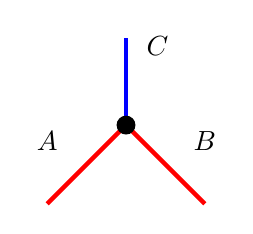
\begin{tikzpicture}
          \def\xa{0}     % AND
          \def\ya{0}
          %labels
          \node (1) at (\xa+0.4,\ya+1) {$C$};
          \node (2) at (\xa+1,\ya-0.2) {$B$};
          \node (2) at (\xa-1,\ya-0.2) {$A$};
          % f_1 arrows
          \draw[ultra thick, -, blue] (\xa, \ya) -- (\xa, \ya+1.1);
          \draw[ultra thick, -, red] (\xa, \ya) -- (\xa+1, \ya-1);
          \draw[ultra thick, -, red] (\xa, \ya) -- (\xa-1, \ya-1);
          % Nodes fill
          \path[fill] (\xa,\ya) circle (\ver);
        \end{tikzpicture}
      \end{scaletikzpicturetowidth}
      \caption{And vertex. Edge $C$ may be directed outward if and only if edges $A$ and $B$ are both directed inward.}
      \label{fig:and_vertex}
  \end{subfigure}
  \hspace{5em} % vertical space
  \begin{subfigure}[b]{0.4\textwidth}
    \centering
    \begin{scaletikzpicturetowidth}{\textwidth}
      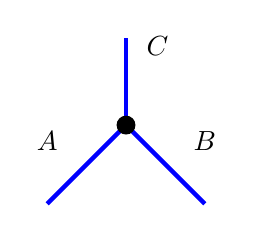
\begin{tikzpicture}
        \def\xb{5} % OR
        \def\yb{0}
        %labels
        \node (1) at (\xb+0.4,\yb+1) {$C$};
        \node (2) at (\xb+1,\yb-0.2) {$B$};
        \node (2) at (\xb-1,\yb-0.2) {$A$};
        % f_2 arrows
        \draw[ultra thick, -, blue] (\xb, \yb) --(\xb, \yb+1.1);
        \draw[ultra thick, -, blue] (\xb, \yb) --(\xb+1, \yb-1);
        \draw[ultra thick, -, blue] (\xb, \yb) --(\xb-1, \yb-1);
        % Nodes fill
        \path[fill] (\xb,\yb) circle (\ver);     % OR
      \end{tikzpicture}
    \end{scaletikzpicturetowidth}
    \caption{Or vertex. Edge $C$ may be directed outward if and only if either edge $A$ or edge $B$ is directed inward.}
    \label{fig:or_vertex}
  \end{subfigure}
  \caption{And and Or vertices. Red edges have weight $1$, blue edges have weight $2$, and all vertices have a minimum in-flow constraint of $2$.}
  \label{fig:and_or_vertices}
\end{figure}
%%%%%%%%%%%%%%%%%%%%%%%%%%%%%%%%%%%%%%%% ENDING OF A FIGURE %%%%%%%%%%%%%%%%%%%%%%%%%%%%%%%%%

\section{NCL Results} \label{sec:ncl_results}
This section compiles the important complexity results linked to NCL. A first fundamental decision problem that arises in the NCL framework
is about the satisfiability of a given constraint graph $G$. It is defined as follows :
\begin{flushleft}
  CONSTRAINT GRAPH SATISFIABILITY \\
  \textbf{Instance: } A constraint graph $G$. \\
  \textbf{Question: } Does $G$ have a legal configuration ? \\
\end{flushleft}
In \cite{hearn_demaine_ncl_book} Demaine and Hearn proved that the CONSTRAINT GRAPH SATISFIABILITY problem is $\NP-$complete.

Another important problem regarding constraint graphs is about their reconfigurability. The CONFIGURATION-TO-CONFIGURATION (C2C) problem asks
if given two configurations of a constraint graph $G$, whether they can be reconfigured into each other.
\begin{flushleft}
  CONFIGURATION-TO-CONFIGURATION (C2C)\\
  \textbf{Instance: } A constraint graph $G$ and two legal configurations $C_1, C_2$ for $G$. \\
  \textbf{Question: } Is there a sequence of legal configurations from $C_0, C_1, \dots , C_t$ such that $C_i$ is obtained from $C_{i-1}$
  by a legal move for each $i$ with $1 \leq i \leq t$ and $C_0 = C_1, C_t = C_2$ ? \\
\end{flushleft}
Hearn and Demaine established that the C2C problem is $\PSPACE$-complete\cite{hearn_demaine_ncl_book}.

Similar to the C2C problem, the CONFIGURATION-TO-EDGE (C2E) problem asks whether a target edge $e$ can be reversed
given a constraint graph $G$.
\begin{flushleft}
  CONFIGURATION-TO-EDGE (C2E) \\
  \textbf{Instance: } A constraint graph $G$, a target edge $e$ from $G$ and an initial legal configuration $C$ for $G$ . \\
  \textbf{Question: } Is there a sequence of legal configurations, starting with $C$, where every configuration is obtained from the previous
  by changing the orientation of one edge, so that $e$ is eventually reversed? \\
\end{flushleft}
Hearn and Demaine proved that the C2E problem is also $\PSPACE$-complete\cite{hearn_demaine_ncl_book}.

More interestingly, the hardness result for C2C and C2E still holds when the vertices of $G$ are restricted to be $AND$ and $OR$ vertices
defined in section \ref{sec:contraint_graph} ans referred as restricted NCL. C2C and C2E hardness proof involves a reduction from quantified
Boolean formulas, based on the logical interpretation of AND/OR constraint graphs. Additional gadgets are required for simulating quantifiers
and for converting red edges into blue edges (and vice versa), which can all be accomplished by combinations of $AND$ and $OR$
vertices \cite{hearn_demaine_ncl_book}.

Demaine and Hearn in fact strengthen this result even further and show that C2C and C2E both remain $\PSPACE$-complete when the constraint
graph $G$ is planar \cite{hearn_demaine_ncl_book}. This proof involves the construction of crossover gadgets that allow two edges to cross
each other.

It is also possible to impose an additional restriction, while preserving the hardness of these problems: each vertex with three blue edges
can be required to be part of a triangle with a red edge. Such a vertex is called a protected or, and it has the property that
(in any valid orientation of the whole graph) it is not possible for both of the blue edges in the triangle to be directed inwards.
This restriction makes it easier to simulate these vertices in hardness reductions for other problems\cite{hearn_demaine_ncl_book}.
Additionally, the constraint graphs can be required to have bounded bandwidth, and the problems on them will still remain
$\PSPACE$-complete\cite{van_der_zanden_parameterized_nodate}.


\section{Alternative formulation : Sliding tokens} \label{sec:sliding_tokens}
The SLIDING TOKEN problem was introduced by Hearn and Demaine in \cite{hearn_pspace-completeness_2004} as a variant of SLIDING-BLOCK puzzle
with $1 \times 1 $ blocks on a graph but require no adjacent tokens, which can be seen as a reconfiguration problem for Independent Set.
Suppose that we are given two independent sets $I_b$ and $I_r$ of a graph $G =(V,E)$ such that $|I_b| = |I_r|$ and imagine that a
\textit{token} is placed on each vertex in $I_b$. Then, the SLIDING TOKEN problem is to determine whether there exists a sequence
$ S = \langle I_1, I_2, \dots, I_l \rangle$ of independent sets of $G$ such that :
\begin{enumerate}
  \item $I_1 = I_b, I_l = I_r,$ and $|I_i| = |I_b| = |I_r|$ for all $i, 1 \leq i \leq l;$ and
  \item For each $i, 2 \leq i \leq l$ there is an edge $xy$ in $G$ such that  $I_{i-1} \setminus I_{i} = \{x\}$ and $I_{i} \setminus I_{i-1} = \{y\}$.
\end{enumerate}
That is, $I_i$ can be obtained from $I_{i-1}$ by sliding exactly one token on a vertex $x \in I_{i-1}$ to its adjacent vertex $y \in I_{i}$
along an edge $xy \in E(G)$. Such a sequence $S$, if exists, is called a \textit{TS-sequence} in $G$ between $I_b$ and $I_r$.
We denote by a $3$-tuple $(G, I_{b}, I_{r})$ an instance of SLIDING TOKEN problem.  If a TS-sequence $S$ in $G$ between $I_{b}$ and $I_{r}$ exists,
we say that $I_{b}$ is \textit{reconfigurable} to $I_{r}$ (and vice versa), and write $I_{b} \overset{G}\leftrightsquigarrow I_{r}$. The sets
$I_{b}$ and $I_{r}$ are the \textit{initial} and \textit{target} independent sets, respectively. For a TS-sequence $S$, the \textit{length}
len($S$)of $S$ is defined as the number of independent sets in $S$ minus one. In other words, len($S$) is the number of \textit{token-slides}
described in $S$. Figure \ref{fig:sliding_token_example} illustrates a TS-sequence of length $4$ between two independent sets
$I_{b} = I_{1}$ and $I_{r} = I_{5}$.

\begin{figure}[H]
  \centering
    \begin{scaletikzpicturetowidth}{\textwidth}
      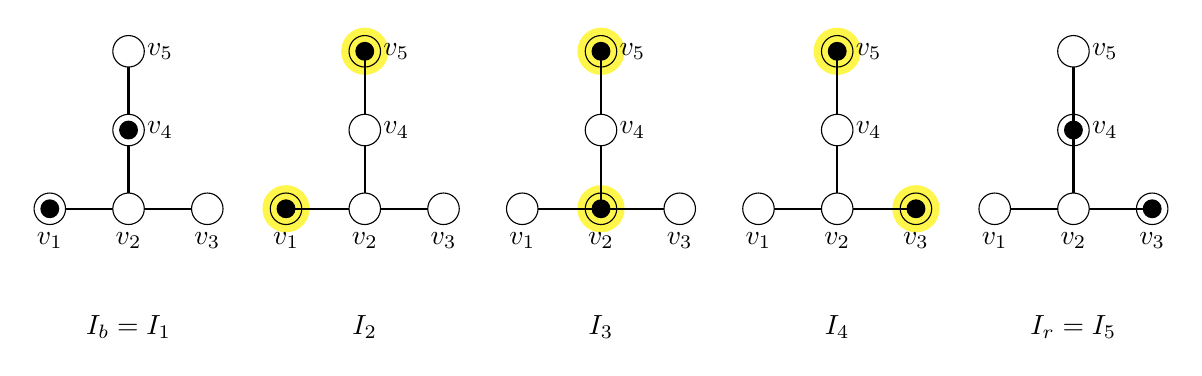
\begin{tikzpicture}[scale=1]
        \def\x{1}
        \def\xa{0}
        \def\ya{0}
        \def\xb{3}
        \def\xc{6}
        \def\xd{9}
        \def\xe{12}

        %graph G
        %edges
        \draw[thick] (\xa,\ya)--(\xa+1,\ya)--(\xa+1,\ya+1)--(\xa+1,\ya+2);
        \draw[thick] (\xa+1,\ya)--(\xa+2,\ya);
        %nodes
        \draw[fill=white] (\xa,\ya) circle (0.2cm);     %v1
        \draw[fill=white] (\xa+1,\ya+1) circle (0.2cm); %v2
        \draw[fill=white] (\xa+1,\ya+2) circle (0.2cm); %v3
        \draw[fill=white] (\xa+2,\ya) circle (0.2cm);   %v4
        \draw[fill=white] (\xa+1,\ya) circle (0.2cm);   %v5
        % Tokens
        \path[fill] (\xa+1,\ya+1) circle (\ver);
        \path[fill] (\xa,\ya) circle (\ver);
        %labels
        \node (1) at (\xa,\ya-0.4) {$v_1$};
        \node (2) at (\xa+1+0.4,\ya+1) {$v_4$};
        \node (3) at (\xa+1+0.4,\ya+2) {$v_5$};
        \node (5) at (\xa+2,\ya-0.4) {$v_3$};
        \node (4) at (\xa+1,\ya-0.4) {$v_2$};
        \node (1) at (\xa+1,\ya-1.5) {$I_b = I_1$};

        %G_1
        % Highlights
        \draw[fill=yellow, opacity=.7, draw=none] (\xb+1,\ya+2) circle (0.3cm);
        \draw[fill=yellow, opacity=.7, draw=none] (\xb,\ya)  circle (0.3cm);
        %edges
        \draw[thick] (\xb,\ya)--(\xb+1,\ya)--(\xb+1,\ya+1)--(\xb+1,\ya+2);
        \draw[thick] (\xb+1,\ya)--(\xb+2,\ya);
        %nodes
        \draw             (\xb,\ya) circle (0.2cm);    %v1
        \draw[fill=white] (\xb+1,\ya+1) circle (0.2cm);%v2
        \draw             (\xb+1,\ya+2) circle (0.2cm);%v3
        \draw[fill=white] (\xb+2,\ya) circle (0.2cm);  %v4
        \draw[fill=white] (\xb+1,\ya) circle (0.2cm);  %v5
        % Tokens
        \path[fill] (\xb+1,\ya+2) circle (\ver);
        \path[fill] (\xb,\ya) circle (\ver);
        %labels
        \node (1) at (\xb,\ya-0.4) {$v_1$};
        \node (2) at (\xb+1+0.4,\ya+1) {$v_4$};
        \node (3) at (\xb+1+0.4,\ya+2) {$v_5$};
        \node (5) at (\xb+2,\ya-0.4) {$v_3$};
        \node (4) at (\xb+1,\ya-0.4) {$v_2$};
        \node (1) at (\xb+1,\ya-1.5) {$I_2$};

        %G_2
        % Highlights
        \draw[fill=yellow, opacity=.7, draw=none] (\xc+1,\ya+2) circle (0.3cm);
        \draw[fill=yellow, opacity=.7, draw=none] (\xc+1,\ya)  circle (0.3cm);
        %edges
        \draw[thick] (\xc,\ya)--(\xc+1,\ya)--(\xc+1,\ya+1)--(\xc+1,\ya+2);
        \draw[thick] (\xc+1,\ya)--(\xc+2,\ya);
        %nodes
        \draw[fill=white] (\xc,\ya) circle (0.2cm);    %v1
        \draw[fill=white] (\xc+1,\ya+1) circle (0.2cm);%v2
        \draw             (\xc+1,\ya+2) circle (0.2cm);%v3
        \draw[fill=white] (\xc+2,\ya) circle (0.2cm);  %v4
        \draw             (\xc+1,\ya) circle (0.2cm);  %v5
        % Tokens
        \path[fill] (\xc+1,\ya+2) circle (\ver);
        \path[fill] (\xc+1,\ya)  circle (\ver);
        %labels
        \node (1) at (\xc,\ya-0.4) {$v_1$};
        \node (2) at (\xc+1+0.4,\ya+1) {$v_4$};
        \node (3) at (\xc+1+0.4,\ya+2) {$v_5$};
        \node (5) at (\xc+2,\ya-0.4) {$v_3$};
        \node (4) at (\xc+1,\ya-0.4) {$v_2$};
        \node (1) at (\xc+1,\ya-1.5) {$I_3$};

        %G_3
        % Highlights
        \draw[fill=yellow, opacity=.7, draw=none] (\xd+1,\ya+2) circle (0.3cm);
        \draw[fill=yellow, opacity=.7, draw=none] (\xd+2,\ya)  circle (0.3cm);
        %edges
        \draw[thick] (\xd,\ya)--(\xd+1,\ya)--(\xd+1,\ya+1)--(\xd+1,\ya+2);
        \draw[thick] (\xd+1,\ya)--(\xd+2,\ya);
        %nodes
        \draw[fill=white] (\xd,\ya) circle (0.2cm);    %v1
        \draw[fill=white] (\xd+1,\ya+1) circle (0.2cm);%v2
        \draw             (\xd+1,\ya+2) circle (0.2cm);%v3
        \draw             (\xd+2,\ya) circle (0.2cm);  %v4
        \draw[fill=white] (\xd+1,\ya) circle (0.2cm);  %v5
        % Tokens
        \path[fill] (\xd+1,\ya+2)  circle (\ver);
        \path[fill] (\xd+2,\ya) circle (\ver);
        %labels
        \node (1) at (\xd,\ya-0.4) {$v_1$};
        \node (2) at (\xd+1+0.4,\ya+1) {$v_4$};
        \node (3) at (\xd+1+0.4,\ya+2) {$v_5$};
        \node (5) at (\xd+2,\ya-0.4) {$v_3$};
        \node (4) at (\xd+1,\ya-0.4) {$v_2$};
        \node (1) at (\xd+1,\ya-1.5) {$I_4$};

        %G4
        %edges
        \draw[thick] (\xe,\ya)--(\xe+1,\ya)--(\xe+1,\ya+1)--(\xe+1,\ya+2);
        \draw[thick] (\xe+1,\ya)--(\xe+2,\ya);
        %nodes
        \draw[fill=white] (\xe,\ya) circle (0.2cm);    %v1
        \draw             (\xe+1,\ya+1) circle (0.2cm);%v2
        \draw[fill=white] (\xe+1,\ya+2) circle (0.2cm);%v3
        \draw             (\xe+2,\ya) circle (0.2cm);  %v4
        \draw[fill=white] (\xe+1,\ya) circle (0.2cm);  %v5
        % Tokens
        \path[fill] (\xe+1,\ya+1)  circle (\ver);
        \path[fill] (\xe+2,\ya) circle (\ver);
        %labels
        \node (1) at (\xe,\ya-0.4) {$v_1$};
        \node (2) at (\xe+1+0.4,\ya+1) {$v_4$};
        \node (3) at (\xe+1+0.4,\ya+2) {$v_5$};
        \node (5) at (\xe+2,\ya-0.4) {$v_3$};
        \node (4) at (\xe+1,\ya-0.4) {$v_2$};
        \node (1) at (\xe+1,\ya-1.5) {$I_r = I_5$};
      \end{tikzpicture}
    \end{scaletikzpicturetowidth}
  \caption{TS sequence $ \langle I_1, I_2,\dots,I_5 \rangle$ of independent sets which transforms $I_b = I_1$ into $I_r = I_5$ where the vertices in independent sets are depicted by small black circles (tokens).}
  \label{fig:sliding_token_example}
\end{figure}

\subsection{Known results for the SLIDING TOKEN problem.}
Analogous to the Independent Set problem being the key problem among thousands of $\NP$-complete problems to prove $\NP$-hardness,
the SLIDING TOKEN problem plays an important role since several $\PSPACE$-hardness results have been proved using reductions from it.

For the sliding token problem, some polynomial time algorithms have been investigated as follows: Linear time algorithms have been shown
for cographs (also known as P4-free graphs) \cite{kaminski_complexity_2012} and trees \cite{2014arXiv1406.6576D}. Polynomial time algorithms
are shown for bipartite permutation graphs \cite{fox-epstein_sliding_2015}, and claw-free graphs \cite{bonsma_reconfiguring_2014}.
On the other hand, $\PSPACE$-completeness is shown for graphs of bounded treewidth \cite{mouawad_reconfiguration_2014}, and planar
graphs \cite{hearn_pspace-completeness_2004}.

\subsection{$\PSPACE$-completeness.}

In this section we go over the $\PSPACE$-completeness result of the SLIDING TOKEN problem, proved by a reduction from NCL. As seen in
section \ref{sec:ncl_results}, there are slightly different versions of decision problems for NCL and all of them are $\PSPACE-$complete.
For our purpose, we just need the version for the configuration-to-configuration for planar NCL. Recall that an instance of the
C2C planar NCL problem is defined on a $3-$regular, planar, directed graph where each edge has a weight $\in \{1,2\}$ and each vertex is
either and $AND$ or an $OR$ vertex. The proof of theorem \ref{theorem:ncl_sliding_token} is organised in sections
\ref{subsubsection:reduction_structure} to \ref{subsubsection:and_or} which explains the reduction structure, gadgets used and how they are
connected together.

\subsubsection{Reduction structure.}\label{subsubsection:reduction_structure}
To show that the SLIDING TOKEN problem is $\PSPACE$-complete we provide a reduction from configuration-to-configuration for AND/OR graphs
such that the NCL instance is solvable if and only if the corresponding SLIDING TOKEN is solvable. The sliding token instance is constructed by
piecing together gadgets which emulates the directed edges, the AND vertices and the OR vertices of the given NCL instance.
We construct the corresponding NCL $AND$ and $OR$ vertex gadgets out of sliding-token subgraphs illustrated in figures
\ref{fig:and_gadget_sliding_token} and \ref{fig:or_gadget_sliding_token} respectively.

\subsubsection{The OR gadget and the AND gadget.}\label{subsubsection:or_and}
The construction of Fig.\ref{fig:and_gadget_sliding_token} satisfies the same constraints as an NCL $AND$ vertex, with the upper
token corresponding to the blue edge and both lower tokens corresponding to the red edges. The upper token can slide in only when both lower
tokens are slid out thus maintaining the flow constraint of an NCL AND vertex.
Likewise, the construction of Fig.\ref{fig:or_gadget_sliding_token} satisfies the same constraints as an NCL $OR$ vertex with the upper
and two lower tokens corresponding the the $OR$ blue edges. The upper token in the $OR$ gadget can slide in when  either lower token is slid
out and the internal token can then slide to one side or the other to make room. Here it is the internal token that ensures the NCL flow
constraint is satisfied by sliding on a appropriate vertex among the three internal nodes to force one among the outer tokens are slid in.

%%%%%%%%%%%%%%%%%%%%%%%%%%%%%%%%%%%%%%%%%%%% BEGINING OF A FIGURE : AND and OR gadget of Sliding Token %%%%%%%%%%%%%%%%%%%%%%%%%%%%%%%%%%%%
\begin{figure} [H]
  \begin{subfigure}[b]{0.4\textwidth}
    \centering
    \begin{scaletikzpicturetowidth}{\textwidth}
      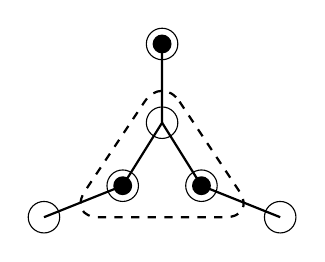
\begin{tikzpicture}
        \def\xa{0}
        \def\ya{0}
        %graph G
        \draw (\xa,\ya) circle (0.2cm);          %v1 no fill
        \draw (\xa,\ya+1) circle (0.2cm);        %v2 no fill
        \draw (\xa+0.5,\ya-0.8) circle (0.2cm);  %v4 no fill
        \draw (\xa-0.5,\ya-0.8) circle (0.2cm);  %v3 no fill
        \draw (\xa-1.5,\ya-1.2) circle (0.2cm);  %v5 no fill
        \draw (\xa+1.5,\ya-1.2) circle (0.2cm);  %v6 no fill
        \path[fill] (\xa,\ya+1) circle (\ver);       %v2
        \path[fill] (\xa+0.5,\ya-0.8) circle (\ver); %v4
        \path[fill] (\xa-0.5,\ya-0.8) circle (\ver); %v3
        %labels
        \draw[thick] (\xa,\ya+1)--(\xa,\ya)--(\xa-0.5,\ya-0.8)--(\xa-1.5,\ya-1.2);
        \draw[thick] (\xa,\ya)--(\xa+0.5,\ya-0.8)--(\xa+1.5,\ya-1.2);
        \path[draw, thick, dashed, rounded corners=4mm] (\xa,\ya+0.6)--(\xa+1.2,\ya-1.2)--(\xa-1.2,\ya-1.2)--cycle;
      \end{tikzpicture}
    \end{scaletikzpicturetowidth}
    \caption{$AND$ gadget}
    \label{fig:and_gadget_sliding_token}
  \end{subfigure}
  \hspace{3em} % vertical space
  \begin{subfigure}[b]{0.4\textwidth}
    \centering
    \begin{scaletikzpicturetowidth}{\textwidth}
      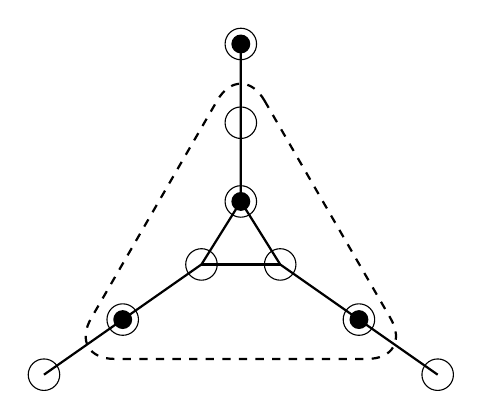
\begin{tikzpicture}
        \def\xb{5}
        \def\yb{0}
        %G_1
        \draw (\xb,\yb+2) circle (0.2cm);         %v9
        \draw (\xb,\yb) circle (0.2cm);           %v1
        \draw (\xb+0.5,\yb-0.8) circle (0.2cm);   %v4
        \draw (\xb-0.5,\yb-0.8) circle (0.2cm);   %v3
        \draw (\xb,\yb+1) circle (0.2cm);         %v2
        \draw (\xb-1.5,\yb-1.5) circle (0.2cm);   %v5
        \draw (\xb+1.5,\yb-1.5) circle (0.2cm);   %v6
        \draw (\xb-2.5,\yb-2.2) circle (0.2cm);     %v7
        \draw (\xb+2.5,\yb-2.2) circle (0.2cm);     %v8

        \path[fill] (\xb,\yb+2) circle (\ver);         %v0
        \path[fill] (\xb,\yb) circle (\ver);           %v1
        \path[fill] (\xb-1.5,\yb-1.5) circle (\ver);   %v5
        \path[fill] (\xb+1.5,\yb-1.5) circle (\ver);   %v6
        %labels
        \draw[thick] (\xb,\yb+2)--(\xb,\yb+1)--(\xb,\yb)--(\xb-0.5,\yb-0.8)--(\xb-1.5,\yb-1.5)--(\xb-2.5,\yb-2.2);
        \draw[thick] (\xb,\yb)--(\xb+0.5,\yb-0.8)--(\xb+1.5,\yb-1.5)--(\xb+2.5,\yb-2.2);
        \draw[thick] (\xb-0.5,\yb-0.8)--(\xb+0.5,\yb-0.8);
        \path[draw, thick, dashed, rounded corners=6mm] (\xb,\yb+1.8)--(\xb+2.2,\yb-2)--(\xb-2.2,\yb-2)--cycle;
      \end{tikzpicture}
    \end{scaletikzpicturetowidth}
    \caption{$OR$ gadget}
    \label{fig:or_gadget_sliding_token}
  \end{subfigure}
  \caption{Sliding Tokens vertex gadgets.}
  \label{fig:and_or_gadgets_sliding_token}
\end{figure}
%%%%%%%%%%%%%%%%%%%%%%%%%%%%%%%%%%%%%%%%%%%%%%%% ENDING OF A FIGURE %%%%%%%%%%%%%%%%%%%%%%%%%%%%%%%%%%%%%%%%%%%%%%%%

\subsubsection{AND/OR Graphs}\label{subsubsection:and_or}
We showed how to construct $AND$ and $OR$ vertices. We now show how to connect the vertices into an arbitrary planar constraint graph.
First, the edges that cross the dotted-line gadget borders are called “port” edges. A token on an outer port-edge vertex represents an
inward-directed NCL edge, and vice-versa. Second, observe that no port token may ever leave its port edge. Choosing a particular port
edge $E$, if we inductively assume that this condition holds for all other port edges, then there is never a legal move outside $E$ for
its token – another port token would have to leave its own edge first.
Given an $AND/OR$ graph $G$ and two legal configurations $C_1, C_2$ for $G$, we construct a corresponding sliding-token graph by joining together
$AND$ and $OR$ vertex gadgets at their shared port edges, placing the port tokens appropriately.


\begin{theorem}Sliding Token problem is $\PSPACE$-complete. \end{theorem}\label{theorem:ncl_sliding_token}
\begin{proof}
  First, we show that SLIDING TOKEN problem is in $\PSPACE$.
  The SLIDING TOKEN problem is in $\PSPACE$ since the state of the input graph can be described in a linear number of bits, specifying the
  position of each token and the list of possible moves from any state can be computed in polynomial time. Thus we can nondeterministically
  traverse the state space, at each step nondeterministically choosing a move to make, and maintaining the current state but not the previously
  visited states showing that SLIDING TOKEN is in $\NPSPACE$. By Savitch's celebrated theorem, we have that $\NPSPACE = \PSPACE$
  \cite{savitch_relationships_1970}, implying that SLIDING TOKEN is in $\PSPACE$.

  The SLIDING TOKEN problem is $\PSPACE$-hard by a reduction from planar Nondeterministic Constraint Logic using the reduction structure
  provided above. The NCL instance is solvable if and only if the corresponding SLIDING TOKEN is solvable.
\end{proof}

\begin{example}{C2E to SLIDING TOKEN problem reduction. \\}
\textbf{Input instance : C2E for restricted NCL.} \hfill

\begin{figure}[H]
  \centering
  \begin{subfigure}[b]{0.4\textwidth}
    \begin{scaletikzpicturetowidth}{\textwidth}
      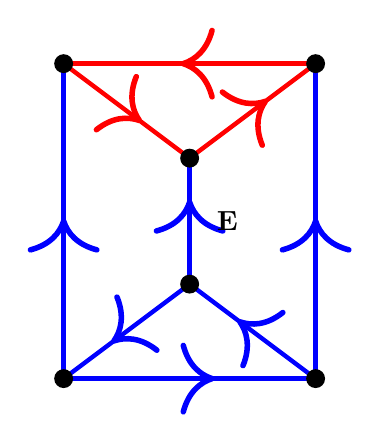
\begin{tikzpicture}[scale=0.8]
        \def\ver{0.15} %size of a vertex
        % v1
        \def\xa{0}
        \def\ya{0}
        % arrows
        \draw[middlearrow={<}, red] (\xa-2,\ya+1.5)-- (\xa+2,\ya+1.5);        % v2 - v3
        \draw[middlearrow={<}, red] (\xa+2,\ya+1.5) -- (\xa,\ya);             % v3 - v1
        \draw[middlearrow={<}, red] (\xa,\ya) -- (\xa-2,\ya+1.5);             % v1 - v2
        \draw[middlearrow={<}, blue] (\xa-2,\ya+1.5) -- (\xa-2,\ya-3.5);      % v2 - v4
        \draw[middlearrow={<}, blue] (\xa,\ya) -- (\xa,\ya-2);                % v1 - v6
        \draw[middlearrow={<}, blue] (\xa+2,\ya+1.5) -- (\xa+2,\ya-3.5);      % v3 - v5
        \draw[middlearrow={>}, blue] (\xa-2,\ya-3.5) -- (\xa+2,\ya-3.5);      % v4 - v5
        \draw[middlearrow={<}, blue] (\xa-2,\ya-3.5) -- (\xa,\ya-2);          % v4 - v6
        \draw[middlearrow={<}, blue] (\xa,\ya-2) -- (\xa+2,\ya-3.5);          % v6 - v5
        % edges
        \draw[ultra thick, -, red] (\xa-2,\ya+1.5) -- (\xa+2,\ya+1.5);       % v2 - v3
        \draw[ultra thick, -, red] (\xa+2,\ya+1.5) -- (\xa,\ya);             % v3 - v1
        \draw[ultra thick, -, red] (\xa,\ya) -- (\xa-2,\ya+1.5);             % v1 - v2
        \draw[ultra thick, -, blue] (\xa-2,\ya+1.5) -- (\xa-2,\ya-3.5);      % v2 - v4
        \draw[ultra thick, -, blue] (\xa,\ya) -- (\xa,\ya-2);                % v1 - v6
        \draw[ultra thick, -, blue] (\xa+2,\ya+1.5) -- (\xa+2,\ya-3.5);      % v3 - v5
        \draw[ultra thick, -, blue] (\xa-2,\ya-3.5) -- (\xa+2,\ya-3.5);      % v4 - v5
        \draw[ultra thick, -, blue] (\xa-2,\ya-3.5) -- (\xa,\ya-2);          % v4 - v6
        \draw[ultra thick, -, blue] (\xa,\ya-2) -- (\xa+2,\ya-3.5);          % v6 - v5

        \node (a) at (\xa+0.6,\ya-1) {\textbf{E}};

        %graph G : Nodes fill
        \path[fill] (\xa,\ya) circle (\ver);           %v1
        \path[fill] (\xa-2,\ya+1.5) circle (\ver);     %v2
        \path[fill] (\xa+2,\ya+1.5) circle (\ver);     %v3
        \path[fill] (\xa-2,\ya-3.5) circle (\ver);     %v4
        \path[fill] (\xa+2,\ya-3.5) circle (\ver);     %v5
        \path[fill] (\xa,\ya-2) circle (\ver);         %v6
      \end{tikzpicture}
    \end{scaletikzpicturetowidth}
    \caption{$C_0$}
    \label{fig:input_instance}
  \end{subfigure}
  \begin{subfigure}[b]{0.4\textwidth}
    \begin{scaletikzpicturetowidth}{\textwidth}
      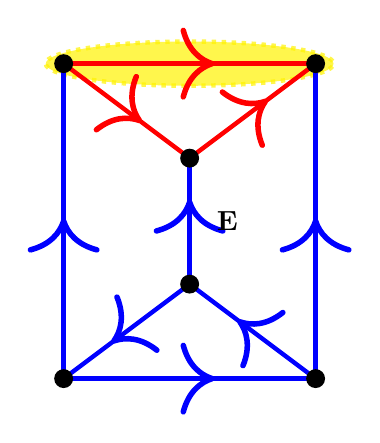
\begin{tikzpicture}[scale=0.8]
        \def\ver{0.15} %size of a vertex
        % v1
        \def\xa{0}
        \def\ya{0}
        % Highlight change
        \draw[fill=yellow, opacity=.7, ultra thick, dotted, rotate around={90:(\xa,\ya+1.5)},yellow] (\xa,\ya+1.5) ellipse (10pt and 65pt);
        % f_1 arrows
        \draw[middlearrow={>}, red] (\xa-2,\ya+1.5)-- (\xa+2,\ya+1.5);        % v2 - v3
        \draw[middlearrow={<}, red] (\xa+2,\ya+1.5) -- (\xa,\ya);             % v3 - v1
        \draw[middlearrow={<}, red] (\xa,\ya) -- (\xa-2,\ya+1.5);             % v1 - v2
        \draw[middlearrow={<}, blue] (\xa-2,\ya+1.5) -- (\xa-2,\ya-3.5);      % v2 - v4
        \draw[middlearrow={<}, blue] (\xa,\ya) -- (\xa,\ya-2);                % v1 - v6
        \draw[middlearrow={<}, blue] (\xa+2,\ya+1.5) -- (\xa+2,\ya-3.5);      % v3 - v5
        \draw[middlearrow={>}, blue] (\xa-2,\ya-3.5) -- (\xa+2,\ya-3.5);      % v4 - v5
        \draw[middlearrow={<}, blue] (\xa-2,\ya-3.5) -- (\xa,\ya-2);          % v4 - v6
        \draw[middlearrow={<}, blue] (\xa,\ya-2) -- (\xa+2,\ya-3.5);          % v6 - v5

        \draw[ultra thick, -, red] (\xa-2,\ya+1.5) -- (\xa+2,\ya+1.5);       % v2 - v3
        \draw[ultra thick, -, red] (\xa+2,\ya+1.5) -- (\xa,\ya);             % v3 - v1
        \draw[ultra thick, -, red] (\xa,\ya) -- (\xa-2,\ya+1.5);             % v1 - v2
        \draw[ultra thick, -, blue] (\xa-2,\ya+1.5) -- (\xa-2,\ya-3.5);      % v2 - v4
        \draw[ultra thick, -, blue] (\xa,\ya) -- (\xa,\ya-2);                % v1 - v6
        \draw[ultra thick, -, blue] (\xa+2,\ya+1.5) -- (\xa+2,\ya-3.5);      % v3 - v5
        \draw[ultra thick, -, blue] (\xa-2,\ya-3.5) -- (\xa+2,\ya-3.5);      % v4 - v5
        \draw[ultra thick, -, blue] (\xa-2,\ya-3.5) -- (\xa,\ya-2);          % v4 - v6
        \draw[ultra thick, -, blue] (\xa,\ya-2) -- (\xa+2,\ya-3.5);          % v6 - v5

        \node (a) at (\xa+0.6,\ya-1) {\textbf{E}};

        %graph G : Nodes fill
        \path[fill] (\xa,\ya) circle (\ver);           %v1
        \path[fill] (\xa-2,\ya+1.5) circle (\ver);   %v2
        \path[fill] (\xa+2,\ya+1.5) circle (\ver);   %v3
        \path[fill] (\xa-2,\ya-3.5) circle (\ver);   %v4
        \path[fill] (\xa+2,\ya-3.5) circle (\ver);   %v5
        \path[fill] (\xa,\ya-2) circle (\ver);         %v6
      \end{tikzpicture}
    \end{scaletikzpicturetowidth}
    \caption{$C_1$}
    \label{fig:input_instance_1}
  \end{subfigure}
  \begin{subfigure}[b]{0.4\textwidth}
    \begin{scaletikzpicturetowidth}{\textwidth}
      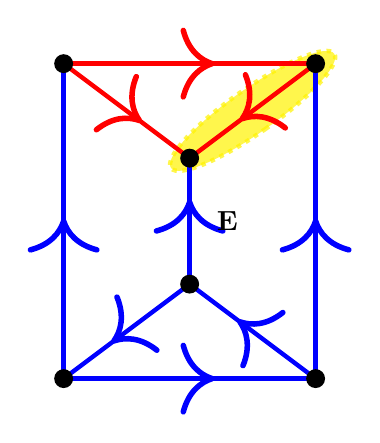
\begin{tikzpicture}[scale=0.8]
        \def\ver{0.15} %size of a vertex
        % v1
        \def\xa{0}
        \def\ya{0}
        % Highlight change
        \draw[fill=yellow, opacity=.7, ultra thick, dotted, rotate around={305:(\xa+1,\ya+0.75)},yellow] (\xa+1,\ya+0.75) ellipse (10pt and 45pt);
        % f_1 arrows
        \draw[middlearrow={>}, red] (\xa-2,\ya+1.5)-- (\xa+2,\ya+1.5);        % v2 - v3
        \draw[middlearrow={>}, red] (\xa+2,\ya+1.5) -- (\xa,\ya);             % v3 - v1
        \draw[middlearrow={<}, red] (\xa,\ya) -- (\xa-2,\ya+1.5);             % v1 - v2
        \draw[middlearrow={<}, blue] (\xa-2,\ya+1.5) -- (\xa-2,\ya-3.5);      % v2 - v4
        \draw[middlearrow={<}, blue] (\xa,\ya) -- (\xa,\ya-2);                % v1 - v6
        \draw[middlearrow={<}, blue] (\xa+2,\ya+1.5) -- (\xa+2,\ya-3.5);      % v3 - v5
        \draw[middlearrow={>}, blue] (\xa-2,\ya-3.5) -- (\xa+2,\ya-3.5);      % v4 - v5
        \draw[middlearrow={<}, blue] (\xa-2,\ya-3.5) -- (\xa,\ya-2);          % v4 - v6
        \draw[middlearrow={<}, blue] (\xa,\ya-2) -- (\xa+2,\ya-3.5);          % v6 - v5

        \draw[ultra thick, -, red] (\xa-2,\ya+1.5) -- (\xa+2,\ya+1.5);       % v2 - v3
        \draw[ultra thick, -, red] (\xa+2,\ya+1.5) -- (\xa,\ya);             % v3 - v1
        \draw[ultra thick, -, red] (\xa,\ya) -- (\xa-2,\ya+1.5);             % v1 - v2
        \draw[ultra thick, -, blue] (\xa-2,\ya+1.5) -- (\xa-2,\ya-3.5);      % v2 - v4
        \draw[ultra thick, -, blue] (\xa,\ya) -- (\xa,\ya-2);                % v1 - v6
        \draw[ultra thick, -, blue] (\xa+2,\ya+1.5) -- (\xa+2,\ya-3.5);      % v3 - v5
        \draw[ultra thick, -, blue] (\xa-2,\ya-3.5) -- (\xa+2,\ya-3.5);      % v4 - v5
        \draw[ultra thick, -, blue] (\xa-2,\ya-3.5) -- (\xa,\ya-2);          % v4 - v6
        \draw[ultra thick, -, blue] (\xa,\ya-2) -- (\xa+2,\ya-3.5);          % v6 - v5

        \node (a) at (\xa+0.6,\ya-1) {\textbf{E}};

        %graph G : Nodes fill
        \path[fill] (\xa,\ya) circle (\ver);           %v1
        \path[fill] (\xa-2,\ya+1.5) circle (\ver);   %v2
        \path[fill] (\xa+2,\ya+1.5) circle (\ver);   %v3
        \path[fill] (\xa-2,\ya-3.5) circle (\ver);   %v4
        \path[fill] (\xa+2,\ya-3.5) circle (\ver);   %v5
        \path[fill] (\xa,\ya-2) circle (\ver);         %v6
      \end{tikzpicture}
    \end{scaletikzpicturetowidth}
    \caption{$C_2$}
    \label{fig:input_instance_2}
  \end{subfigure}
  \begin{subfigure}[b]{0.4\textwidth}
    \begin{scaletikzpicturetowidth}{\textwidth}
      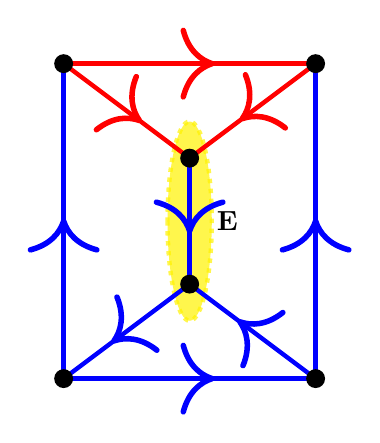
\begin{tikzpicture}[scale=0.8]
        \def\ver{0.15} %size of a vertex
        % v1
        \def\xa{0}
        \def\ya{0}
        % Highlight change
        \draw[fill=yellow, opacity=.7, ultra thick, dotted, rotate around={180:(\xa,\ya-1)},yellow] (\xa,\ya-1) ellipse (10pt and 45pt);
        % f_1 arrows
        \draw[middlearrow={>}, red] (\xa-2,\ya+1.5)-- (\xa+2,\ya+1.5);        % v2 - v3
        \draw[middlearrow={>}, red] (\xa+2,\ya+1.5) -- (\xa,\ya);             % v3 - v1
        \draw[middlearrow={<}, red] (\xa,\ya) -- (\xa-2,\ya+1.5);             % v1 - v2
        \draw[middlearrow={<}, blue] (\xa-2,\ya+1.5) -- (\xa-2,\ya-3.5);      % v2 - v4
        \draw[middlearrow={>}, blue] (\xa,\ya) -- (\xa,\ya-2);                % v1 - v6
        \draw[middlearrow={<}, blue] (\xa+2,\ya+1.5) -- (\xa+2,\ya-3.5);      % v3 - v5
        \draw[middlearrow={>}, blue] (\xa-2,\ya-3.5) -- (\xa+2,\ya-3.5);      % v4 - v5
        \draw[middlearrow={<}, blue] (\xa-2,\ya-3.5) -- (\xa,\ya-2);          % v4 - v6
        \draw[middlearrow={<}, blue] (\xa,\ya-2) -- (\xa+2,\ya-3.5);          % v6 - v5

        \draw[ultra thick, -, red] (\xa-2,\ya+1.5) -- (\xa+2,\ya+1.5);       % v2 - v3
        \draw[ultra thick, -, red] (\xa+2,\ya+1.5) -- (\xa,\ya);             % v3 - v1
        \draw[ultra thick, -, red] (\xa,\ya) -- (\xa-2,\ya+1.5);             % v1 - v2
        \draw[ultra thick, -, blue] (\xa-2,\ya+1.5) -- (\xa-2,\ya-3.5);      % v2 - v4
        \draw[ultra thick, -, blue] (\xa,\ya) -- (\xa,\ya-2);                % v1 - v6
        \draw[ultra thick, -, blue] (\xa+2,\ya+1.5) -- (\xa+2,\ya-3.5);      % v3 - v5
        \draw[ultra thick, -, blue] (\xa-2,\ya-3.5) -- (\xa+2,\ya-3.5);      % v4 - v5
        \draw[ultra thick, -, blue] (\xa-2,\ya-3.5) -- (\xa,\ya-2);          % v4 - v6
        \draw[ultra thick, -, blue] (\xa,\ya-2) -- (\xa+2,\ya-3.5);          % v6 - v5

        \node (a) at (\xa+0.6,\ya-1) {\textbf{E}};            % Label reject

        %graph G : Nodes fill
        \path[fill] (\xa,\ya) circle (\ver);           %v1
        \path[fill] (\xa-2,\ya+1.5) circle (\ver);   %v2
        \path[fill] (\xa+2,\ya+1.5) circle (\ver);   %v3
        \path[fill] (\xa-2,\ya-3.5) circle (\ver);   %v4
        \path[fill] (\xa+2,\ya-3.5) circle (\ver);   %v5
        \path[fill] (\xa,\ya-2) circle (\ver);         %v6
      \end{tikzpicture}
    \end{scaletikzpicturetowidth}
    \caption{$C_3$}
    \label{fig:input_instance_3}
  \end{subfigure}
  \caption{Reconfiguration sequence which transforms $C_0$ which is the initial configuration into $C_3 = $ which is the target configuration.}
  \label{fig:input_instance_config_to_edge}
\end{figure}

%%%%%%%%%%%%%%%%%%%%%%%%%%%%%%%%%%%%%%%%%%% Output instance %%%%%%%%%%%%%%%%%%%%%%%%%%%%%%%%
%------------------------------------------- out 1 & 2 ---------------------------------------------
\textbf{Output instance : SLIDING TOKEN instance.} \hfill

\begin{figure}[H]
  \raggedright
  \begin{subfigure}[b]{0.6\textwidth}
    \begin{scaletikzpicturetowidth}{\textwidth}
      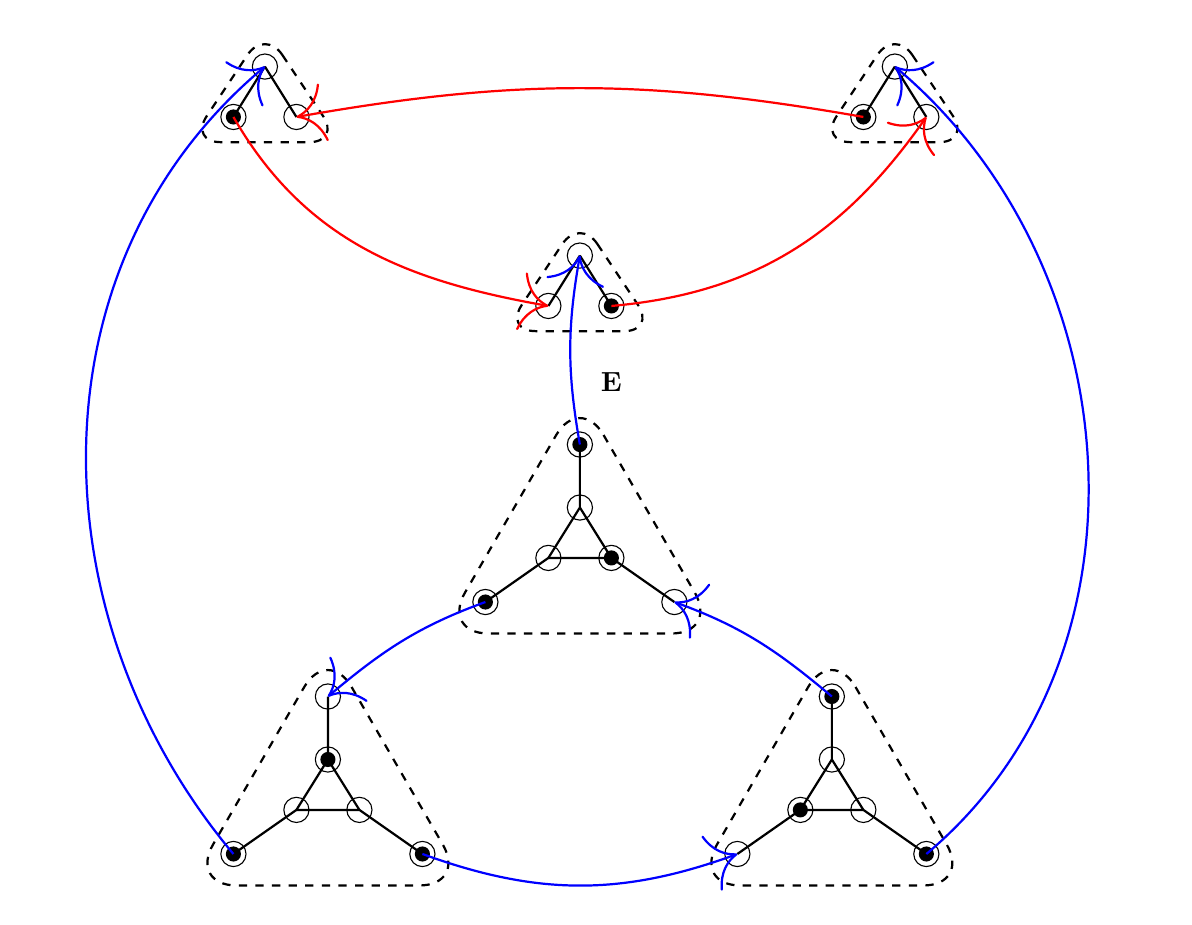
\begin{tikzpicture}[scale=0.8]
        %%%%%%%%%%%% AND 1 %%%%%%%%%%%%
        \def\ver{0.12} %size of a vertex
        \def\xa{-1}
        \def\ya{0}
        % Highlight change
        %graph G
        \draw (\xa,\ya) circle (0.2cm);          %v1 no fill
        \draw (\xa+0.5,\ya-0.8) circle (0.2cm);  %v4 no fill
        \draw (\xa-0.5,\ya-0.8) circle (0.2cm);  %v3 no fill
        % Tokens
        \path[fill] (\xa-0.5,\ya-0.8) circle (\ver);   %v3
        %labels
        \draw[thick] (\xa,\ya)--(\xa-0.5,\ya-0.8);
        \draw[thick] (\xa,\ya)--(\xa+0.5,\ya-0.8);
        \path[draw, thick, dashed, rounded corners=4mm] (\xa,\ya+0.6)--(\xa+1.2,\ya-1.2)--(\xa-1.2,\ya-1.2)--cycle;
        %%%%%%%%%%%% AND 2 %%%%%%%%%%%%
        \def\ver{0.12} %size of a vertex
        \def\xb{4}
        \def\yb{-3}
        %graph G
        \draw (\xb,\yb) circle (0.2cm);          %v1 no fill
        \draw (\xb+0.5,\yb-0.8) circle (0.2cm);  %v4 no fill
        \draw (\xb-0.5,\yb-0.8) circle (0.2cm);  %v3 no fill
        % Tokens
        \path[fill] (\xb+0.5,\yb-0.8) circle (\ver);   %v3
        %labels
        \draw[thick] (\xb,\yb)--(\xb-0.5,\yb-0.8);
        \draw[thick] (\xb,\yb)--(\xb+0.5,\yb-0.8);
        \path[draw, thick, dashed, rounded corners=4mm] (\xb,\yb+0.6)--(\xb+1.2,\yb-1.2)--(\xb-1.2,\yb-1.2)--cycle;
        %%%%%%%%%%%% AND 3 %%%%%%%%%%%%
        \def\ver{0.12} %size of a vertex
        \def\xc{9}
        \def\yc{0}
        %graph G
        \draw (\xc,\yc) circle (0.2cm);          %v1 no fill
        \draw (\xc+0.5,\yc-0.8) circle (0.2cm);  %v4 no fill
        \draw (\xc-0.5,\yc-0.8) circle (0.2cm);  %v3 no fill
        % Tokens
        \path[fill] (\xc-0.5,\yc-0.8) circle (\ver);   %v3
        %labels
        \draw[thick] (\xc,\yc)--(\xc-0.5,\yc-0.8);
        \draw[thick] (\xc,\yc)--(\xc+0.5,\yc-0.8);
        \path[draw, thick, dashed, rounded corners=4mm] (\xc,\yc+0.6)--(\xc+1.2,\yc-1.2)--(\xc-1.2,\yc-1.2)--cycle;
        %%%%%%%%%%%% OR 1 %%%%%%%%%%%%
        \def\ver{0.12} %size of a vertex
        \def\xd{0}
        \def\yd{-11}
        %G_1
        \draw (\xd,\yd) circle (0.2cm);           %v1
        \draw (\xd+0.5,\yd-0.8) circle (0.2cm);   %v4
        \draw (\xd-0.5,\yd-0.8) circle (0.2cm);   %v3
        \draw (\xd,\yd+1) circle (0.2cm);         %v2
        \draw (\xd-1.5,\yd-1.5) circle (0.2cm);   %v5
        \draw (\xd+1.5,\yd-1.5) circle (0.2cm);   %v6
        \path[fill] (\xd,\yd) circle (\ver);           %v1
        \path[fill] (\xd-1.5,\yd-1.5) circle (\ver);   %v5
        \path[fill] (\xd+1.5,\yd-1.5) circle (\ver);   %v6
        %labels
        \draw[thick] (\xd,\yd+1)--(\xd, \yd)--(\xd-0.5,\yd-0.8)--(\xd-1.5,\yd-1.5);
        \draw[thick] (\xd-0.5,\yd-0.8)--(\xd+0.5,\yd-0.8)--(\xd+1.5,\yd-1.5);
        \draw[thick] (\xd,\yd)-- (\xd+0.5,\yd-0.8);

        \path[draw, thick, dashed, rounded corners=6mm] (\xd,\yd+1.8)--(\xd+2.2,\yd-2)--(\xd-2.2,\yd-2)--cycle;
        %%%%%%%%%%%% OR 2 %%%%%%%%%%%%
        \def\ver{0.12} %size of a vertex
        \def\xe{4}
        \def\ye{-7}
        %G_1
        \draw (\xe,\ye) circle (0.2cm);           %v1
        \draw (\xe+0.5,\ye-0.8) circle (0.2cm);   %v4
        \draw (\xe-0.5,\ye-0.8) circle (0.2cm);   %v3
        \draw (\xe,\ye+1) circle (0.2cm);         %v2
        \draw (\xe-1.5,\ye-1.5) circle (0.2cm);   %v5
        \draw (\xe+1.5,\ye-1.5) circle (0.2cm);   %v6

        \path[fill] (\xe,\ye+1) circle (\ver);         %v2
        \path[fill] (\xe+0.5,\ye-0.8) circle (\ver);   %v4
        \path[fill] (\xe-1.5,\ye-1.5) circle (\ver);   %v5
        %labels
        \draw[thick] (\xe,\ye+1)--(\xe, \ye)--(\xe-0.5,\ye-0.8)--(\xe-1.5,\ye-1.5);
        \draw[thick] (\xe-0.5,\ye-0.8)--(\xe+0.5,\ye-0.8)--(\xe+1.5,\ye-1.5);
        \draw[thick] (\xe,\ye)-- (\xe+0.5,\ye-0.8);
        \path[draw, thick, dashed, rounded corners=6mm] (\xe,\ye+1.8)--(\xe+2.2,\ye-2)--(\xe-2.2,\ye-2)--cycle;
        %%%%%%%%%%%% OR 3 %%%%%%%%%%%%
        \def\ver{0.12} %size of a vertex
        \def\xf{8}
        \def\yf{-11}
        %G_1
        \draw (\xf,\yf) circle (0.2cm);           %v1
        \draw (\xf+0.5,\yf-0.8) circle (0.2cm);   %v4
        \draw (\xf-0.5,\yf-0.8) circle (0.2cm);   %v3
        \draw (\xf,\yf+1) circle (0.2cm);         %v2
        \draw (\xf-1.5,\yf-1.5) circle (0.2cm);   %v5
        \draw (\xf+1.5,\yf-1.5) circle (0.2cm);   %v6

        \path[fill] (\xf,\yf+1) circle (\ver);         %v2
        \path[fill] (\xf-0.5,\yf-0.8) circle (\ver);   %v3
        \path[fill] (\xf+1.5,\yf-1.5) circle (\ver);   %v6
        %labels
        \draw[thick] (\xf,\yf+1)--(\xf, \yf)--(\xf-0.5,\yf-0.8)--(\xf-1.5,\yf-1.5);
        \draw[thick] (\xf-0.5,\yf-0.8)--(\xf+0.5,\yf-0.8)--(\xf+1.5,\yf-1.5);
        \draw[thick] (\xf,\yf)-- (\xf+0.5,\yf-0.8);
        \path[draw, thick, dashed, rounded corners=6mm] (\xf,\yf+1.8)--(\xf+2.2,\yf-2)--(\xf-2.2,\yf-2)--cycle;
        %%%%%%%%%%% EDGES %%%%%%%%%
        \node (a) at (4.5,-5) {\textbf{E}};            % Label reject
        \draw [-, red, thick, arrows={->[scale=3,red]}] (\xc-0.5,\yc-0.8) to [out=170,in=10] (\xa+0.5,\ya-0.8);            % AND 3  -- AND 1
        \draw [-, red, thick, arrows={->[scale=3,red]}] (\xa-0.5,\ya-0.8)  to [out=300,in=170] (\xb-0.5,\yb-0.8);          % AND 1  -- AND 2
        \draw [-, red, thick, arrows={->[scale=3,red]}] (\xb+0.5,\yb-0.8) to [out=5,in=235] (\xc+0.5,\yc-0.8);             % AND 2  -- AND 3
        \draw [-, blue, thick, arrows={->[scale=3,blue]}] (\xd-1.5,\yd-1.5) to [out=130,in=220] (\xa,\ya);                 % OR 1  -- AND 1
        \draw [-, blue, thick, arrows={->[scale=3,blue]}] (\xd+1.5,\yd-1.5) to [out=340,in=200] (\xf-1.5,\yf-1.5);         % OR 1  -- OR 3
        \draw [-, blue, thick, arrows={->[scale=3,blue]}] (\xf,\yf+1)  to [out=140,in=340] (\xe+1.5,\ye-1.5);              % OR 3  -- OR 2
        \draw [-, blue, thick, arrows={->[scale=3,blue]}] (\xe-1.5,\ye-1.5) to [out=200,in=40] (\xd,\yd+1);                % OR 2  -- OR 1
        \draw [-, blue, thick, arrows={->[scale=3,blue]}] (\xf+1.5,\yf-1.5) to [out=40,in=320] (\xc,\yc);                  % OR 3  -- AND 3
        \draw [-, blue, thick, arrows={->[scale=3,blue]}] (\xe,\ye+1) to [out=100,in=260] (\xb,\yb);                       % OR 2  -- AND 2
      \end{tikzpicture}
    \end{scaletikzpicturetowidth}
  \caption{$S_0$.}
  \label{fig:output_instance_final}
  \end{subfigure}
  \vspace{3em}
  \begin{subfigure}[b]{0.6\textwidth}
    \begin{scaletikzpicturetowidth}{\textwidth}
      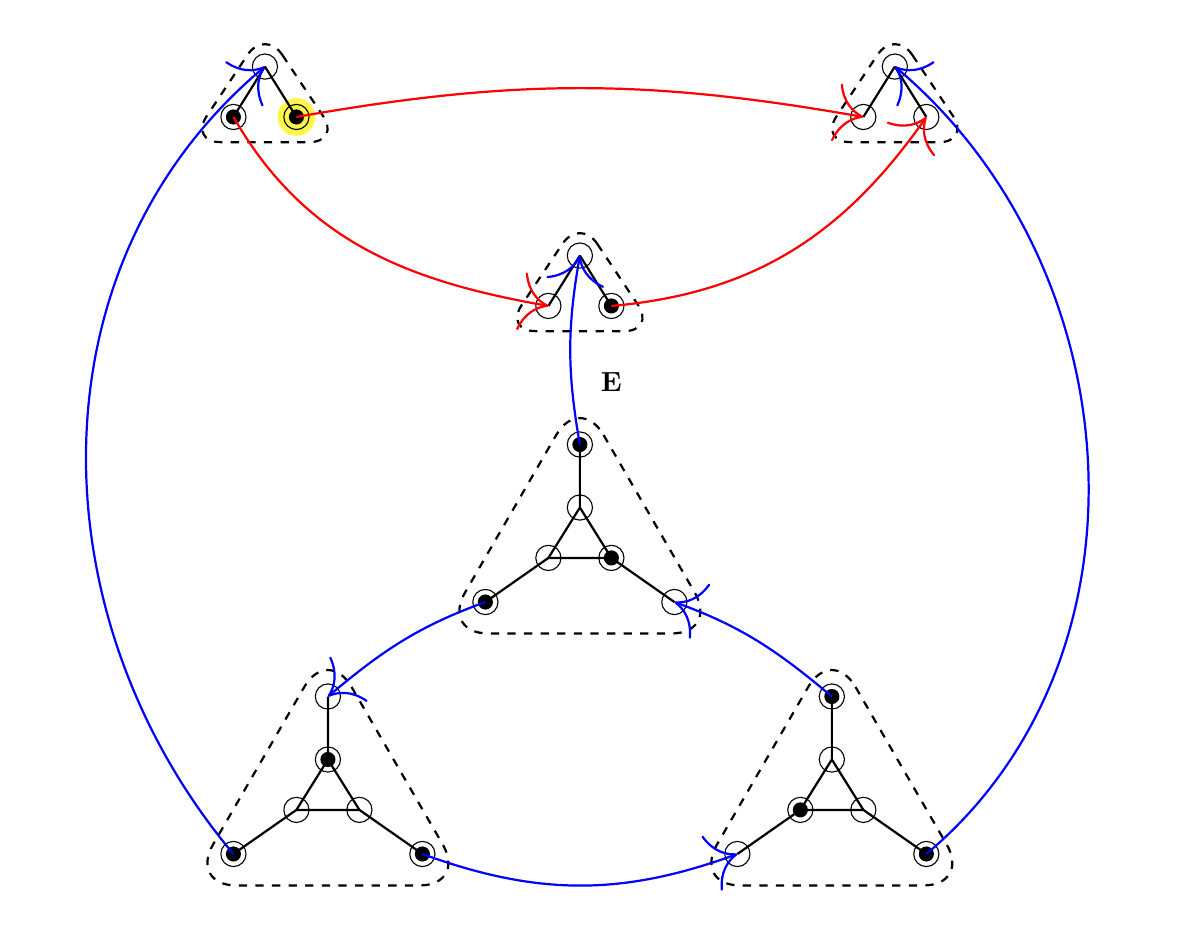
\begin{tikzpicture}[scale=0.8]
        %%%%%%%%%%%% AND 1 %%%%%%%%%%%%
        \def\ver{0.12} %size of a vertex
        \def\xa{-1}
        \def\ya{0}
        % Highlight change
        \draw[fill=yellow, opacity=.7, draw=none] (\xa+0.5,\ya-0.8) circle (0.3cm);
        %\draw[fill=yellow, opacity=.7, draw=none] (\xa-0.5,\ya-0.8) circle (0.3cm);
        %graph G
        \draw (\xa,\ya) circle (0.2cm);          %v1 no fill
        \draw (\xa+0.5,\ya-0.8) circle (0.2cm);  %v4 no fill
        \draw (\xa-0.5,\ya-0.8) circle (0.2cm);  %v3 no fill
        % Tokens
        \path[fill] (\xa-0.5,\ya-0.8) circle (\ver);   %v3
        \path[fill] (\xa+0.5,\ya-0.8) circle (\ver);   %v4
        %labels
        \draw[thick] (\xa,\ya)--(\xa-0.5,\ya-0.8);
        \draw[thick] (\xa,\ya)--(\xa+0.5,\ya-0.8);
        \path[draw, thick, dashed, rounded corners=4mm] (\xa,\ya+0.6)--(\xa+1.2,\ya-1.2)--(\xa-1.2,\ya-1.2)--cycle;
        %%%%%%%%%%%% AND 2 %%%%%%%%%%%%
        \def\ver{0.12} %size of a vertex
        \def\xb{4}
        \def\yb{-3}
        %graph G
        \draw (\xb,\yb) circle (0.2cm);          %v1 no fill
        \draw (\xb+0.5,\yb-0.8) circle (0.2cm);  %v4 no fill
        \draw (\xb-0.5,\yb-0.8) circle (0.2cm);  %v3 no fill
        % Tokens
        \path[fill] (\xb+0.5,\yb-0.8) circle (\ver);   %v3
        %labels
        \draw[thick] (\xb,\yb)--(\xb-0.5,\yb-0.8);
        \draw[thick] (\xb,\yb)--(\xb+0.5,\yb-0.8);
        \path[draw, thick, dashed, rounded corners=4mm] (\xb,\yb+0.6)--(\xb+1.2,\yb-1.2)--(\xb-1.2,\yb-1.2)--cycle;
        %%%%%%%%%%%% AND 3 %%%%%%%%%%%%
        \def\ver{0.12} %size of a vertex
        \def\xc{9}
        \def\yc{0}
        %graph G
        \draw (\xc,\yc) circle (0.2cm);          %v1 no fill
        \draw (\xc+0.5,\yc-0.8) circle (0.2cm);  %v4 no fill
        \draw (\xc-0.5,\yc-0.8) circle (0.2cm);  %v3 no fill
        %labels
        \draw[thick] (\xc,\yc)--(\xc-0.5,\yc-0.8);
        \draw[thick] (\xc,\yc)--(\xc+0.5,\yc-0.8);
        \path[draw, thick, dashed, rounded corners=4mm] (\xc,\yc+0.6)--(\xc+1.2,\yc-1.2)--(\xc-1.2,\yc-1.2)--cycle;
        %%%%%%%%%%%% OR 1 %%%%%%%%%%%%
        \def\ver{0.12} %size of a vertex
        \def\xd{0}
        \def\yd{-11}
        %G_1
        \draw (\xd,\yd) circle (0.2cm);           %v1
        \draw (\xd+0.5,\yd-0.8) circle (0.2cm);   %v4
        \draw (\xd-0.5,\yd-0.8) circle (0.2cm);   %v3
        \draw (\xd,\yd+1) circle (0.2cm);         %v2
        \draw (\xd-1.5,\yd-1.5) circle (0.2cm);   %v5
        \draw (\xd+1.5,\yd-1.5) circle (0.2cm);   %v6

        \path[fill] (\xd,\yd) circle (\ver);           %v1
        \path[fill] (\xd-1.5,\yd-1.5) circle (\ver);   %v5
        \path[fill] (\xd+1.5,\yd-1.5) circle (\ver);   %v6
        %labels
        \draw[thick] (\xd,\yd+1)--(\xd, \yd)--(\xd-0.5,\yd-0.8)--(\xd-1.5,\yd-1.5);
        \draw[thick] (\xd-0.5,\yd-0.8)--(\xd+0.5,\yd-0.8)--(\xd+1.5,\yd-1.5);
        \draw[thick] (\xd,\yd)-- (\xd+0.5,\yd-0.8);
        \path[draw, thick, dashed, rounded corners=6mm] (\xd,\yd+1.8)--(\xd+2.2,\yd-2)--(\xd-2.2,\yd-2)--cycle;
        %%%%%%%%%%%% OR 2 %%%%%%%%%%%%
        \def\ver{0.12} %size of a vertex
        \def\xe{4}
        \def\ye{-7}
        %G_1
        \draw (\xe,\ye) circle (0.2cm);           %v1
        \draw (\xe+0.5,\ye-0.8) circle (0.2cm);   %v4
        \draw (\xe-0.5,\ye-0.8) circle (0.2cm);   %v3
        \draw (\xe,\ye+1) circle (0.2cm);         %v2
        \draw (\xe-1.5,\ye-1.5) circle (0.2cm);   %v5
        \draw (\xe+1.5,\ye-1.5) circle (0.2cm);   %v6
        \path[fill] (\xe,\ye+1) circle (\ver);         %v2
        \path[fill] (\xe+0.5,\ye-0.8) circle (\ver);   %v4
        \path[fill] (\xe-1.5,\ye-1.5) circle (\ver);   %v5
        %labels
        \draw[thick] (\xe,\ye+1)--(\xe, \ye)--(\xe-0.5,\ye-0.8)--(\xe-1.5,\ye-1.5);
        \draw[thick] (\xe-0.5,\ye-0.8)--(\xe+0.5,\ye-0.8)--(\xe+1.5,\ye-1.5);
        \draw[thick] (\xe,\ye)-- (\xe+0.5,\ye-0.8);
        \path[draw, thick, dashed, rounded corners=6mm] (\xe,\ye+1.8)--(\xe+2.2,\ye-2)--(\xe-2.2,\ye-2)--cycle;
        %%%%%%%%%%%% OR 3 %%%%%%%%%%%%
        \def\ver{0.12} %size of a vertex
        \def\xf{8}
        \def\yf{-11}
        %G_1
        \draw (\xf,\yf) circle (0.2cm);           %v1
        \draw (\xf+0.5,\yf-0.8) circle (0.2cm);   %v4
        \draw (\xf-0.5,\yf-0.8) circle (0.2cm);   %v3
        \draw (\xf,\yf+1) circle (0.2cm);         %v2
        \draw (\xf-1.5,\yf-1.5) circle (0.2cm);   %v5
        \draw (\xf+1.5,\yf-1.5) circle (0.2cm);   %v6
        %tokens
        \path[fill] (\xf,\yf+1) circle (\ver);         %v2
        \path[fill] (\xf-0.5,\yf-0.8) circle (\ver);   %v3
        \path[fill] (\xf+1.5,\yf-1.5) circle (\ver);   %v6
        %labels
        \draw[thick] (\xf,\yf+1)--(\xf, \yf)--(\xf-0.5,\yf-0.8)--(\xf-1.5,\yf-1.5);
        \draw[thick] (\xf-0.5,\yf-0.8)--(\xf+0.5,\yf-0.8)--(\xf+1.5,\yf-1.5);
        \draw[thick] (\xf,\yf)-- (\xf+0.5,\yf-0.8);
        \path[draw, thick, dashed, rounded corners=6mm] (\xf,\yf+1.8)--(\xf+2.2,\yf-2)--(\xf-2.2,\yf-2)--cycle;
        %%%%%%%%%%% EDGES %%%%%%%%%
        \node (a) at (4.5,-5) {\textbf{E}};            % Label reject
        \draw [-, red, thick, arrows={->[scale=3,red]}]  (\xa+0.5,\ya-0.8) to [out=10,in=170]  (\xc-0.5,\yc-0.8);          % AND 1  -- AND 3
        \draw [-, red, thick, arrows={->[scale=3,red]}] (\xa-0.5,\ya-0.8)  to [out=300,in=170] (\xb-0.5,\yb-0.8);          % AND 1  -- AND 2
        \draw [-, red, thick, arrows={->[scale=3,red]}] (\xb+0.5,\yb-0.8) to [out=5,in=235] (\xc+0.5,\yc-0.8);             % AND 2  -- AND 3
        \draw [-, blue, thick, arrows={->[scale=3,blue]}] (\xd-1.5,\yd-1.5) to [out=130,in=220] (\xa,\ya);                 % OR 1  -- AND 1
        \draw [-, blue, thick, arrows={->[scale=3,blue]}] (\xd+1.5,\yd-1.5) to [out=340,in=200] (\xf-1.5,\yf-1.5);         % OR 1  -- OR 3
        \draw [-, blue, thick, arrows={->[scale=3,blue]}] (\xf,\yf+1)  to [out=140,in=340] (\xe+1.5,\ye-1.5);              % OR 3  -- OR 2
        \draw [-, blue, thick, arrows={->[scale=3,blue]}] (\xe-1.5,\ye-1.5) to [out=200,in=40] (\xd,\yd+1);                % OR 2  -- OR 1
        \draw [-, blue, thick, arrows={->[scale=3,blue]}] (\xf+1.5,\yf-1.5) to [out=40,in=320] (\xc,\yc);                  % OR 3  -- AND 3
        \draw [-, blue, thick, arrows={->[scale=3,blue]}] (\xe,\ye+1) to [out=100,in=260] (\xb,\yb);                       % OR 2  -- AND 2
      \end{tikzpicture}
    \end{scaletikzpicturetowidth}
    \caption{$S_1.$}
    \label{fig:output_instance_final}
  \end{subfigure}
\end{figure}


%------------------------------------------- out 3 & 4 ---------------------------------------------
\begin{figure}[H]\ContinuedFloat
  \raggedright
  \begin{subfigure}[b]{0.6\textwidth}
    \begin{scaletikzpicturetowidth}{\textwidth}
      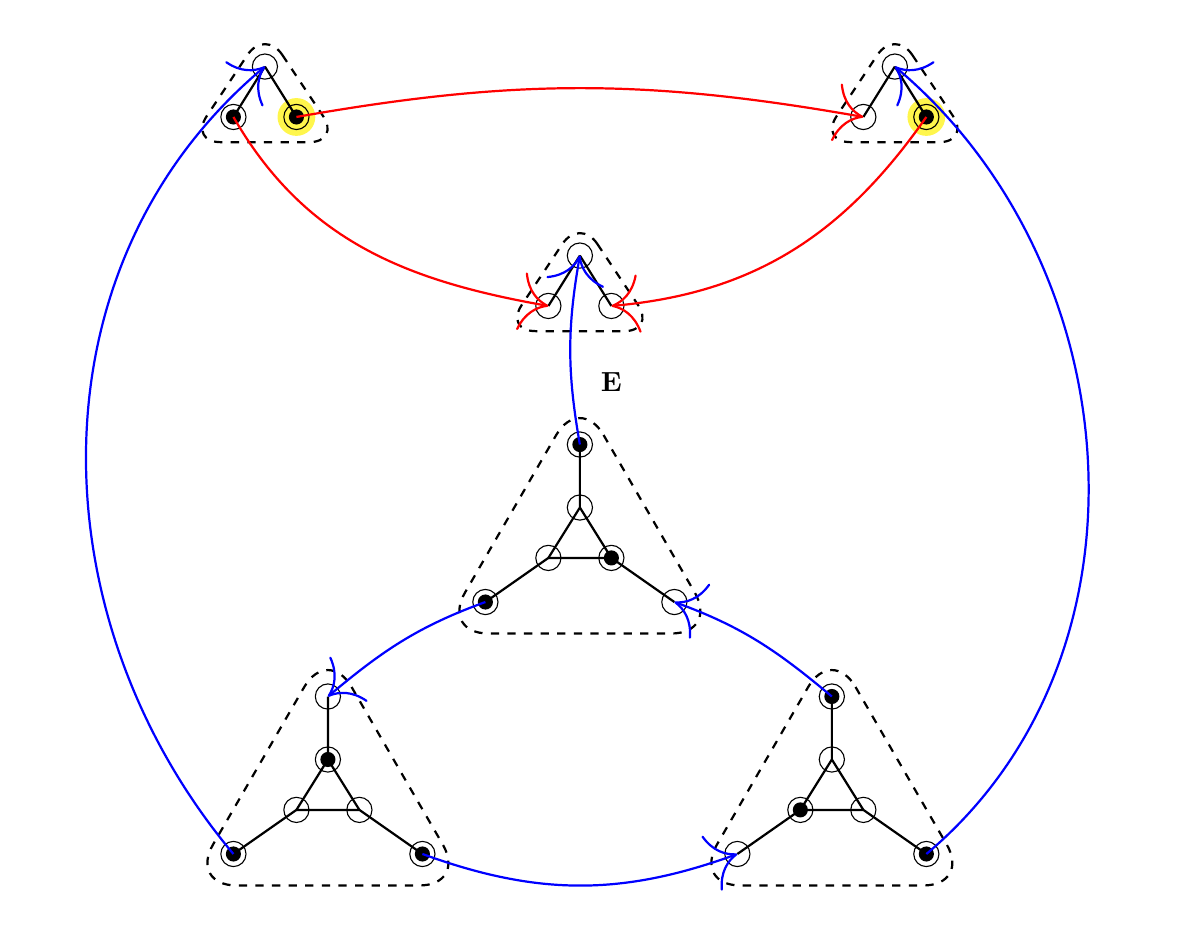
\begin{tikzpicture}[scale=0.8]
        %%%%%%%%%%%% AND 1 %%%%%%%%%%%%
        \def\ver{0.12} %size of a vertex
        \def\xa{-1}
        \def\ya{0}
        % Highlight change
        \draw[fill=yellow, opacity=.7, draw=none] (\xa+0.5,\ya-0.8) circle (0.3cm);
        %\draw[fill=yellow, opacity=.7, draw=none] (\xa-0.5,\ya-0.8) circle (0.3cm);
        %graph G
        \draw (\xa,\ya) circle (0.2cm);          %v1 no fill
        \draw (\xa+0.5,\ya-0.8) circle (0.2cm);  %v4 no fill
        \draw (\xa-0.5,\ya-0.8) circle (0.2cm);  %v3 no fill
        % Tokens
        \path[fill] (\xa-0.5,\ya-0.8) circle (\ver);   %v3
        \path[fill] (\xa+0.5,\ya-0.8) circle (\ver);   %v4
        %labels
        \draw[thick] (\xa,\ya)--(\xa-0.5,\ya-0.8);
        \draw[thick] (\xa,\ya)--(\xa+0.5,\ya-0.8);
        \path[draw, thick, dashed, rounded corners=4mm] (\xa,\ya+0.6)--(\xa+1.2,\ya-1.2)--(\xa-1.2,\ya-1.2)--cycle;
        %%%%%%%%%%%% AND 2 %%%%%%%%%%%%
        \def\ver{0.12} %size of a vertex
        \def\xb{4}
        \def\yb{-3}
        %graph G
        \draw (\xb,\yb) circle (0.2cm);          %v1 no fill
        \draw (\xb+0.5,\yb-0.8) circle (0.2cm);  %v4 no fill
        \draw (\xb-0.5,\yb-0.8) circle (0.2cm);  %v3 no fill
        %labels
        \draw[thick] (\xb,\yb)--(\xb-0.5,\yb-0.8);
        \draw[thick] (\xb,\yb)--(\xb+0.5,\yb-0.8);
        \path[draw, thick, dashed, rounded corners=4mm] (\xb,\yb+0.6)--(\xb+1.2,\yb-1.2)--(\xb-1.2,\yb-1.2)--cycle;
        %%%%%%%%%%%% AND 3 %%%%%%%%%%%%
        \def\ver{0.12} %size of a vertex
        \def\xc{9}
        \def\yc{0}
        % Highlight
        \draw[fill=yellow, opacity=.7, draw=none] (\xc+0.5,\yc-0.8) circle (0.3cm);
        %graph G
        \draw (\xc,\yc) circle (0.2cm);          %v1 no fill
        \draw (\xc+0.5,\yc-0.8) circle (0.2cm);  %v4 no fill
        \draw (\xc-0.5,\yc-0.8) circle (0.2cm);  %v3 no fill
        % Tokens
        \path[fill] (\xc+0.5,\yc-0.8) circle (\ver);   %v4
        %labels
        \draw[thick] (\xc,\yc)--(\xc-0.5,\yc-0.8);
        \draw[thick] (\xc,\yc)--(\xc+0.5,\yc-0.8);
        \path[draw, thick, dashed, rounded corners=4mm] (\xc,\yc+0.6)--(\xc+1.2,\yc-1.2)--(\xc-1.2,\yc-1.2)--cycle;
        %%%%%%%%%%%% OR 1 %%%%%%%%%%%%
        \def\ver{0.12} %size of a vertex
        \def\xd{0}
        \def\yd{-11}
        %G_1
        \draw (\xd,\yd) circle (0.2cm);           %v1
        \draw (\xd+0.5,\yd-0.8) circle (0.2cm);   %v4
        \draw (\xd-0.5,\yd-0.8) circle (0.2cm);   %v3
        \draw (\xd,\yd+1) circle (0.2cm);         %v2
        \draw (\xd-1.5,\yd-1.5) circle (0.2cm);   %v5
        \draw (\xd+1.5,\yd-1.5) circle (0.2cm);   %v6
        % tokens
        \path[fill] (\xd,\yd) circle (\ver);           %v1
        \path[fill] (\xd-1.5,\yd-1.5) circle (\ver);   %v5
        \path[fill] (\xd+1.5,\yd-1.5) circle (\ver);   %v6
        %labels
        \draw[thick] (\xd,\yd+1)--(\xd, \yd)--(\xd-0.5,\yd-0.8)--(\xd-1.5,\yd-1.5);
        \draw[thick] (\xd-0.5,\yd-0.8)--(\xd+0.5,\yd-0.8)--(\xd+1.5,\yd-1.5);
        \draw[thick] (\xd,\yd)-- (\xd+0.5,\yd-0.8);
        %edges
        \path[draw, thick, dashed, rounded corners=6mm] (\xd,\yd+1.8)--(\xd+2.2,\yd-2)--(\xd-2.2,\yd-2)--cycle;
        %%%%%%%%%%%% OR 2 %%%%%%%%%%%%
        \def\ver{0.12} %size of a vertex
        \def\xe{4}
        \def\ye{-7}
        %G_1
        \draw (\xe,\ye) circle (0.2cm);           %v1
        \draw (\xe+0.5,\ye-0.8) circle (0.2cm);   %v4
        \draw (\xe-0.5,\ye-0.8) circle (0.2cm);   %v3
        \draw (\xe,\ye+1) circle (0.2cm);         %v2
        \draw (\xe-1.5,\ye-1.5) circle (0.2cm);   %v5
        \draw (\xe+1.5,\ye-1.5) circle (0.2cm);   %v6
        % token
        \path[fill] (\xe,\ye+1) circle (\ver);         %v2
        \path[fill] (\xe+0.5,\ye-0.8) circle (\ver);   %v4
        \path[fill] (\xe-1.5,\ye-1.5) circle (\ver);   %v5
        %labels
        \draw[thick] (\xe,\ye+1)--(\xe, \ye)--(\xe-0.5,\ye-0.8)--(\xe-1.5,\ye-1.5);
        \draw[thick] (\xe-0.5,\ye-0.8)--(\xe+0.5,\ye-0.8)--(\xe+1.5,\ye-1.5);
        \draw[thick] (\xe,\ye)-- (\xe+0.5,\ye-0.8);

        \path[draw, thick, dashed, rounded corners=6mm] (\xe,\ye+1.8)--(\xe+2.2,\ye-2)--(\xe-2.2,\ye-2)--cycle;

        %%%%%%%%%%%% OR 3 %%%%%%%%%%%%
        \def\ver{0.12} %size of a vertex
        \def\xf{8}
        \def\yf{-11}
        %G_1
        \draw (\xf,\yf) circle (0.2cm);           %v1
        \draw (\xf+0.5,\yf-0.8) circle (0.2cm);   %v4
        \draw (\xf-0.5,\yf-0.8) circle (0.2cm);   %v3
        \draw (\xf,\yf+1) circle (0.2cm);         %v2
        \draw (\xf-1.5,\yf-1.5) circle (0.2cm);   %v5
        \draw (\xf+1.5,\yf-1.5) circle (0.2cm);   %v6

        \path[fill] (\xf,\yf+1) circle (\ver);         %v2
        \path[fill] (\xf-0.5,\yf-0.8) circle (\ver);   %v3
        \path[fill] (\xf+1.5,\yf-1.5) circle (\ver);   %v6
        %labels
        \draw[thick] (\xf,\yf+1)--(\xf, \yf)--(\xf-0.5,\yf-0.8)--(\xf-1.5,\yf-1.5);
        \draw[thick] (\xf-0.5,\yf-0.8)--(\xf+0.5,\yf-0.8)--(\xf+1.5,\yf-1.5);
        \draw[thick] (\xf,\yf)-- (\xf+0.5,\yf-0.8);

        \path[draw, thick, dashed, rounded corners=6mm] (\xf,\yf+1.8)--(\xf+2.2,\yf-2)--(\xf-2.2,\yf-2)--cycle;
        %%%%%%%%%%% EDGES %%%%%%%%%
        \node (a) at (4.5,-5) {\textbf{E}};            % Label reject
        \draw [-, red, thick, arrows={->[scale=3,red]}]  (\xa+0.5,\ya-0.8) to [out=10,in=170]  (\xc-0.5,\yc-0.8);          % AND 1  -- AND 3
        \draw [-, red, thick, arrows={->[scale=3,red]}] (\xa-0.5,\ya-0.8)  to [out=300,in=170] (\xb-0.5,\yb-0.8);          % AND 1  -- AND 2
        \draw [-, red, thick, arrows={->[scale=3,red]}] (\xc+0.5,\yc-0.8) to [out=235,in=5] (\xb+0.5,\yb-0.8) ;            % AND 3  -- AND 2
        \draw [-, blue, thick, arrows={->[scale=3,blue]}] (\xd-1.5,\yd-1.5) to [out=130,in=220] (\xa,\ya);                 % OR 1  -- AND 1
        \draw [-, blue, thick, arrows={->[scale=3,blue]}] (\xd+1.5,\yd-1.5) to [out=340,in=200] (\xf-1.5,\yf-1.5);         % OR 1  -- OR 3
        \draw [-, blue, thick, arrows={->[scale=3,blue]}] (\xf,\yf+1)  to [out=140,in=340] (\xe+1.5,\ye-1.5);              % OR 3  -- OR 2
        \draw [-, blue, thick, arrows={->[scale=3,blue]}] (\xe-1.5,\ye-1.5) to [out=200,in=40] (\xd,\yd+1);                % OR 2  -- OR 1
        \draw [-, blue, thick, arrows={->[scale=3,blue]}] (\xf+1.5,\yf-1.5) to [out=40,in=320] (\xc,\yc);                  % OR 3  -- AND 3
        \draw [-, blue, thick, arrows={->[scale=3,blue]}] (\xe,\ye+1) to [out=100,in=260] (\xb,\yb);                       % OR 2  -- AND 2
      \end{tikzpicture}
    \end{scaletikzpicturetowidth}
    \caption{$S_2.$}
    \label{fig:output_instance_final}
  \end{subfigure}
  \vspace{3em}
  \begin{subfigure}[b]{0.6\textwidth}
    \begin{scaletikzpicturetowidth}{\textwidth}
      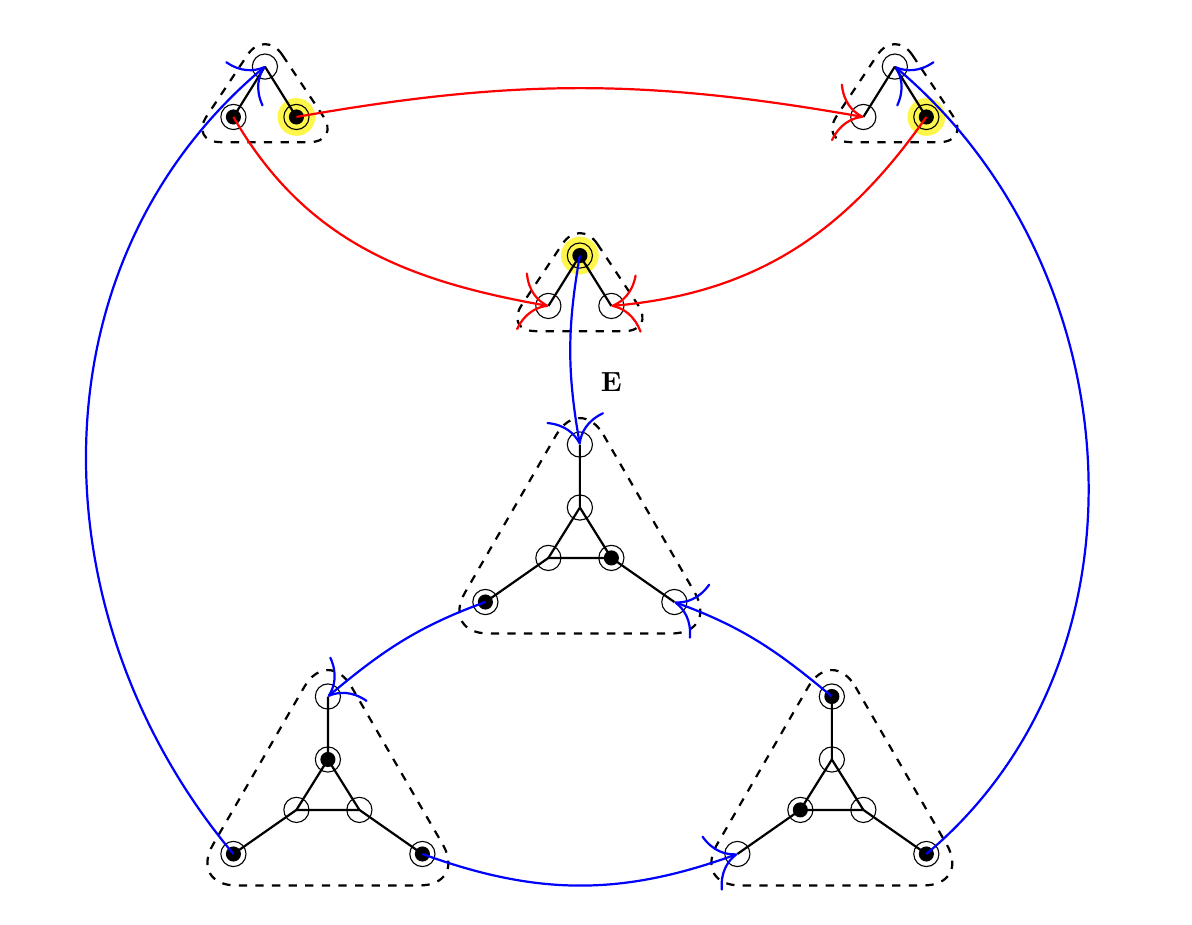
\begin{tikzpicture}[scale=0.8]
        %%%%%%%%%%%% AND 1 %%%%%%%%%%%%
        \def\ver{0.12} %size of a vertex
        \def\xa{-1}
        \def\ya{0}
        % Highlight change
        \draw[fill=yellow, opacity=.7, draw=none] (\xa+0.5,\ya-0.8) circle (0.3cm);
        %\draw[fill=yellow, opacity=.7, draw=none] (\xa-0.5,\ya-0.8) circle (0.3cm);
        %graph G
        \draw (\xa,\ya) circle (0.2cm);          %v1 no fill
        \draw (\xa+0.5,\ya-0.8) circle (0.2cm);  %v4 no fill
        \draw (\xa-0.5,\ya-0.8) circle (0.2cm);  %v3 no fill
        % Tokens
        \path[fill] (\xa-0.5,\ya-0.8) circle (\ver);   %v3
        \path[fill] (\xa+0.5,\ya-0.8) circle (\ver);   %v4
        %labels
        \draw[thick] (\xa,\ya)--(\xa-0.5,\ya-0.8);
        \draw[thick] (\xa,\ya)--(\xa+0.5,\ya-0.8);
        \path[draw, thick, dashed, rounded corners=4mm] (\xa,\ya+0.6)--(\xa+1.2,\ya-1.2)--(\xa-1.2,\ya-1.2)--cycle;
        %%%%%%%%%%%% AND 2 %%%%%%%%%%%%
        \def\ver{0.12} %size of a vertex
        \def\xb{4}
        \def\yb{-3}
        % Highlight change
        \draw[fill=yellow, opacity=.7, draw=none] (\xb,\yb) circle (0.3cm);
        %graph G
        \draw (\xb,\yb) circle (0.2cm);          %v1 no fill
        \draw (\xb+0.5,\yb-0.8) circle (0.2cm);  %v4 no fill
        \draw (\xb-0.5,\yb-0.8) circle (0.2cm);  %v3 no fill
        % Tokens
        \path[fill] (\xb,\yb)  circle (\ver);   %v1
        %labels
        \draw[thick] (\xb,\yb)--(\xb-0.5,\yb-0.8);
        \draw[thick] (\xb,\yb)--(\xb+0.5,\yb-0.8);
        \path[draw, thick, dashed, rounded corners=4mm] (\xb,\yb+0.6)--(\xb+1.2,\yb-1.2)--(\xb-1.2,\yb-1.2)--cycle;
        %%%%%%%%%%%% AND 3 %%%%%%%%%%%%
        \def\ver{0.12} %size of a vertex
        \def\xc{9}
        \def\yc{0}
        % Highlight
        \draw[fill=yellow, opacity=.7, draw=none] (\xc+0.5,\yc-0.8) circle (0.3cm);
        %graph G
        \draw (\xc,\yc) circle (0.2cm);          %v1 no fill
        \draw (\xc+0.5,\yc-0.8) circle (0.2cm);  %v4 no fill
        \draw (\xc-0.5,\yc-0.8) circle (0.2cm);  %v3 no fill
        % Tokens
        \path[fill] (\xc+0.5,\yc-0.8) circle (\ver);   %v4
        %labels
        \draw[thick] (\xc,\yc)--(\xc-0.5,\yc-0.8);
        \draw[thick] (\xc,\yc)--(\xc+0.5,\yc-0.8);
        \path[draw, thick, dashed, rounded corners=4mm] (\xc,\yc+0.6)--(\xc+1.2,\yc-1.2)--(\xc-1.2,\yc-1.2)--cycle;
        %%%%%%%%%%%% OR 1 %%%%%%%%%%%%
        \def\ver{0.12} %size of a vertex
        \def\xd{0}
        \def\yd{-11}
        %G_1
        \draw (\xd,\yd) circle (0.2cm);           %v1
        \draw (\xd+0.5,\yd-0.8) circle (0.2cm);   %v4
        \draw (\xd-0.5,\yd-0.8) circle (0.2cm);   %v3
        \draw (\xd,\yd+1) circle (0.2cm);         %v2
        \draw (\xd-1.5,\yd-1.5) circle (0.2cm);   %v5
        \draw (\xd+1.5,\yd-1.5) circle (0.2cm);   %v6

        \path[fill] (\xd,\yd) circle (\ver);           %v1
        \path[fill] (\xd-1.5,\yd-1.5) circle (\ver);   %v5
        \path[fill] (\xd+1.5,\yd-1.5) circle (\ver);   %v6
        %labels
        \draw[thick] (\xd,\yd+1)--(\xd, \yd)--(\xd-0.5,\yd-0.8)--(\xd-1.5,\yd-1.5);
        \draw[thick] (\xd-0.5,\yd-0.8)--(\xd+0.5,\yd-0.8)--(\xd+1.5,\yd-1.5);
        \draw[thick] (\xd,\yd)-- (\xd+0.5,\yd-0.8);

        \path[draw, thick, dashed, rounded corners=6mm] (\xd,\yd+1.8)--(\xd+2.2,\yd-2)--(\xd-2.2,\yd-2)--cycle;

        %%%%%%%%%%%% OR 2 %%%%%%%%%%%%
        \def\ver{0.12} %size of a vertex
        \def\xe{4}
        \def\ye{-7}
        %G_1
        \draw (\xe,\ye) circle (0.2cm);           %v1
        \draw (\xe+0.5,\ye-0.8) circle (0.2cm);   %v4
        \draw (\xe-0.5,\ye-0.8) circle (0.2cm);   %v3
        \draw (\xe,\ye+1) circle (0.2cm);         %v2
        \draw (\xe-1.5,\ye-1.5) circle (0.2cm);   %v5
        \draw (\xe+1.5,\ye-1.5) circle (0.2cm);   %v6

        \path[fill] (\xe+0.5,\ye-0.8) circle (\ver);   %v4
        \path[fill] (\xe-1.5,\ye-1.5) circle (\ver);   %v5
        %labels
        \draw[thick] (\xe,\ye+1)--(\xe, \ye)--(\xe-0.5,\ye-0.8)--(\xe-1.5,\ye-1.5);
        \draw[thick] (\xe-0.5,\ye-0.8)--(\xe+0.5,\ye-0.8)--(\xe+1.5,\ye-1.5);
        \draw[thick] (\xe,\ye)-- (\xe+0.5,\ye-0.8);

        \path[draw, thick, dashed, rounded corners=6mm] (\xe,\ye+1.8)--(\xe+2.2,\ye-2)--(\xe-2.2,\ye-2)--cycle;

        %%%%%%%%%%%% OR 3 %%%%%%%%%%%%
        \def\ver{0.12} %size of a vertex
        \def\xf{8}
        \def\yf{-11}
        %G_1
        \draw (\xf,\yf) circle (0.2cm);           %v1
        \draw (\xf+0.5,\yf-0.8) circle (0.2cm);   %v4
        \draw (\xf-0.5,\yf-0.8) circle (0.2cm);   %v3
        \draw (\xf,\yf+1) circle (0.2cm);         %v2
        \draw (\xf-1.5,\yf-1.5) circle (0.2cm);   %v5
        \draw (\xf+1.5,\yf-1.5) circle (0.2cm);   %v6

        \path[fill] (\xf,\yf+1) circle (\ver);         %v2
        \path[fill] (\xf-0.5,\yf-0.8) circle (\ver);   %v3
        \path[fill] (\xf+1.5,\yf-1.5) circle (\ver);   %v6
        %labels
        \draw[thick] (\xf,\yf+1)--(\xf, \yf)--(\xf-0.5,\yf-0.8)--(\xf-1.5,\yf-1.5);
        \draw[thick] (\xf-0.5,\yf-0.8)--(\xf+0.5,\yf-0.8)--(\xf+1.5,\yf-1.5);
        \draw[thick] (\xf,\yf)-- (\xf+0.5,\yf-0.8);

        \path[draw, thick, dashed, rounded corners=6mm] (\xf,\yf+1.8)--(\xf+2.2,\yf-2)--(\xf-2.2,\yf-2)--cycle;

        %%%%%%%%%%% EDGES %%%%%%%%%
        \node (a) at (4.5,-5) {\textbf{E}};            % Label reject
        \draw [-, red, thick, arrows={->[scale=3,red]}]  (\xa+0.5,\ya-0.8) to [out=10,in=170]  (\xc-0.5,\yc-0.8);          % AND 1  -- AND 3
        \draw [-, red, thick, arrows={->[scale=3,red]}] (\xa-0.5,\ya-0.8)  to [out=300,in=170] (\xb-0.5,\yb-0.8);          % AND 1  -- AND 2
        \draw [-, red, thick, arrows={->[scale=3,red]}] (\xc+0.5,\yc-0.8) to [out=235,in=5] (\xb+0.5,\yb-0.8) ;            % AND 3  -- AND 2
        \draw [-, blue, thick, arrows={->[scale=3,blue]}] (\xd-1.5,\yd-1.5) to [out=130,in=220] (\xa,\ya);                 % OR 1  -- AND 1
        \draw [-, blue, thick, arrows={->[scale=3,blue]}] (\xd+1.5,\yd-1.5) to [out=340,in=200] (\xf-1.5,\yf-1.5);         % OR 1  -- OR 3
        \draw [-, blue, thick, arrows={->[scale=3,blue]}] (\xf,\yf+1)  to [out=140,in=340] (\xe+1.5,\ye-1.5);              % OR 3  -- OR 2
        \draw [-, blue, thick, arrows={->[scale=3,blue]}] (\xe-1.5,\ye-1.5) to [out=200,in=40] (\xd,\yd+1);                % OR 2  -- OR 1
        \draw [-, blue, thick, arrows={->[scale=3,blue]}] (\xf+1.5,\yf-1.5) to [out=40,in=320] (\xc,\yc);                  % OR 3  -- AND 3
        \draw [-, blue, thick, arrows={->[scale=3,blue]}] (\xb,\yb) to [out=260,in=100] (\xe,\ye+1);                       % AND 2  -- OR 2
      \end{tikzpicture}
    \end{scaletikzpicturetowidth}
    \caption{$S_3.$}
    \label{fig:output_instance_final}
  \end{subfigure}
\caption{Reconfiguration sequence which transforms the initial configuration $S_0$ of the corresponding output sliding token instance to the target configuration $S_3$.}
\label{fig:input_instance_config_to_edge}
\end{figure}
\end{example}


\section{LABELLED variant of Sliding-Token Problem}\label{sec:labelled_sliding_token}

The LABELLED sliding token problem is a variant of the Sliding token problem where each token has a unique label. The purpose of this section is
to prove that the sliding token problem remains $\PSPACE$-hard even with LABELLED tokens. We will first start by giving a formal definition of the
LABELLED sliding token problem.

\begin{defn}{(LABELLED SLIDING TOKEN problem)}
  Suppose that we are given two independent sets $I_b$ and $I_r$ of a graph $G = (V,E)$ such that $|I_b| = |I_r|$ and imagine that a
\textit{uniquely labelled token} is placed on each vertex in $I_b$ through a mapping function. Then, the LABELLED SLIDING TOKEN problem is to determine
whether there exists a sequence $ S = \langle I_1, I_2, \dots, I_l \rangle$ of independent sets of $G$ such that :
\begin{enumerate}
  \item $I_1 = I_b, I_l = I_r,$ and $|I_i| = |I_b| = |I_r|$ for all $i, 1 \leq i \leq l;$ and
  \item For each $i, 2 \leq i \leq l$ there is an edge $xy$ in $G$ such that  $I_{i-1} \setminus I_{i} = \{x\}$ and $I_{i} \setminus I_{i-1} = \{y\}$.
\end{enumerate}
That is, $I_i$ can be obtained from $I_{i-1}$ by sliding exactly one labelled token on a vertex $x \in I_{i-1}$ to its adjacent vertex $y \in I_{i}$
along an edge $xy \in E(G)$. We denote by a $6$-tuple $(G, I_{b}, I_{r}, T)$ an instance of LABELLED SLIDING TOKEN problem where $T$ is a
set of labelled tokens.
\end{defn}

\begin{theorem} The labelled SLIDING TOKEN problem is $\PSPACE$-complete.\end{theorem} \label{theorem:labelled}
\begin{proof}
  Theorem \ref{theorem:labelled} is proved by a reduction from the configuration-to-configuration problem for AND/OR graph such that the
  NCL instance is solvable if and only if the corresponding labelled SLIDING TOKEN instance is solvable. The AND and OR gadgets used in the
  reduction are exactly the same gadgets shown in figure \ref{fig:and_or_gadgets_sliding_token} except for the fact that the tokens are labelled.
  The same reduction given by Demaine and Hearn can be applied even when the input NCL instance is labelled due this following observation :

  \begin{obs} No port token may ever leave its port edge .\end{obs}
  This condition is inductively assumed for all other port edges, choosing a particular port edge $E$ there is never a legal move outside $E$ for
  its token – another port token would have to leave its own edge first.
  Thus, there is no possibility of having solutions that are only feasible solutions for the SLIDING TOKEN problem and
  not for the LABELLED SLIDING TOKEN problem since the tokens of each gadget never slides further than.
\end{proof}



\section{Standard Sliding-Token Problem}\label{sec:Standard-sliding-token-problem}
Another variant of SLIDING TOKEN problem was studied by Bosnma. In \cite{bonsma}, Bonsma showed that a slightly different
version of the SLIDING TOKEN problem is also $\PSPACE$-hard. This latter version called the Standard sliding token problem.
Bonsma and Cereceda showed in \cite{bonsma} that the sliding tokens problem remains $\PSPACE$-complete even for very restricted graphs and
token configurations, defined as follows : The graph $G_s$ is composed of \textit{token triangles} (i.e., copies of $K_3$), \textit{token edges}
(i.e., copies of $K_2$) and link edges. Every vertex of $G_s$ is part of exactly one token triangle or one token edge.
Token triangles and token edges are all mutually disjoint, and joined together by link edges. Moreover, each vertex in a token triangle is of
degree exactly $3$, and $G_s$ has a planar embedding such that every token triangle forms a face. Thus, The maximum degree of $G_s$ is $3$
and minimum degree is $2$. An instance of the Standard Sliding token problem is shown in figure \ref{fig:standard_sliding}.

\begin{figure}[H]
  \centering
    \begin{scaletikzpicturetowidth}{\textwidth}
      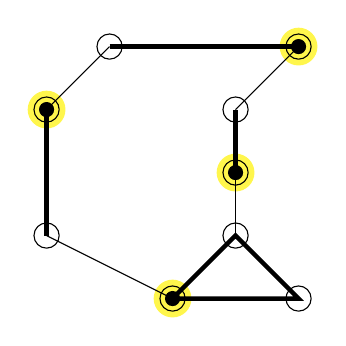
\begin{tikzpicture}[scale=0.8]
        \def\ver{0.12} %size of a vertex
        \def\xa{0}
        \def\ya{0}
        % Highlight change
        \draw[fill=yellow, opacity=.7, draw=none] (\xa-1,\ya-1)  circle (0.3cm);
        \draw[fill=yellow, opacity=.7, draw=none] (\xa-3,\ya+2) circle (0.3cm);
        \draw[fill=yellow, opacity=.7, draw=none] (\xa+1,\ya+3)  circle (0.3cm);
        \draw[fill=yellow, opacity=.7, draw=none] (\xa,\ya+1)  circle (0.3cm);

        %graph G
        \draw (\xa,\ya) circle (0.2cm);          % t11 no fill
        \draw (\xa+1,\ya-1) circle (0.2cm);      % t12 no fill
        \draw (\xa-1,\ya-1) circle (0.2cm);      % t13 no fill
        \draw (\xa-3,\ya) circle (0.2cm);        % e11 no fill
        \draw (\xa-3,\ya+2) circle (0.2cm);      % e12 no fill
        \draw (\xa-2,\ya+3) circle (0.2cm);      % e21 no fill
        \draw (\xa+1,\ya+3) circle (0.2cm);      % e22 no fill
        \draw (\xa,\ya+2) circle (0.2cm);        % e31 no fill
        \draw (\xa,\ya+1) circle (0.2cm);        % e32 no fill

        % Tokens
        \path[fill] (\xa-1,\ya-1) circle (\ver);   % t13
        \path[fill] (\xa-3,\ya+2) circle (\ver);   % e12
        \path[fill] (\xa+1,\ya+3) circle (\ver);   % e22
        \path[fill] (\xa,\ya+1) circle (\ver);     % e32

        % edges
        \draw[ultra thick] (\xa,\ya)--(\xa+1,\ya-1)--(\xa-1,\ya-1)--cycle;
        \draw[ultra thick] (\xa-3,\ya)--(\xa-3,\ya+2) ;
        \draw[ultra thick] (\xa-2,\ya+3)--(\xa+1,\ya+3) ;
        \draw[ultra thick] (\xa,\ya+2)--(\xa,\ya+1) ;

        \draw (\xa-2,\ya+3)--(\xa-3,\ya+2);
        \draw (\xa-3,\ya)--(\xa-1,\ya-1);
        \draw (\xa,\ya+1)--(\xa,\ya);
        \draw (\xa,\ya+2)--(\xa+1,\ya+3);

      \end{tikzpicture}
    \end{scaletikzpicturetowidth}
    \caption{An example of a restricted instance graph $G$ together with a standard token configuration.}
    \label{fig:standard_sliding}
\end{figure}


We say that a token configuration $T$ of $G_s$ is \textit{standard} if each token triangle and token edge of $G_s$ contains exactly one token
in $T$. Then, any move from a standard token configuration results in another standard token configuration since any token will never leave its
token triangle or token edge, and will never slide along a link edge because the first time any token would slide to another triangle or edge,
it would become adjacent to the token belonging to this triangle or edge. So tokens may never slide along a link edge. It is this latter
observation that will allow us to prove the $\PSPACE$-hardness of the labelled variant while doing only a little modification
in the original proof.

The sliding tokens problem remains $\PSPACE$-complete even if $G_s$ is such a restricted graph and both $T_0$ and $T_t$ are standard token
configurations \cite{bonsma}. This restricted problem is called the Standard sliding tokens problem.


\chapter{Reconfiguration of satisfiability problems} \label{chap:SAT}

In this chapter, boolean satisifiability reconfiguration problems are presented. For decades the Boolean satisfiability problem also known
as SAT has fascinated scientific world. In 1978 Schaefer proposed a framework for expressing variants of the satisfiability problem,
and showed a dichotomy theorem: the satisfiability problem for certain classes of Boolean formulas is in $\P$ while it is $\NP$-complete for
all other classes in the framework \cite{schaefer_complexity_1978}. In a single stroke, this result pinpoints the computational complexity
of all well-known variants of SAT, such as $3$-SAT, HORN $3$-SAT, NOT-ALL-EQUAL $3$-SAT, and 1-IN-$3$ SAT \cite{DBLP:journals/siamcomp/GopalanKMP09}.
Since then, dichotomies or trichotomies have been established for several aspects of the satisfiability problem such as optimization
\cite{CREIGNOU1995511,khanna_approximability_2001}, inverse satisfiability \cite{kavvadias_inverse_nodate}, minimal satisfiability \cite{KIROUSIS200320},
and 3-valued satisfiability \cite{10.1145/1120582.1120584}.


Continuing Schaefer's work, Gopalan et al. were interested by the connectivity properties of the solution graph motivated mainly by research
on satisfiability algorithms and the satisfiability threshold. The structure of the solution space of Boolean formulas can be characterized by
a $\textit{solution graph}$ where the vertices are the solutions (satisfying assignments) and two solutions are connection iff they differ in exactly
one variable. The connectivity problem (Conn) is to decide whether the solutions of a given Boolean formula $\varphi$ on $n$ variables induce a
connected subgraph of the $n$-dimensional hypercube, while the st-connectivity problem (st-Conn) is to decide whether two specific
solutions $s$ and $t$ of $\varphi$ are connected. Concerning the st-connectivity question, they proved dichtomies for the diameter of connected components
and the complexity. For the connectivity question, they conjectured a trichotomy. Building on this work, recently the trichotomy was
established by Schwerdtfeger in \cite{schwerdtfeger_computational_2015} and showed that Conn is either in $\P$, $\coNP$-complete, or $\PSPACE$-complete.


Recently, Gopalan et al.'s results have been applied to reconfiguration problems, mostly the st-connectivity and connectivity questions have been
applied to reconfiguration problems such as INDEPENDENT-SET RECONFIGURATION, GRAPH-k-COLORING RECONFIGURATION, and many complexity results were obtained.


\textit{Roadmap.} In section \ref{sec:schaefer's framework} we introduce Schaefer's framework and remarkable results, followed by section
\ref{sec:gopalan-et-al.'s-results} presenting Gopalan et al.'s results. Finally in section \ref{sec:a-computational-trichotomy} we present
Schwerdtfeger's results which establishes the trichotomy conjectured by Gopalan et al.'s for the connectivity problem.


% ----------------------------------------------------------------------------------------------------------------------------------
% ~~~~~~~~~~~~~~~~~~~~~~~~~~~~~~~~~~~~~~~~~~~~~~~~~~~~~~~~~~~~~~~~~~~~~~~~~~~~~~~~~~~~~~~~~~~~~~~~~~~~~~~~~~~~~~~~~~~~~~~~~~~~~~~~~~
% ----------------------------------------------------------------------------------------------------------------------------------
\section{Schaefer's framework}\label{sec:schaefer's framework}
Schaefer identified the complexity of every satisfiability problem SAT($\mathcal{S}$), where $\mathcal{S}$ ranges over all finite sets of
logical relations \cite{schwerdtfeger_computational_2015}. To state Schaefer’s main result, we need to define some basic concepts.
We will use the standard notions and definitions defined in \cite{schaefer_complexity_1978} and \cite{DBLP:journals/siamcomp/GopalanKMP09}.

\subsection{Preliminaries}

A CNF-formula is a Boolean formula of the form $C_{1} \land \dots \land C_{m}$, where each $C_i$ is a finite disjunction of literals where $C_i$
is referred to as a clause. A $k$-CNF formula $(k \geq 1)$ is a CNF-formula where each $C_i$ has at most $k$ literals.


A \textit{logical relation} $R$ is a non-empty subset of $\{0,1\}^n$, for some $n \geq 1$ where $n$ is the \textit{arity} of $R$.
A logical relation is a function that takes as input a Boolean vector and returns a Boolean. For a set $\mathcal{S}$ of logical relations, a
$\mathcal{S}$-formula is a conjuntion of logical relations from $\mathcal{S}$, where the arguments of each relation are freely chosen among
a set of variables.

For a finite set of relations $\mathcal{S}$, a $CNF(\mathcal{S})$-formula over a set of variables $V = \{x_1, \dots, x_n\}$ is a finite
conjunction $C_{1} \land \dots \land C_{m}$, where each $C_i$ is an expression of the form $R(\xi_1,\dots , \xi_k)$, with a $k$-ary
relation $R \in S$, and each $\xi_j$ is a variable from $V$ or one of the constants $0, 1$. A $\textit{solution}$ if a
CNF($\mathcal{S}$)-formula $\varphi$ is an assignment $s = (a_{1}, \dots, a_{n})$ of Boolean values to the variables that makes every
clause of $\varphi$ true. A CNF($\mathcal{S}$)-formula is $\textit{satisfiable}$ if it has at least one solution.

The satisfiability problem SAT($\mathcal{S}$) associated with a finite set $\mathcal{S}$ of logical relations asks:
given a CNF($\mathcal{S}$)-formula $\varphi$, is it satisfiable? All well known restrictions of Boolean satisfiability, such as $3$-SAT,
NOT-ALL-EQUAL $3$-SAT, and POSITIVE $1$-IN-$3$ SAT, can be cast as SAT$(\mathcal{S})$ problems, for a suitable choice of $\mathcal{S}$.

Schaefer identified the complexity of every satisfiability problem SAT($\mathcal{S}$), where $\mathcal{S}$ ranges over all finite sets of
logical relations. To state Schaefer’s main result, we need to define some properties and relations for $R$ and $\mathcal{S}$.

\begin{defn} Let $R$ be a logical relation.
    \begin{enumerate}
        \item $R$ is \textit{bijunctive} if it is the set of solutions of a $2$-CNF formula.
        \item $R$ is \textit{Horn} if it is the set of solutions of a Horn formula, where a Horn formula is a CNF-formula where each $C_i$ has at most
        one positive literal.
        \item $R$ is \textit{dual Horn} if it is the set of solutions of a dual Horn formula, where a dual Horn formula is a CNF-formula where each
        $C_i$ has at most one negative literal.
        \item $R$ is \textit{affine} if it is the set of solutions of a system of linear equations over $\mathcal{Z}_2$.
    \end{enumerate}
\end{defn}

\begin{defn}A set $S$ of logical relations is Schaefer if at least one of the following conditions holds:
    \begin{enumerate}
        \item Every relation in $\mathcal{S}$ is bijunctive.
        \item Every relation in $\mathcal{S}$ is Horn.
        \item Every relation in $\mathcal{S}$ is dual Horn.
        \item Every relation in $\mathcal{S}$ is affine.
    \end{enumerate}
\end{defn}

We are now ready to present Schaefer's theorem :
\begin{theorem}{(Schaefer’s Dichotomy Theorem \cite{schaefer_complexity_1978})} Let $S$ be a finite set of logical relations. If $\mathcal{S}$ is Schaefer, then
SAT($\mathcal{S}$) is in $\P$; otherwise, SAT($\mathcal{S}$) is $\NP$-complete.
\end{theorem}\label{theorem:dichotomy}

Theorem \ref{theorem:dichotomy} is called a dichotomy theorem because Ladner \cite{ladner} has shown that if $\P \neq \NP$, then there are problems
in $\NP$ that are neither in $\P$, nor $\NP$-complete. Thus, Theorem \ref{theorem:dichotomy} asserts that no SAT($\mathcal{S}$) problem
is a problem of the kind discovered by Ladner.



% ----------------------------------------------------------------------------------------------------------------------------------
% ~~~~~~~~~~~~~~~~~~~~~~~~~~~~~~~~~~~~~~~~~~~~~~~~~~~~~~~~~~~~~~~~~~~~~~~~~~~~~~~~~~~~~~~~~~~~~~~~~~~~~~~~~~~~~~~~~~~~~~~~~~~~~~~~~~
% ----------------------------------------------------------------------------------------------------------------------------------
\section{Gopalan et al.'s results}\label{sec:gopalan-et-al.'s-results}

Gopalan et al. continued expanding Schaefer's dichotomie and focused on the connectivity of Boolean satisfiability. They believed
that the connectivity properties of Boolean satisfiability merit some study in their own right, as they shed light on the structure of the solution
space of Boolean formulas thus specifically addressed CNF($\mathcal{S}$)-formulas and studied the complexity of the
following two decision problems,
\begin{itemize}
    \item the connectivity problem $Conn(S)$, that asks for a given $CNF(S)$-formula $\varphi$ whether $G(\varphi)$ is connected,
    \item the st-connectivity problem $st-Conn(S)$, that asks for a given $CNF(S)$-formula $\varphi$ and two solutions $s$ and $t$ whether
    there a path from $s$ to $t$ in $G(\varphi)$.
\end{itemize}

\subsection{Complexity-theoric dichotomies}
Schaefer showed that the satisfiability problem is solvable in polynomial time precisely for formulas built from Boolean
relations all of which are bijunctive, or all of which are Horn, or all of which are dual Horn, or all of which are affine. Gopalan et al.
identified new classes of Boolean relations, called \textit{tight relations}, that properly contain the classes of bijunctive, Horn, dual Horn,
and affine relations. They then showed that st-connectivity is solvable in linear time for formulas built from tight relations,
and $\PSPACE$-complete in all other cases. Their second main result is a dichotomy theorem for the connectivity
problem: it is in $\coNP$ for formulas built from tight relations, and $\PSPACE$-complete in all other cases.

\subsection{Structural dichotomy theorem}
In addition to these two complexity-theoretic dichotomies, they established a structural dichotomy theorem for the diameter of the connected
components of the solution space of Boolean formulas. This result asserts that, in the $\PSPACE$-complete cases, the diameter of
the connected components can be exponential, but in all other cases it is linear. Thus, small
diameter and tractability of the st-connectivity problem are remarkably aligned.

Their results are summarized in comparison to the satisfiability problem SAT($\mathcal{S})$ in table \ref{tab:1}.
\begin{table}[h!]
    \centering
    \begin{tabular}{|c || c | c | c | c |}
        \hline
        $\mathcal{S}$ & SAT($\mathcal{S}$) & ST-CONN($\mathcal{S}$) & CONN($\mathcal{S}$) & Diameter \\ [0.5ex]
        \hline\hline
        Schaefer & $\P$ & $\P$ & $\coNP$ & $O(n)$ \\
        Tight, not Schaefer & $\NP$-compl. & $\P$ & $\coNP$-compl. & $O(n)$ \\
        Not tight & $\NP$-compl. & $\PSPACE$-compl. & $\PSPACE$-compl. & $2^{\Omega (\sqrt{n}) }$ \\ [1ex]
        \hline
    \end{tabular}
    \caption{Gopalan et al.’s results \cite{gopalan_connectivity_2006}}
    \label{tab:1}
\end{table}


\section{A computational Trichotomy for Conn(S)}\label{sec:a-computational-trichotomy}
Schwerdtfeger investigated issues in Gopalan et al.'s work and argued that repeated occurrences of variables in constraint applications
can make the problems harder and the diameter exponential in some cases. This lead to a slight shift of the boundaries established by
Gopalan et al.'s in the hard direction and an introduction to the new classes called \textit{safely tight} and relations \textit{CPSS} fitted to
the correct boundaries.


The following table summarizes their results.
\begin{table}[h!]
    \centering
    \begin{tabular}{|c || c | c | c | c |}
        \hline
        $\mathcal{S}$ & SAT($\mathcal{S}$) & ST-CONN($\mathcal{S}$) & CONN($\mathcal{S}$) & Diameter \\ [0.5ex]
        \hline\hline
        CPSS & $\P$ & $\P$ & $\P$ & $O(n)$ \\
        Schaefer, not CPSS & $\P$ & $\P$ & $\coNP$-compl. & $O(n)$ \\
        Safely tight, not Schaefer & $\NP$-compl. & $\P$ & $\coNP$-compl. & $2^{\Omega (\sqrt{n}) }$ \\
        Not safely tight & $\NP$-compl. & $\PSPACE$-compl. & $\PSPACE$-compl. & $2^{\Omega (\sqrt{n}) }$ \\ [1ex]
        \hline
    \end{tabular}
    \caption{Complete classification of the connectivity problems and the diameter
    for CNF($\mathcal{S}$)-formulas with constants, in comparison to SAT \cite{schwerdtfeger_computational_2015}}
    \label{tab:2}
\end{table}



\chapter{Subset sum Reconfiguration}
The subset sum problem is a well-known \NP-complete problem in which given an integer $x$ and a set of integers $S = \{a_1, a_2,\dots, a_n\}$,
we wish to find a subset $A \subseteq [n]$ such that $\sum_{i \in A} a_{i} = x$.

In \cite{Ito11approximabilityof}, Ito and Demaine considered the following problem :
Given two \textit{packings}\footnote{Please refer to \cite{Ito11approximabilityof} for the definition of packings} $A_1$ and $A_2$, both of total
size at least $k$, can we transform $A_1$ into $A_2$ via packings by moving (namely, either adding or removing) a
single item to/from the previous one without ever going through a packing of total size less than $k$. This problem is referred to as the
SUBSET SUM RECONFIGURATION problem and is proved to be strongly $\NP$-hard, and $\PSPACE$-complete for the variant with conflict graph
\cite{Ito11approximabilityof}.

In this chapter, we explore another reconfiguration version of the subset sum problem referred to as the $k$-move Subset Sum reconfiguration
problem presented in \cite{cardinal_reconfiguration_2018}. We say that a set of integers $A_1$ can be \textit{$k$-move reconfigured} into a
second set of integers $A_2$ whenever the symmetric difference of $A_1$ and $A_2$ has cardinality at most $k$. It turns out that the
$k$-move Subset Sum reconfiguration problem is $\PSPACE$-complete \cite{cardinal_reconfiguration_2018}. This chapter is dedicated to this
result. 

\textit{Roadmap.} This chapter is organised in the following way : Sections \ref{sec:k_move_sec} to \ref{sec:Exact_cover} introduces
the $k$-move subset sum reconfiguration problem, the labelled sliding token problem and the exact cover problem reconfiguration problem
respectively along with proofs of their complexity results added with illustrative examples to help visualize the concepts.

\section{$k$-move Subset Sum Reconfiguration}\label{sec:k_move_sec}
To begin our journey to the hardness proof of the $3$-move subset sum reconfiguration problem, we first start by defining the decision
problem of the $k$-move subset sum reconfiguration.
\begin{defn}{($k$-move Subset Sum Reconfiguration Problem).} Given two solutions $A_1$ and $A_2$ to an instance of the subset sum problem,
can $A_2$ be obtained by repeated $k$-move reconfiguration, beginning with $A_1$, so that all intermediate subsets are also solutions?
\end{defn}

Notice that the reconfiguration problem is trivial if the reconfiguration steps are restricted to involve only the removal or addition of a single element
of $S$, as no single such move can maintain the same sum. The problem remains trivial for $k=2$, since any removed element must be replaced by
itself. For $k=3$, the following theorem is proved:
\begin{theorem}The $3$-move Subset Sum Reconfiguration problem is strongly $\PSPACE$-complete.\end{theorem} \label{theorem:3_move}


The proof of theorem \ref{theorem:3_move} is organised in the following way : We first start by proving the membership of the $k$-move subset
sum reconfiguration problem in $\PSPACE$ (lemma \ref{lemma:k_move_pspace}). Proving the hardness is done in two steps. The first step
consists of reducing the labelled Sliding Token Reconfiguration problem to the Exact Cover Reconfiguration problem (lemma \ref{lemma:ECR}).
However before diving into the proof of lemma \ref{lemma:ECR}, we first take a detour to sections \ref{sec:sliding_problem} and
\ref{sec:Exact_cover} where the labelled sliding token reconfiguration and exact cover reconfiguration problems are introduced respectively.

The second step involves reducing the Exact Cover Reconfiguration problem to the $3$-move Subset Sum Reconfiguration problem
(theorem \ref{theorem:3_move_theorem}).

\begin{lemma}For every $k \in \mathbb{N}$, the $k$-move Subset Sum Reconfiguration problem is in $\PSPACE$. \end{lemma} \label{lemma:k_move_pspace}
\begin{proof}
For an instance with $|S| = n$, there are $O(n^{k})$ other subsets reachable by a $k-$move reconfiguration, since each such move can be specified
by the set of items in the symmetric difference of the two subsets. So all adjacent subsets in the reconfiguration graph can be enumerated in
polynomial time. Then the $k$-move subset sum reconfiguration problem is in $\NPSPACE$ by the following algorithm : in the reconfiguration graph,
repeatedly move between subsets by  non-deterministically selecting a neighbour in polynomial time and space. Since \NPSPACE $=$ \PSPACE
\cite{savitch_relationships_1970}, the $k$-move subset sum is also in $\PSPACE$.
\end{proof}

\section{Labelled SLIDING TOKEN problem.}\label{sec:sliding_problem}
The Sliding token problem is introduced in chapter \ref{chap:NCL} and detailed in section \ref{sec:sliding_tokens}. Hearn and Demaine proved that
the SLIDING TOKEN PROBLEM is $\PSPACE$-complete for planar graphs \cite{hearn_pspace-completeness_2004}, as an example of the application of
the nondeterministic constraint logic model and they implicitly proved that the SLIDING TOKEN PROBLEM is $\PSPACE$-hard on $3$-regular graphs
since the reduction is done from a restricted NCL machine (NCL-CONFIGURATION-TO-EDGE) in which the underlying graph is planar and all vertices
have degree three. The labelled variant of the sliding token problem, where each token has a unique label, is also $\PSPACE$-hard and is proved
in section \ref{sec:labelled_sliding_token} of chapter \ref{chap:NCL}.

\section{Exact Cover Reconfiguration problem} \label{sec:Exact_cover}
The exact cover reconfiguration problem is the second problem introduced along this reduction. It will be referred to as the
ECR problem throughout the rest of this thesis. The variant of the ECR problem considered here is the Exact cover split and merge
reconfiguration defined as follows :

\begin{defn}{(Exact Cover Split and Merge Reconfiguration).} Given a set $\mathcal{S}$ of subsets of a set $\mathcal{U}$, and two exact covers
$C_1$ and $C_2 \subseteq \mathcal{S}, C_1$ can be reconfigured into $C_2$ via a split (and $C_2$ can be reconfigured into $C_1$ via a merge)
provided that there exist $S_1, S_2, S_3 \subseteq \mathcal{S}$ with $C_1 - C_2 = S_1$ and $C_2 - C_1 = \{s_2, s_3\}$.

Since $C_1, C_2$ are exact covers it is mandatory that $S_1 = S_2 \cup S_3$ and $ S_2 \cap S_3 = \emptyset$.
\end{defn}

Thus, the ECR decision problem can be reformulated as follows :
\begin{defn}{(Exact Cover Reconfiguration problem).} Given a set $\mathcal{S}$ of subsets of a set $\mathcal{U}$, and two configuration
$C_1$ and $C_2$, can $C_1$ be reconfigured into $C_2$ via repeated splits and merges ?
\end{defn}

\begin{example}
Let $\mathcal{U} = \{1,2,3\}$ and $\mathcal{S} = \{\{1\}, \{2\}, \{3\}, \{1,2\}, \{2,3\}\}$ and the two given configurations be the
following : $C_1 = \{\{1\}, \{2,3\}\}$ and $C_2 = \{\{1,2\}, \{3\}\}$. A solution would be the following :

\begin{figure}[H]
\begin{center}
\begin{scaletikzpicturetowidth}{\textwidth}
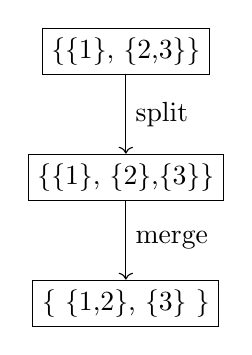
\begin{tikzpicture}[scale=1]
  \node (1) [draw, rectangle] {\{\{1\}, \{2,3\}\}};
  \node (2) [below=of 1, draw, rectangle] {\{\{1\}, \{2\},\{3\}\}};
  \node (3) [below=of 2, draw, rectangle] {\{ \{1,2\}, \{3\} \}};
  \draw[->]  (1) to node [auto] {split} (2);
  \draw[->]  (2) to node [auto] {merge} (3);
\end{tikzpicture}
\end{scaletikzpicturetowidth}
\end{center}
\caption{Reconfiguration sequence which transforms $C_1$ into $C_2$ via splits and merges.}\label{fig:exact_cover}
\end{figure}
\end{example}

\subsection{$k$-colourability}
Recall that a set $\mathcal{S}$ of subsets of a set $U$ can be considered as a hypergraph $H = (U, \mathcal{S})$, where each element
of $U$ is a vertex and each element of $\mathcal{S}$ is a hyperedge. We say that a hypergraph is $k$-colourable whenever we
can assign one of $k$ colours to each vertex such that no two vertices in a hyperedge have the same colour. The colourability of the ECR
problem is introduced for further use.

\subsection{$\PSPACE$-hardness result of the ECR problem.} \label{subsection:ECR_problem}
In this section we prove the hardness result of the ECR problem as the first step in order to prove theorem \ref{theorem:3_move}. This is done
by reducing the labelled variant of the SLIDING TOKEN PROBLEM to the Exact Cover Reconfiguration problem as mentioned earlier.

The proof is structured in the following way : First the input instance of the labelled sliding token reconfiguration problem is presented in
section \ref{subsubsection:input_instance}, followed by the definition of some terms used in the reduction proof in section 
\ref{subsubsection:prelim}. The output instance is described in section \ref{subsubsection:output_instance}.
Sections \ref{subsubsection:high_level} to \ref{subsubsection:23_colorability} are devoted to the proof.

\begin{lemma}The Exact Cover Reconfiguration problem is $\PSPACE$-hard for instances that are $23$-colourable hypergraphs. \end{lemma} \label{lemma:ECR}
\begin{proof}labelled variant of the SLIDING TOKEN PROBLEM $\leq_p$ Exact Cover Reconfiguration problem.

\subsubsection{Input instance of the labelled SLIDING TOKEN PROBLEM}\label{subsubsection:input_instance}
\begin{itemize}
  \item $G = (V,E)$, a $3$-regular graph.
  \item $T$, a set of labelled tokens.
  \item $p_1 : T \rightarrow V,$ a function mapping each labelled token to a vertex placement in the starting configuration of the output instance.
  \item $p_2 : T \rightarrow V,$ a function mapping each labelled token to a vertex placement in the ending configuration of the output instance.
  \item $I_1 = \{p_1(t) : t \in T\}$ and $I_2 = \{p_2(t) : t \in T\}$ are independent sets of size $|T| \leq |V|$.
\end{itemize}

\begin{example}{Input instance of the labelled SLIDING TOKEN PROBLEM}
  \begin{figure}[H]
    \centering
    \begin{subfigure}[b]{0.4\textwidth}
      \begin{scaletikzpicturetowidth}{\textwidth}
        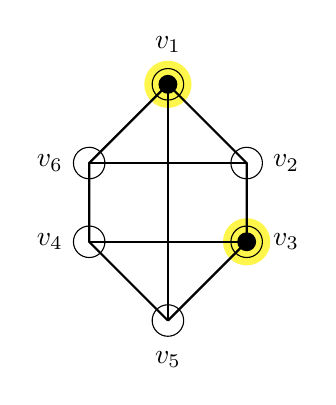
\begin{tikzpicture}[scale=1]
          \def\ver{0.12} %size of a vertex
          \def\xa{0}
          \def\ya{0}
          % Highlight change
          \draw[fill=yellow, opacity=.7, draw=none] (\xa,\ya+3)  circle (0.3cm); % v1
          \draw[fill=yellow, opacity=.7, draw=none] (\xa+1,\ya+1) circle (0.3cm);  % v3
          % graph G
          \draw (\xa,\ya) circle (0.2cm);          % v5
          \draw (\xa+1,\ya+1) circle (0.2cm);      % v3
          \draw (\xa+1,\ya+2) circle (0.2cm);      % v2
          \draw (\xa,\ya+3) circle (0.2cm);        % v1
          \draw (\xa-1,\ya+2) circle (0.2cm);      % v6
          \draw (\xa-1,\ya+1)circle (0.2cm);       % v4
          % Tokens
          \path[fill] (\xa,\ya+3) circle (\ver);   % v1
          \path[fill] (\xa+1,\ya+1) circle (\ver); % v3
          % labels
          \node (1) at (\xa,\ya+3.5) {$v_1$};     % v1
          \node (2) at (\xa+1.5,\ya+2) {$v_2$};   % v2
          \node (3) at (\xa+1.5,\ya+1) {$v_3$};   % v3
          \node (5) at (\xa,\ya-0.5) {$v_5$};     % v5
          \node (4) at (\xa-1.5,\ya+1) {$v_4$};   % v4
          \node (6) at (\xa-1.5,\ya+2) {$v_6$};   % v6
          %edges
          \draw[thick] (\xa,\ya)--(\xa+1,\ya+1)--(\xa+1,\ya+2)--(\xa,\ya+3)--(\xa-1,\ya+2)--(\xa-1,\ya+1)--(\xa,\ya) ; % contour
          \draw[thick] (\xa,\ya)--(\xa,\ya+3) ;       % v5 - v1
          \draw[thick] (\xa+1,\ya+1)--(\xa-1,\ya+1) ; % v3 - v4
          \draw[thick] (\xa+1,\ya+2)--(\xa-1,\ya+2) ; % v2 - v6
        \end{tikzpicture}
      \end{scaletikzpicturetowidth}
      \caption{Initial configuration $S_{1}$.}
      \label{fig:standard_1}
    \end{subfigure}
    \begin{subfigure}[b]{0.4\textwidth}
      \begin{scaletikzpicturetowidth}{\textwidth}
        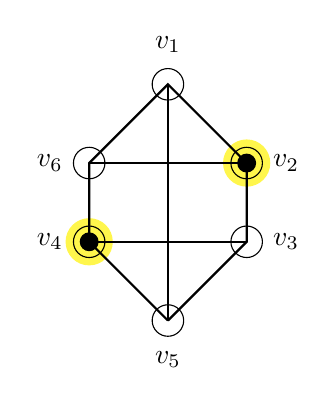
\begin{tikzpicture}[scale=1]
          \def\ver{0.12} %size of a vertex
          \def\xa{0}
          \def\ya{0}
          % Highlight change
          \draw[fill=yellow, opacity=.7, draw=none] (\xa+1,\ya+2)  circle (0.3cm); % v2
          \draw[fill=yellow, opacity=.7, draw=none] (\xa-1,\ya+1) circle (0.3cm);  % v4
          % graph G
          \draw (\xa,\ya) circle (0.2cm);          % v5
          \draw (\xa+1,\ya+1) circle (0.2cm);      % v3
          \draw (\xa+1,\ya+2) circle (0.2cm);      % v2
          \draw (\xa,\ya+3) circle (0.2cm);        % v1
          \draw (\xa-1,\ya+2) circle (0.2cm);      % v6
          \draw (\xa-1,\ya+1) circle (0.2cm);      % v4
          % Tokens
          \path[fill] (\xa+1,\ya+2) circle (\ver);   % v2
          \path[fill] (\xa-1,\ya+1) circle (\ver);   % v4
          % labels
          \node (1) at (\xa,\ya+3.5) {$v_1$};     % v1
          \node (2) at (\xa+1.5,\ya+2) {$v_2$};   % v2
          \node (3) at (\xa+1.5,\ya+1) {$v_3$};   % v3
          \node (5) at (\xa,\ya-0.5) {$v_5$};     % v5
          \node (4) at (\xa-1.5,\ya+1) {$v_4$};   % v4
          \node (6) at (\xa-1.5,\ya+2) {$v_6$};   % v6
          %edges
          \draw[thick] (\xa,\ya)--(\xa+1,\ya+1)--(\xa+1,\ya+2)--(\xa,\ya+3)--(\xa-1,\ya+2)--(\xa-1,\ya+1)--(\xa,\ya) ; % contour
          \draw[thick] (\xa,\ya)--(\xa,\ya+3) ;       % v5 - v1
          \draw[thick] (\xa+1,\ya+1)--(\xa-1,\ya+1) ; % v3 - v4
          \draw[thick] (\xa+1,\ya+2)--(\xa-1,\ya+2) ; % v2 - v6
        \end{tikzpicture}
      \end{scaletikzpicturetowidth}
      \caption{Target configuration $S_{2}$.}
      \label{fig:standard_2}
    \end{subfigure}
    \caption{A Standard sliding token instance with initial and target labelled token configuration $S_{1}$ and $S_{2}$ respectively with a
    set of labelled tokens $T = \{t_1, t_2\}$ and $p_{1}(T_{A}) = \{v_1, v_3\}$ and $p_{2}(T_{B}) = \{v_2, v_4\}$ (the mapping is shown by
    the highlighted vertices).}
    \label{fig:input_instance_standard}
  \end{figure}
\end{example}

\subsubsection{Preliminaries} \label{subsubsection:prelim}
Before diving in the proof resulr, a few notions that will be used are presented hereunder :
\paragraph{Slide Set.}
For each pair of adjacent vertices $v_i, v_j \in V$ of the input instance of the sliding token problem, the set consisting of these two vertices
and their neighbors is called a $slide set$, denoted $S_{i,j}$.
\begin{figure}[H]
  \begin{center}
    \begin{scaletikzpicturetowidth}{\textwidth}
      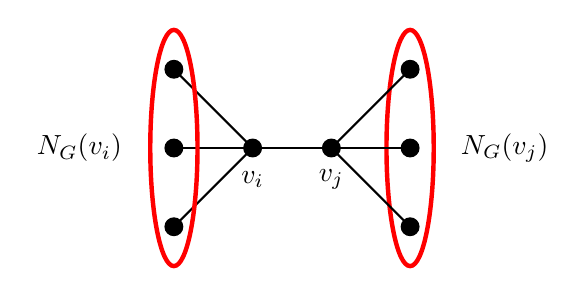
\begin{tikzpicture}[scale=1]
      \def\ver{0.12} %size of a vertex
      \def\x{1}
      \def\xa{1}
      \def\ya{0}
      \def\xb{2}
      %Slide Set
      \path[fill] (\xa,\ya) circle (\ver);       % vi
      \node (1) at (\xa,\ya-0.4) {$v_i$};
      \path[fill] (\xa-1,\ya) circle (\ver);     % v2
      \path[fill] (\xa-1,\ya+1) circle (\ver);   % v1
      \path[fill] (\xa-1,\ya-1) circle (\ver);   % v3

      \draw[thick] (\xa,\ya)--(\xa-1,\ya) ;
      \draw[thick] (\xa,\ya)--(\xa-1,\ya+1) ;
      \draw[thick] (\xa,\ya)--(\xa-1,\ya-1) ;
      \draw[ultra thick, red] (0,0) ellipse (0.3 and 1.5);
      \node (3) at (\xa-2.2,\ya) {$N_{G}(v_i)$};
      \draw[ultra thick, red] (3,0) ellipse (0.3 and 1.5);
      \node (3) at (\xb+2.2,\ya) {$N_{G}(v_j)$};

      %graph independent set
      \path[fill] (\xb,\ya) circle (\ver);       % v_j
      \node (1) at (\xb,\ya-0.4) {$v_j$};
      \path[fill] (\xb+1,\ya) circle (\ver);    % v2
      \path[fill] (\xb+1,\ya+1) circle (\ver);   % v1
      \path[fill] (\xb+1,\ya-1) circle (\ver);   % v3
      \draw[thick] (\xb,\ya)--(\xb+1,\ya) ;
      \draw[thick] (\xb,\ya)--(\xb+1,\ya+1) ;
      \draw[thick] (\xb,\ya)--(\xb+1,\ya-1) ;

      \draw[thick] (\xa,\ya)--(\xb,\ya) ;
      \end{tikzpicture}
    \end{scaletikzpicturetowidth}
  \end{center}
  \caption{Slide set denoted $S_{ij}$ of vertices $v_i$ and $v_j$.}
  \label{fig:slide_set}
\end{figure}

\paragraph{Maximally split configuration $C$.}
A configuration $C$ of the output Exact Cover instance is called \textit{maximally split} if every $c \in C$
contains exactly one vertex and up to one token.

\begin{example}{A maximally split configuration $C$}
  \begin{figure}[h!]
    \begin{center}
      \begin{scaletikzpicturetowidth}{\textwidth}
        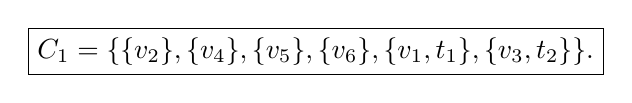
\begin{tikzpicture}[scale=1]
          \node (1) [draw, rectangle] {$C_1 = \{ \{v_2\}, \{v_4\}, \{v_5\}, \{v_6\}, \{v_1, t_1\}, \{v_3, t_2\} \}$.};
        \end{tikzpicture}
      \end{scaletikzpicturetowidth}
    \end{center}
    \caption{A maximally split configuration $C_1$.}
    \label{}
  \end{figure}
\end{example}

\paragraph{Sploot set of a configuration $C$.}
For each exact cover configuration $C$ in the output instance, let sploot($C$) be the set of all maximally split configurations reachable from $C$.


\subsubsection{Output $\mathcal{U}$ and $\mathcal{S}$}\label{subsubsection:output_instance}
The output instance of the Exact Cover Reconfiguration problem contains a set $\mathcal{S}$ of subsets of a set $\mathcal{U}$ defined in
\ref{sec:Exact_cover} where :
\begin{itemize}
  \item $\mathcal{U} = \{v_1, v_2, \dots, v_{|V|}\} \cup \{t_1, t_2, \dots, t_{|T|}\}.$
  \item The set $\mathcal{S}$ is defined as follows, for every pair of adjacent vertices $v_i, v_j$ and token $t_k$
    \begin{itemize}
      \item All subsets of $S_{i,j} - \{v_i\}$ and $S_{i,j} - \{v_j\}$.
      \item $\{v_i, t_k\}$ and $\{v_j , t_k\}$.
      \item $S_{i,j} \cup \{t_k\}$.
    \end{itemize}
\end{itemize}

\begin{example}According to the above example, \ref{fig:input_sliding_token_example}, the output instance of the Exact Cover Reconfiguration
problem is the following : \todo{Do the output instance in tikz}
\end{example}

\subsubsection{Output exact cover starting and ending configurations, $C_1$ and $C_2$}
The starting configuration $C_1$ is the union of $\{\{ v_i \} : v_i \in V - I_1\}$ and, for every $v_i \in I_1$, a set $\{v_i, t_k\}$ with a
distinct $t_k$.
The ending configuration $C_2$ is then the union of $\{\{ v_i \} : v_i \in V - I_2\}$ and, for every $v_i \in I_2$, a set $\{v_i, t_k\}$ with a
distinct $t_k$.

\begin{example}Continuing the running example, $C_1$ and $C_2$ would be :
\begin{itemize}
  \item $C_1 = \{ \{v_2, v_4, v_5, v_6\}, \{v_1, t_1\}, \{v_3, t_2\}\}$.
  \item $C_2 = \{ \{v_1, v_3, v_5, v_6\}, \{v_2, t_1\}, \{v_4, t_2\}\}$.
\end{itemize}
\end{example}

\subsubsection{$23$-colourability of the output instance $H = (U, \mathcal{S})$}\label{subsubsection:23_colorability}
The goal here is to make sure that no two vertices of distance at most $3$ (i.e. in a common slide set see figure \ref{fig:slide_set}) have the same
colour. More precisely, we want to prove that given $23$-colours, no two vertices having a common slide set would have the same colour.
This constraint will enforce the absence of tokens on neighbors of $v_i$ and $v_j$, and the presence of a token on $v_i$ or $v_j$, but not both
making sure that any merge or split will result into a feasible configuration.

Given that the $kth$ power $G^{k}$ of an undirected graph $G$ is another graph that has the same set of vertices, but in which two vertices are
adjacent when their distance in $G$ is at most $k$, to find the colourability of the output instance $H = (U, \mathcal{S})$, it suffices to
compute $\Delta(G^{3})$. Since $G$ is $3-$regular, $G^3$ has degree at most $21$ proven by the following figure where the worst case
scenario.

\begin{figure} [H]
  \centering
  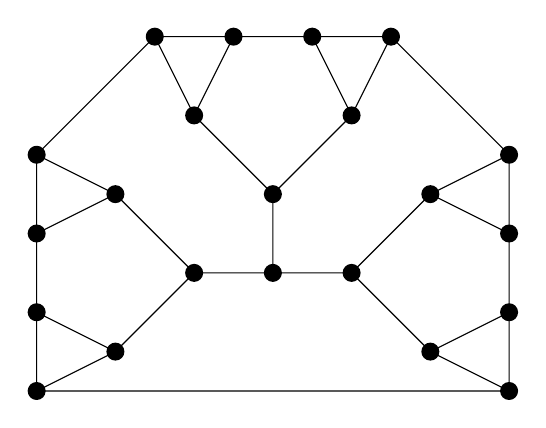
\begin{tikzpicture}
    \def\xa{0}
    \def\ya{0}
    %nodes
    \draw[thick, fill=black] (\xa,\ya) circle (0.1cm);           % v1

    \draw[thick, fill=black] (\xa+1,\ya) circle (0.1cm);         % v2
    \draw[thick, fill=black] (\xa+2,\ya+1) circle (0.1cm);       % v3
    \draw[thick, fill=black] (\xa+2,\ya-1) circle (0.1cm);       % v4
    \draw[thick, fill=black] (\xa+3,\ya-0.5) circle (0.1cm);     % v5
    \draw[thick, fill=black] (\xa+3,\ya-1.5) circle (0.1cm);     % v6
    \draw[thick, fill=black] (\xa+3,\ya+1.5) circle (0.1cm);     % v7
    \draw[thick, fill=black] (\xa+3,\ya+0.5) circle (0.1cm);     % v8

    \draw[thick, fill=black] (\xa,\ya+1) circle (0.1cm);         % v9
    \draw[thick, fill=black] (\xa+1,\ya+2) circle (0.1cm);       % v10
    \draw[thick, fill=black] (\xa-1,\ya+2) circle (0.1cm);       % v11
    \draw[thick, fill=black] (\xa+1.5,\ya+3) circle (0.1cm);     % v12
    \draw[thick, fill=black] (\xa+0.5,\ya+3) circle (0.1cm);     % v13
    \draw[thick, fill=black] (\xa-0.5,\ya+3) circle (0.1cm);     % v14
    \draw[thick, fill=black] (\xa-1.5,\ya+3) circle (0.1cm);     % v15

    \draw[thick, fill=black] (\xa-1,\ya) circle (0.1cm);         % v16
    \draw[thick, fill=black] (\xa-2,\ya+1) circle (0.1cm);       % v17
    \draw[thick, fill=black] (\xa-2,\ya-1) circle (0.1cm);       % v18
    \draw[thick, fill=black] (\xa-3,\ya-1.5) circle (0.1cm);     % v19
    \draw[thick, fill=black] (\xa-3,\ya-0.5) circle (0.1cm);     % v20
    \draw[thick, fill=black] (\xa-3,\ya+0.5) circle (0.1cm);     % v21
    \draw[thick, fill=black] (\xa-3,\ya+1.5) circle (0.1cm);     % v22

    %edges
    \draw (\xa,\ya)--(\xa+1,\ya)--(\xa+2,\ya-1)--(\xa+3,\ya-1.5) ;         % v1 - v2 - v4 - v6
    \draw (\xa+1,\ya)--(\xa+2,\ya+1)--(\xa+3,\ya+1.5) ;                      % v2 - v3 - v7
    \draw (\xa,\ya)--(\xa,\ya+1)--(\xa+1,\ya+2)--(\xa+1.5,\ya+3) ;     % v1 - v9 - v10 - v12
    \draw (\xa,\ya+1)--(\xa-1,\ya+2)--(\xa-1.5,\ya+3) ;            % v9 - v11 - v15
    \draw (\xa,\ya)--(\xa-1,\ya)--(\xa-2,\ya-1)--(\xa-3,\ya-1.5) ;   % v1 - v16 - v18 - v19
    \draw (\xa-1,\ya)--(\xa-2,\ya+1)--(\xa-3,\ya+1.5) ; % v16 - v17 - v22
    \draw (\xa-2,\ya-1)--(\xa-3,\ya-0.5) ; % v18 - v20
    \draw (\xa-2,\ya+1)--(\xa-3,\ya+0.5) ; % v17 - v21
    \draw (\xa-1,\ya+2)--(\xa-0.5,\ya+3) ; % v11 - v14
    \draw (\xa+1,\ya+2)--(\xa+0.5,\ya+3) ; % v10 - v13
    \draw (\xa+2,\ya+1)--(\xa+3,\ya+0.5) ;  % v3 - v8
    \draw (\xa+2,\ya-1)--(\xa+3,\ya-0.5) ; % v4 - v5

    \draw (\xa+3,\ya-1.5)--(\xa-3,\ya-1.5)--(\xa-3,\ya-0.5)--(\xa-3,\ya+0.5)--(\xa-3,\ya+1.5)--(\xa-1.5,\ya+3)--(\xa-0.5,\ya+3)--(\xa+0.5,\ya+3)--(\xa+1.5,\ya+3)--(\xa+3,\ya+1.5)--(\xa+3,\ya+0.5)--(\xa+3,\ya-0.5)--(\xa+3,\ya-1.5)--(\xa-3,\ya-1.5) ; %contour

  \end{tikzpicture}
  \caption{Graph $G^{'}$ (shown darker) is a subgraph of $G$.}
  \label{fig:subgraph}
\end{figure}


So $G$ can be $22-$coloured such that no two vertices of distance at most $3$ have the same colour. Colouring the tokens in $\mathcal{T}$
a distinct (23rd) colour then gives a colouring of $\mathcal{U}$ such that no pair of elements of a common set share the same colour.

\subsubsection{High level idea}\label{subsubsection:high_level}
We first note that the subsets containing exactly one vertex and a token (e.g., $\{v_i, t_k\}$) represents the presence of the token
$t_k$ on vertex $v_i$ and the subsets consisting of a slide set and a token (e.g., $\{S_{i,j} \cup t_k\}$) represent the presence of a
"mid-slide" token between $v_i$ and $v_j$. A "mid-slide" token can be interpreted as the token $t_k$ not being properly on $v_i$ or $v_j$ but is
"on it's way" from $v_i$ to $v_j$. Therefore, sliding a token $t_k$ from $v_i$ to $v_j$ is simulated by first
merging $\{v_i, t_k\}$ and $S_{i,j}-\{v_i\}$ into $S_{i,j} \cup \{t_k\}$, and then splitting this set into this set into $S_{i,j}-\{v_j\}$
and ${v_j, t_k}$. The first step of this sequence enforces the absence of tokens on neighbors of $v_i$ and $v_j$ since by definition, the slide
set $S_{ij}$ of $v_i$ and $v_j$ contains all the of $v_i$ and $v_j$ and having the token $t_k$  merged in $S_{ij}$ means that $t_k$ is not on any
vertex. The second step then ensures the presence of a token on $v_i$ or $v_j$, but not both.
Before a merge-split sequence, additional splits and merges of token-less sets may be needed to obtain $S_{i,j}-\{v_i\}$.

\subsubsection{Bijection between configurations.}
Given the definition of maximally split configurations in \ref{sssec:prelim}. The following defines a function $f_{red}$ from token arrangements
to maximally split covers in the following way :
\begin{enumerate}
  \item Each token-less vertex corresponds to a set $\{v_i\}$ in the cover.
  \item Each token $t_k$ placed at $v_i$ corresponds to a set $\{v_j, t_k\}$ in the cover.
\end{enumerate}
Notice that $f_{red}$ is a bijection since each cover configuration is an exact cover (no duplicates) and each token
arrangement contains no duplicates either. Notice also that $f_{red}(p_1) = C_1$ and $f_{red}(p_2) = C_2$.


\subsubsection{Reduction structure.}
The remainder of the proof is devoted to proving the following claim:
\begin{claim} A token arrangement $p^{'}$ is reachable from a token arrangement $p$ if and only if $f_{red}(p^{'})$ is reachable from
$f_{red}(p)$ via split and merges.
\end{claim}
Both directions are proved inductively. That is, we consider only “adjacent” configurations. We also assume that the starting token
arrangement $p : T \rightarrow V$ has $ \{p(t) : t \in T \}$ independent.

\subsubsection{Sliding tokens reachability  $\rightarrow$ Exact cover reachability}
Let $p$ be a token arrangement that can be reconfigured into $p^{'}$ via a token slide from $v_i$ to $v_j$. Then $f_{red}(p^{'})$ can be reached
from $f_{red}(p)$ via the following sequence of merges and splits.
\begin{enumerate}
  \item Repeatedly merge token-less vertex sets to form $S_{i,j}-\{v_i\}$.
  \item Merge $S_{i,j} - \{v_i\}$ and $\{v_i, t_k\}$ into $S_{i,j} \cup \{t_k\}$.
  \item Split $S_{i,j} \cup \{t_k\}$ into $S_{i,j} - \{v_j\}$ and $\{v_j, t_k\}$.
  \item Repeatedly split the token-less vertex set $S_{i,j}-\{v_j\}$ into single vertex sets.
\end{enumerate}

\begin{example}A token slide from $v_1$ to $v_6$ is simulated by first merging $\{v_1, t_1\}$ and $S_{1,6} - \{v_1\}$ into $S_{1,6} \cup \{t_1\}$,
and then splitting this set into this set into $S_{1,6} - \{v_6\}$ and $\{v_6, t_1\}$.
\end{example}

\subsubsection{Exact Cover reachability $\rightarrow$ Sliding tokens reachability}\label{subsubsection:backward}

For each exact cover configuration $C$ in the output instance, let \textit{sploot(C)} be the set of all maximally split configurations reachable
from $C$. Let $C$ and $C^{'}$ be two maximally split configurations such that $C$ can be reconfigured into $C^{'}$ and $C_{inter}$ be the first
configuration encountered in the reconfiguration sequence such that \textit{sploot($C_{inter}$)} $\neq \{C\}$.

\begin{obs}
Since $C$ and $C^{'}$ are both maximally split configurations, the only way of obtaining $C_{inter}$ is by merging two sets, one of which contains
a token. Thus, $C_{inter}$ is obtained by merging $\{v_i, t_k\}$ and $S_{i,j} - \{v_i, t_k\}$  to form $S_{i,j} \cup \{t_k\}$ for
some $v_i, v_j$ and $t_k$.
\end{obs}

\begin{remark}
It may be the case for other pairs $i^{'}, j^{'}$ that $S_{i,j} = S_{i^{'}, j^{'}}$.
\end{remark}

Once $C_{inter}$ is reached two moves can be considered to move forward :
\begin{enumerate}
  \item Either split $S_{i,j} \cup t_k$ back to $S_{i,j} - \{v_i,t_k\}$ to obtain the previous configuration.
  \item Or split $S_{i,j} \cup t_k$ into $S_{i^{'},j^{'}} - \{v_j^{'},t_k\}$ where $S_{i,j} = S_{i^{'}, j^{'}}$.
\end{enumerate}

By definition of the exact cover configuration $C$, since $S_{i,j} - \{v_i\}, \{v_i, t_k\} \in C$, the token
arrangement $p$ with $f_{red}(p) = C$ has no tokens on vertices in $S_{i,j}$ except for token $t_k$ on $v_i$. Added the fact
that $S_{i,j} = S_{i^{'}, j^{'}}$, it contains all the neighbors of $v_i, v_i^{'}, v_j, v_j^{'}$. Thus the token
arrangement obtained by moving the location of $t_k$ in $p$ from $v_i$ to $v_j$, $v_i^{'}$, or $v_j^{'}$ results in an independent set because
the constraint to statisfy in order to split from $C_{inter}$ to $C^{'}$ was to split s.t $S_{i,j} = S_{i^{'}, j^{'}}$.

So all that remains is to prove that there are a sequence of slides moving $t_k$ from $v_i$ to $v_j^{'}$ via vertices
in $\{v_i, v_j, v_i^{'}, v_j^{'}\}$. Since $S_{i,j} = S_{i^{'},j^{'}}$ it means that $v_i^{'}, v_j^{'} \in S_{i,j}$ too.
So either $v_i \in {v_i^{'}, v_j^{'}}$, or there is an edge $\{v_i, v_i^{'}\}$ or $\{v_i, v_j^{'}\} \in E$. So $t_k$ can slide
from $v_i$ to either $v_i^{'}$ or $v_j^{'}$ (via 0 or 1 slide), and then from
$v_i^{'}$ or $v_j^{'}$ to $v_j^{'}$ (via 0 or 1 slide).
\end{proof}

\section{$3$-move Subset Sum reconfiguration problem}
Having established the complexity of the Exact cover problem, we can finally prove the main theorem of this chapter (theorem \ref{theorem:3_move_theorem}).

\begin{theorem}{The $3$-move Subset Sum Reconfiguration problem is strongly $\PSPACE$-complete.}\end{theorem} \label{theorem:3_move_theorem}

\begin{proof}The reduction is from the Exact Cover Reconfiguration problem for instances that are $23-$colourable induced hypergraphs,
proved $\PSPACE$-hard. Recall that the Exact Cover Reconfiguration instance contains a set $\mathcal{S}$ of subsets of a set $\mathcal{U}$
and two exact covers $C_1$ and $C_2 \subseteq \mathcal{S}$.

\subsubsection{High level idea}
The goal is to find a correspondence between the addition and removal of elements in the $3-$move subset sum instance
and the splits and merges of the Exact cover instance. The correspondence is the following : Every $3-$move Subset Sum Reconfiguration
step is either a \textit{merge} where elements $a_i$ and $a_j$ are replaced by $a_i + a_j$ or a \textit{split} where $a_i + a_j$ is
replaced by $a_i$ and $a_j$.

\subsubsection{Reduction Structure}
Given an instance of the exact cover problem, each element $a$ of $U$ is given an arbitrary label $i$ where $i \in \{1, \dots, |U|\}$ and
is partitioned according to its colour $j$ where $j \in \{1, \dots, 23\}$.
A function $f : \mathcal{U} \rightarrow \mathbb{N}$ maps each element $a$ of the universe $\mathcal{U}$ of the input Exact Cover Reconfiguration
problem to a positive integer. The positive integer is computed using the encoding of the label $i$ and colour $j$ of an element $a$.
The function $f$ maps a colour-$j$ element $a_{i}$ to $i.2^{100j \lceil log_{2}(|U|) \rceil}$. In binary, this mapping consists of the
binary encoding of$i$ followed by $100j \lceil log_{2}(|U|) \rceil$ zeros. The idea here is to use $j$ to create an interval for elements
of $U$ have the same colour or are part of the same colour class and $i$ as an offset to differentiate elements of the same colour.


\subsubsection{Output $\mathcal{S}$ and $x$}
The numbers in the output $3-$move Subset Sum Reconfiguration instances are $\{\sum_{a \in S} f(a) : S \in \mathcal{S}\}$ and the
output target sum is $\sum_{a \in \mathcal{U}} f(a)$.

\subsubsection{Output size}



\subsubsection{Correctness}
A reconfiguration in both the exact cover and $3$-move subset sum problems involves splitting
or merging elements. Thus it suffices to prove that the function $f$ yields a one-to-one mapping $g : \mathcal{S} \rightarrow N$
given by $g(\mathcal{S}) = \sum_{a \in \mathcal{S}}^{} f(a)$.

Recall that the function $f$ maps each element $a_i \in U$ to a value based upon the colour of $a_i$. The sums of
the outputs of $f$ for all elements of all colours $1$ to $j-1$ is at most $2^{100(j-1) log_{2}(|U|)}.|U|^{2} \leq 2^{(100j-98)log_{2}(|U|)}$
while the output of $f$ for any element of any colour $j$ or larger is at least $2^{100(j) log_{2}(|U|)} \geq 2^{(98)}.2^{(100j-98)log_{2}(|U|)}$.

Thus if a pair of sets $\mathcal{S}_1, \mathcal{S}_2 \subseteq S$ have $\mathcal{S}_1 \neq \mathcal{S}_2$, then their colour-$j$ elements
differ, this difference cannot be made up by adding or removing elements of colours $1$ to $j-1$ (values too small) or colours $j + 1$ to $23$
(values too large). Thus if $\mathcal{S}_1 \neq \mathcal{S}_2$, then $g(\mathcal{S}_1) \neq g(\mathcal{S}_2)$.
\end{proof}

\begin{example}
Concerning this proof, a new smaller illustrative example is used. Just to demonstrate our purpose we will consider here that we have only
$5$ colours and only $|\mathcal{S}| = 4$.  \\
\begin{flushleft}
  $\mathcal{S} = \{S_1, S_2, S_3, S_4\}$ where : \\
  $S_1 = \{a_1, a_3, a_4\} $ \\
  $S_2 = \{a_2, a_5,a_6, a_7\} $ \\
  $S_3 = \{a_1, a_3, a_2, a_6\} $ \\
  $S_4 = \{a_1, a_2, a_3, a_4, a_5, a_6, a_7\} $ \\
\end{flushleft}

\begin{flushleft}
  \begin{tabular}{ |c|c|c|c||c|c| }
    \hline
    colours, $j =$ : & 4 & 3 & 2 & 1 & 0 \\
    \hline
    & $a_1$ & $a_3$ & $a_4$ & &          \\
    &  & $a_5$ & $a_2$ & $a_6$ & $a_7$  \\
    \hline
  \end{tabular}
\end{flushleft}

\begin{flushleft}
  $f(a_1) = 10000$ \\
  $f(a_2) = 200$   \\
  $f(a_3) = 3000$  \\
  $f(a_4) = 400$   \\
  $f(a_5) = 5000$  \\
  $f(a_6) = 60$    \\
  $f(a_7) = 7$     \\
  Thus the output target sum $x = \sum_{a \in U} f(a)$ \\
  \qquad \qquad \qquad \qquad \qquad \qquad \quad $x = 18667$
\end{flushleft}

\begin{flushleft}
  $S_1 = 10000 + 3000 + 400$ \\
  $S_2 = 200 + 5000 + 60 + 70$   \\
  $S_3 = 10000 + 3000 + 200 + 60$  \\
  $S_4 = 10000 + 200 + 3000 + 400 + 5000 + 60 + 7$   \\
  The numbers are $ \mathcal {S} = \{13400, 05267, 13260, 18667\} $ \\
\end{flushleft}

An element $T$ in $\mathcal{S}$ can be split in $T_1$ and $T_2$ of $\mathcal{S}$ if and only if $g(T) = g(T_1) + g(T_2)$.
\begin{figure}[H]
  \centering
  \begin{subfigure}[b]{0.4\textwidth}
    \begin{scaletikzpicturetowidth}{\textwidth}
      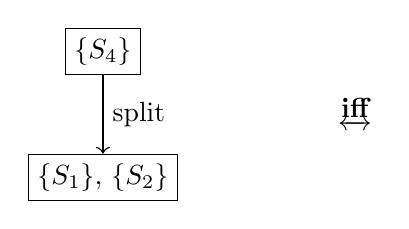
\begin{tikzpicture}[scale=0.8]
        \node (1) [draw, rectangle] {\{$S_4$\}};
        \node (2) [below=of 1, draw, rectangle] { \{$S_1$\}, \{$S_2$\}};
        \draw[->]  (1) to node [auto] {split} (2);
        \node (a) at (4,-1) {$\underleftrightarrow{\textbf{iff}}$};            % Label reject
      \end{tikzpicture}
    \end{scaletikzpicturetowidth}
    \caption{Initial token configuration $T_{A}$.}
    \label{fig:standard_1}
  \end{subfigure}
  \begin{subfigure}[b]{0.4\textwidth}
    \begin{scaletikzpicturetowidth}{\textwidth}
      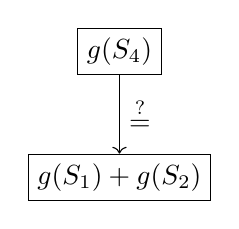
\begin{tikzpicture}[scale=0.8]
        \node (1) [draw, rectangle] {$g(S_4)$};
        \node (2) [below=of 1, draw, rectangle] { $g(S_1) + g(S_2)$};
        \draw[->]  (1) to node [auto] {$\stackrel{?}{=}$} (2);
      \end{tikzpicture}
    \end{scaletikzpicturetowidth}
    \caption{Target token configuration $T_{B}$.}
    \label{fig:standard_2}
  \end{subfigure}
  \caption{A Standard sliding token instance with initial and target labelled token configuration $T_{A}$ and $T_{B}$ respectively.}
  \label{fig:input_instance_standard}
\end{figure}

\end{example}




\chapter{Conclusions and Future Work}
Throughout this thesis, we have researched and analysed reconfiguration problems by starting with the Nondeterministic Constraint Logic
which seems to be the go-to reduction in order to prove $\PSPACE$-hardness results. More specifically, we focused on the alternative
formulation of NCL and detailed the $\PSPACE$-completeness result of the sliding token problem. We then showed that the labelled variant of the
SLIDING TOKEN problem is also $\PSPACE$-complete. This latter result was then used to establish the complexity result of the
$k$-move Subset sum reconfiguration problem for $k = 3$. Our contribution was to provide detailed explanatory examples and explications to complement
the proof of theorem \ref{theorem:3_move_theorem}.
All reconfiguration problems encountered during our journey to the completion of this thesis is summed in fig \ref{fig:conclusion}.

\begin{figure}[H]
    \begin{center}
        \begin{scaletikzpicturetowidth}{\textwidth}
            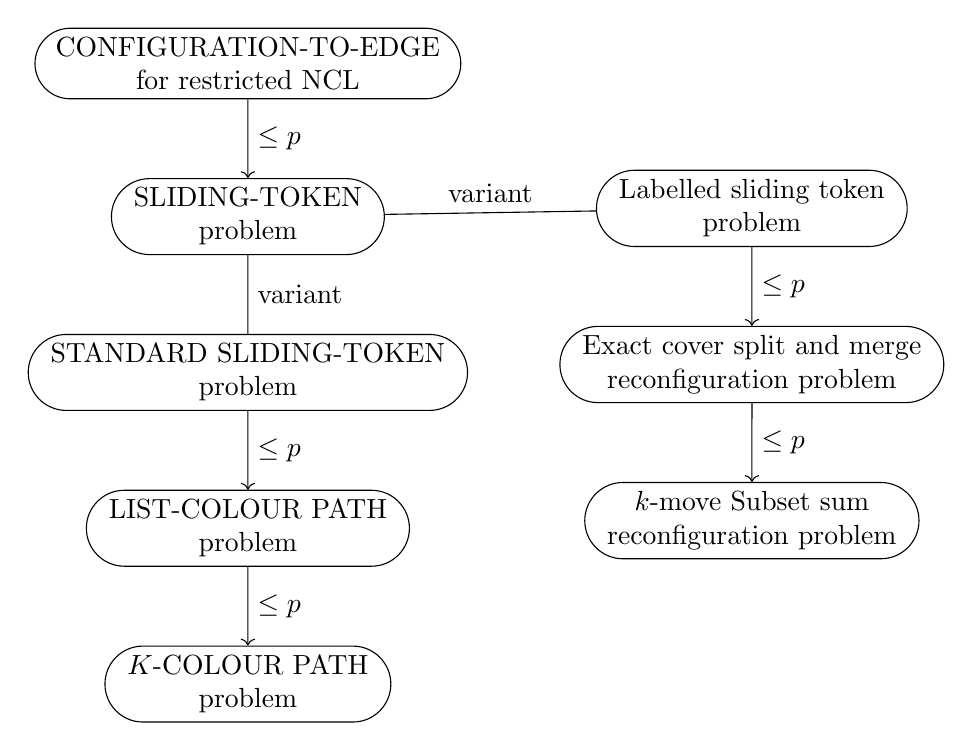
\begin{tikzpicture}[scale=0.8]
                \node (1) at (0,0) [draw, rounded rectangle, align=center] {CONFIGURATION-TO-EDGE\\for restricted NCL};
                \node (2)  [below=of 1, draw, rounded rectangle, align=center] {SLIDING-TOKEN\\problem};
                \node (3)  [below=of 2, draw, rounded rectangle, align=center] {STANDARD SLIDING-TOKEN\\problem};
                \node (4)  [below=of 3, draw, rounded rectangle, align=center] {LIST-COLOUR PATH\\problem};
                \node (5)  [below=of 4, draw, rounded rectangle, align=center] {$K$-COLOUR PATH\\problem};
                \node (6) at (8, -2.3) [draw, rounded rectangle, align=center] {Labelled sliding token\\problem};
                \node (7) [below=of 6, draw, rounded rectangle, align=center] {Exact cover split and merge\\ reconfiguration problem};
                \node (8) [below=of 7, draw, rounded rectangle, align=center] {$k$-move Subset sum\\reconfiguration problem};

                \draw[->]  (1) to node [auto] {$\leq{p}$} (2);
                \draw[-]  (2) to node [auto] {variant} (3);
                \draw[->]  (3) to node [auto] {$\leq{p}$} (4);
                \draw[->]  (4) to node [auto] {$\leq{p}$} (5);
                \draw[-]  (2) to node [auto] {variant} (6);
                \draw[->]  (6) to node [auto] {$\leq{p}$} (7);
                \draw[->]  (7) to node [auto] {$\leq{p}$} (8);

            \end{tikzpicture}
        \end{scaletikzpicturetowidth}
    \end{center}
    \caption{$\PSPACE$-complete problems encountered and their relationship.}\label{fig:conclusion}
\end{figure}

%\begin{figure}[H]
  \centering
  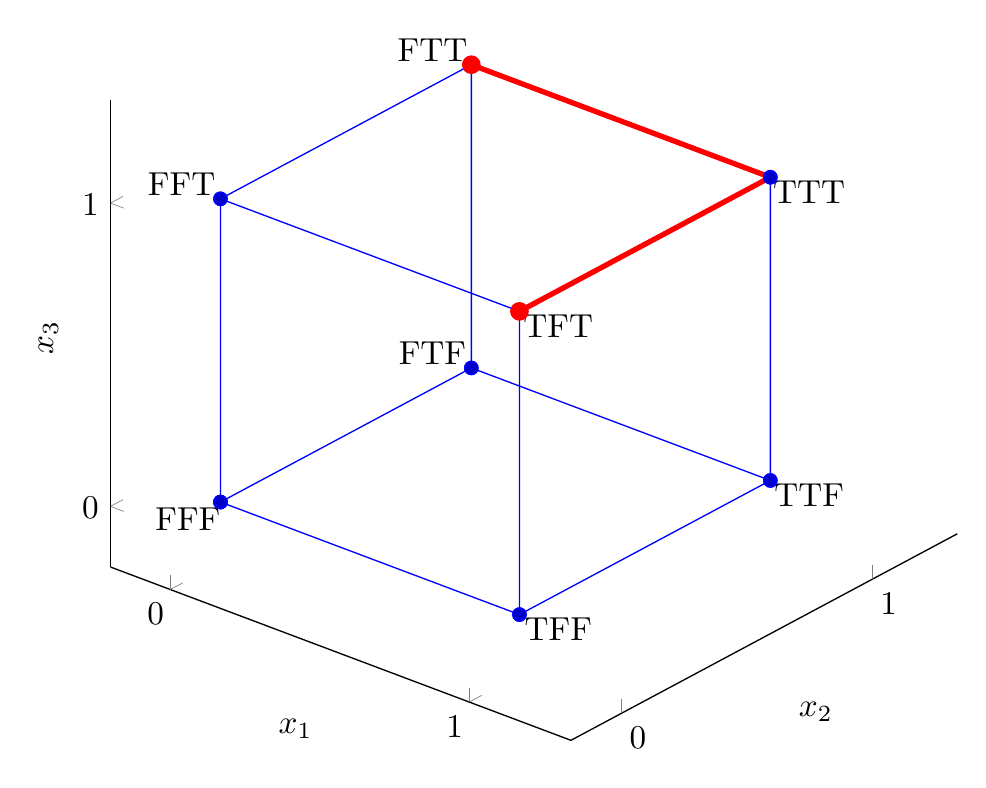
\begin{tikzpicture}[scale=1.2, x={({1}, {0})}]
    \begin{axis}[
      view/h=40,
      width=300pt,
      height=300pt,
      axis lines*=left,
      xmin=-0.2,xmax=1.2,
      ymin=-0.2,ymax=1.2,
      zmin=-0.2,zmax=1.2,
      enlargelimits=upper,
      xtick={0,1},
      ytick={0,1},
      ztick={0,1},
      xlabel={$x_1$},
      ylabel={$x_2$},
      zlabel={$x_3$}
    ]
      % pre-cube
      \addplot3 coordinates {(0,0,0) (0,1,0) (0,1,1) (0,0,1) (0,0,0)
        (0,0,1) (1,0,1) (1,0,0) (0,0,0) (1, 0, 0) (1,1,0) (0,1,0) (0,1,1) (1,1,1) (1,1,0) (1,1,1) (1,0,1)};

      \addplot3 [only marks, mark=*, fill=red, draw=red, ultra thick] coordinates {(0,1,1) (1,0,1)};

      \node (A) at (axis cs:0,-0.13,0) {FFF};
      \node (B) at (axis cs:-0.13,1,0) {FTF};
      \node (C) at (axis cs:-0.13,1,1) {FTT};
      \node (D) at (axis cs:-0.13,0,1) {FFT};
      \node (E) at (axis cs:1.13,0,1) {TFT};
      \node (F) at (axis cs:1.13,0,0) {TFF};
      \node (G) at (axis cs:1.13,1,0) {TTF};
      \node (H) at (axis cs:1.13,1,1) {TTT};

      % solution paths
      %\addplot3[draw=red, mark=none,ultra thick] coordinates {(0,1,1) (1,1,1) (1,1,0) (1,0,0) (0,0,0)};
      \addplot3[draw=red, mark=none,ultra thick] coordinates {(0,1,1) (1,1,1) (1,0,1)};
    \end{axis}
  \end{tikzpicture}
  \caption{Geometric visualisation of a given knapsack reconfiguration problem.}
  \label{fig:geo_1}
\end{figure}

\begin{figure}[H]
  \centering
  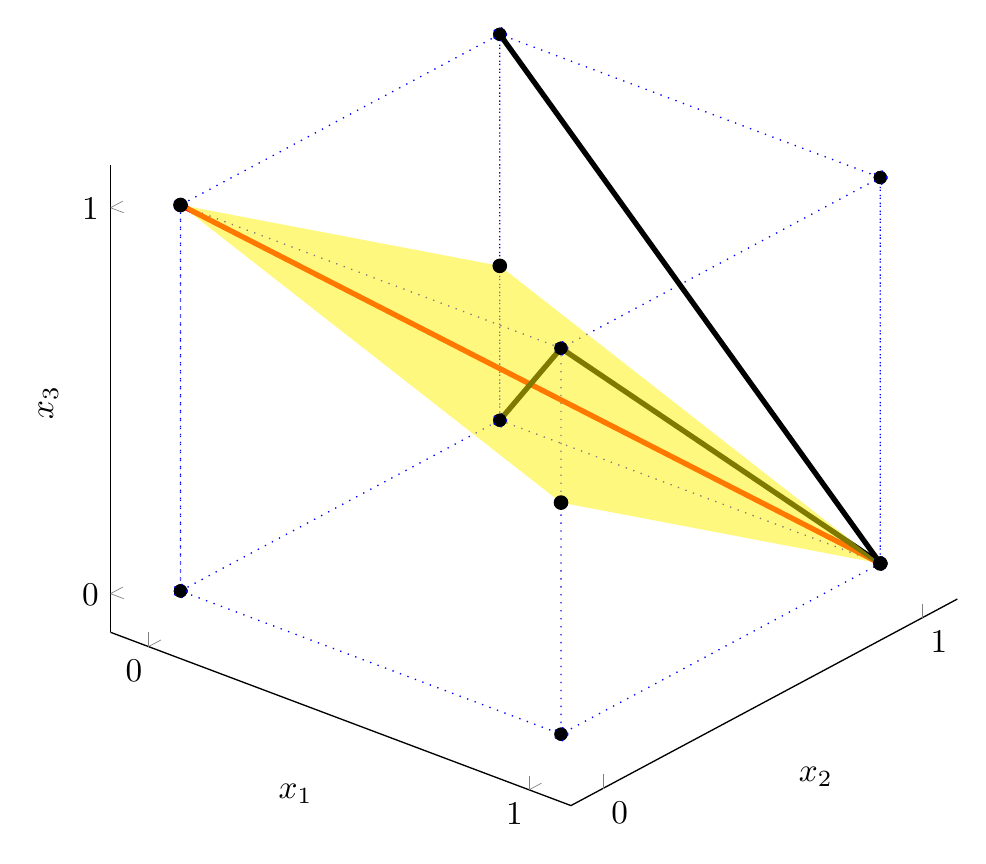
\begin{tikzpicture}[scale=1.2, x={({1}, {0})}]
    \begin{axis}[
      view/h=40,
      width=300pt,
      height=300pt,
      axis lines*=left,
      xmin=-0.1,xmax=1,
      ymin=-0.1,ymax=1,
      zmin=-0.1,zmax=1,
      enlargelimits=upper,
      xtick={0,1},
      ytick={0,1},
      ztick={0,1},
      xlabel={$x_1$},
      ylabel={$x_2$},
      zlabel={$x_3$}
    ]
      % pre-cube
      \addplot3[draw = blue, dotted, mark=*] coordinates {(0,0,0) (0,1,0) (0,1,1) (0,0,1) (0,0,0)
        (0,0,1) (1,0,1) (1,0,0) (0,0,0) (1, 0, 0) (1,1,0) (0,1,0) (0,1,1) (1,1,1) (1,1,0) (1,1,1) (1,0,1)};
      \addplot3[draw=red, ultra thick] coordinates {(0,0,1) (1,1,0)};
      \addplot3[fill=black, ultra thick] coordinates {(0,1,1) (1,1,0)};
      \addplot3[fill=black, ultra thick] coordinates {(1,0,1) (1,1,0)};
      \addplot3[fill=black, ultra thick] coordinates {(0,1,0) (1,0,1)};
      % upper
      \addplot3[draw = none, fill=yellow,fill opacity=0.5] coordinates {(1,0,3/5) (1,1,0) (0,1,2/5) (0,0,1) (1,0,3/5)};
      \addplot3 [only marks,mark=*] coordinates {(1,0,3/5) (1,1,0) (0,1,2/5) (0,0,1)};
      %\addplot3[mark=none,ultra thick] coordinates {(0,1,0) (1,1,0) (1,0,0) (1,0,1) (0,0,1)};
    \end{axis}
  \end{tikzpicture}
  \caption{Geometric visualisation of a given instance of the $3$-move SUBSET RECONFIGURATION problem.}
  \label{fig:geo_2}
\end{figure}


\begin{figure}[H]
  \centering
  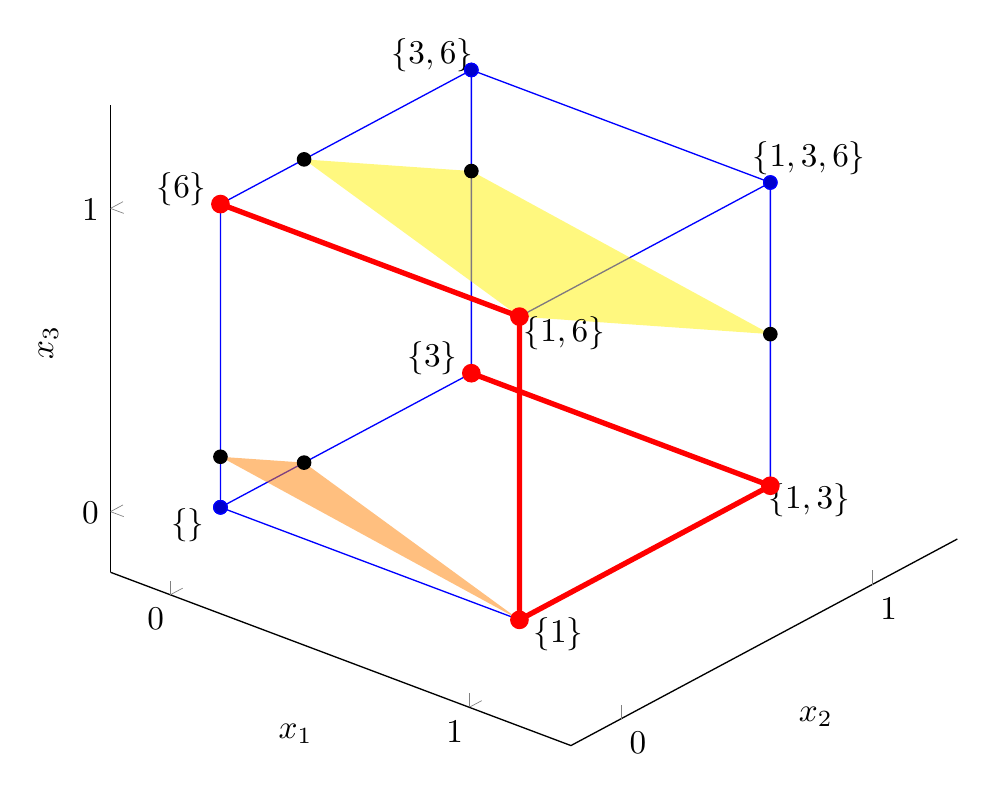
\begin{tikzpicture}[scale=1.2, x={({1}, {0})}]
    \begin{axis}[
      view/h=40,
      width=300pt,
      height=300pt,
      axis lines*=left,
      xmin=-0.2,xmax=1.2,
      ymin=-0.2,ymax=1.2,
      zmin=-0.2,zmax=1.2,
      enlargelimits=upper,
      xtick={0,1},
      ytick={0,1},
      ztick={0,1},
      xlabel={$x_1$},
      ylabel={$x_2$},
      zlabel={$x_3$}
    ]
      % pre-cube
      \addplot3 coordinates {(0,0,0) (0,1,0) (0,1,1) (0,0,1) (0,0,0)
        (0,0,1) (1,0,1) (1,0,0) (0,0,0) (1, 0, 0) (1,1,0) (0,1,0) (0,1,1) (1,1,1) (1,1,0) (1,1,1) (1,0,1)};
      % upper
      \addplot3[draw = none, fill=yellow,fill opacity=0.5] coordinates {(0,1,4/6) (1,1,1/2) (1,0,1)  (0,1/3,1) (0,1,4/6)};
      \addplot3 [only marks,mark=*] coordinates { (0,1,4/6) (1,1,1/2) (0,1/3,1)};

      %lower
      \addplot3[draw = none, fill=orange,fill opacity=0.5] coordinates {(1,0,0) (0,1/3,0) (0,0,1/6) (1,0,0)} ;
      \addplot3 [only marks,mark=*] coordinates { (1,0,0) (0,1/3,0) (0,0,1/6)};

      % solution paths
      \addplot3[draw=red, mark=none,ultra thick] coordinates {((0,0,1) (1,0,1) (1,0,0) (1,1,0) (0,1,0)};

      % initial and target confguration
      \addplot3 [only marks, mark=*, fill=red, draw=red, ultra thick] coordinates {(0,0,1) (1,0,1) (1,0,0) (1,1,0) (0,1,0)};

      \node (A) at (axis cs:0,-0.13,0) {$\{\}$};
      \node (B) at (axis cs:-0.13,1,0) {$\{3\}$};
      \node (C) at (axis cs:-0.13,1,1) {$\{3,6\}$};
      \node (D) at (axis cs:-0.13,0,1) {$\{6\}$};
      \node (E) at (axis cs:1.15,0,1) {$\{1,6\}$};
      \node (F) at (axis cs:1.13,0,0) {$\{1\}$};
      \node (G) at (axis cs:1.13,1,0) {$\{1,3\}$};
      \node (H) at (axis cs:1.13,1,1.13) {$\{1,3,6\}$};
    \end{axis}
  \end{tikzpicture}
  \caption{Geometric visualisation of a given knapsack reconfiguration problem.}
  \label{fig:geo_1}
\end{figure}



\begin{figure}[H]
  \centering
  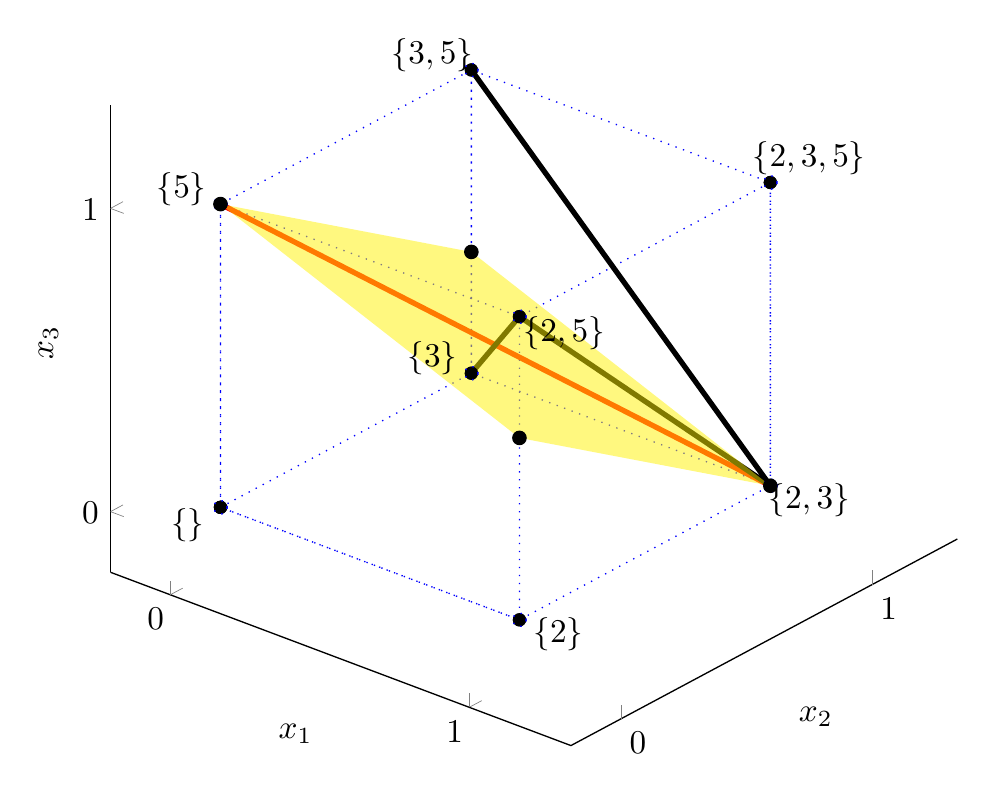
\begin{tikzpicture}[scale=1.2, x={({1}, {0})}]
    \begin{axis}[
      view/h=40,
      width=300pt,
      height=300pt,
      axis lines*=left,
      xmin=-0.2,xmax=1.2,
      ymin=-0.2,ymax=1.2,
      zmin=-0.2,zmax=1.2,
      enlargelimits=upper,
      xtick={0,1},
      ytick={0,1},
      ztick={0,1},
      xlabel={$x_1$},
      ylabel={$x_2$},
      zlabel={$x_3$}
    ]
      % pre-cube
      \addplot3[draw = blue, dotted, mark=*] coordinates {(0,0,0) (0,1,0) (0,1,1) (0,0,1) (0,0,0)
        (0,0,1) (1,0,1) (1,0,0) (0,0,0) (1, 0, 0) (1,1,0) (0,1,0) (0,1,1) (1,1,1) (1,1,0) (1,1,1) (1,0,1)};
      \addplot3[draw=red, ultra thick] coordinates {(0,0,1) (1,1,0)};
      \addplot3[fill=black, ultra thick] coordinates {(0,1,1) (1,1,0)};
      \addplot3[fill=black, ultra thick] coordinates {(1,0,1) (1,1,0)};
      \addplot3[fill=black, ultra thick] coordinates {(0,1,0) (1,0,1)};
      % upper
      \addplot3[draw = none, fill=yellow,fill opacity=0.5] coordinates {(1,0,3/5) (1,1,0) (0,1,2/5) (0,0,1) (1,0,3/5)};
      \addplot3 [only marks,mark=*] coordinates {(1,0,3/5) (1,1,0) (0,1,2/5) (0,0,1)};
      %\addplot3[mark=none,ultra thick] coordinates {(0,1,0) (1,1,0) (1,0,0) (1,0,1) (0,0,1)};

      \node (A) at (axis cs:0,-0.13,0) {$\{\}$};
      \node (B) at (axis cs:-0.13,1,0) {$\{3\}$};
      \node (C) at (axis cs:-0.13,1,1) {$\{3,5\}$};
      \node (D) at (axis cs:-0.13,0,1) {$\{5\}$};
      \node (E) at (axis cs:1.15,0,1) {$\{2,5\}$};
      \node (F) at (axis cs:1.13,0,0) {$\{2\}$};
      \node (G) at (axis cs:1.13,1,0) {$\{2,3\}$};
      \node (H) at (axis cs:1.13,1,1.13) {$\{2,3,5\}$};

    \end{axis}
  \end{tikzpicture}
  \caption{Geometric visualisation of a given instance of the $3$-move SUBSET RECONFIGURATION problem.}
  \label{fig:geo_2}
\end{figure}


\begin{figure}[H]
  \begin{center}
        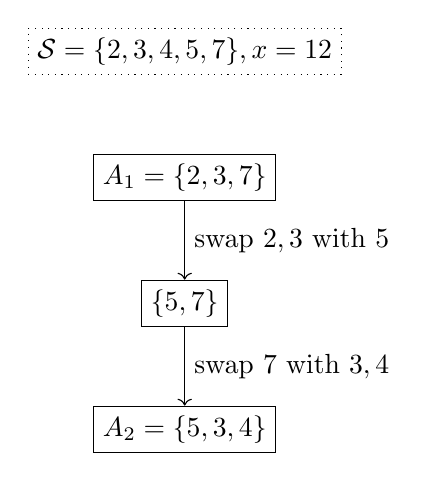
\begin{tikzpicture}[scale=1]
          \node (1) at (0,0) [draw, dotted, rectangle, align=center] {$\mathcal{S} = \{2, 3, 4, 5, 7\}, x = 12$};
          \node (2)  [below=of 1, draw, rectangle, align=center] {$A_1 = \{2, 3, 7\}$};
          \node (3)  [below=of 2, draw, rectangle, align=center] {$\{5, 7\}$};
          \node (4) [below=of 3, draw, rectangle, align=center] {$A_2 = \{5, 3, 4\}$};

          \draw[->]  (2) to node [auto] {swap $2, 3$ with $5$} (3);
          \draw[->]  (3) to node [auto] {swap $7$ with $3,4$} (4);
        \end{tikzpicture}
  \end{center}
  \caption{$\PSPACE$-complete problems encountered and their relationship.}\label{fig:conclusion}
\end{figure}


\begin{figure}[H]
  \begin{center}
        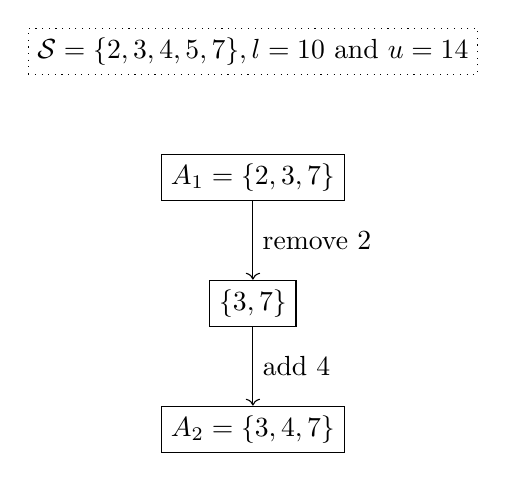
\begin{tikzpicture}[scale=1]
          \node (1) at (0,0) [draw, dotted, rectangle, align=center] {$\mathcal{S} = \{2, 3, 4, 5, 7\}, l = 10$ and $u = 14$};
          \node (2)  [below=of 1, draw, rectangle, align=center] {$A_1 = \{2, 3, 7\}$};
          \node (3)  [below=of 2, draw, rectangle, align=center] {$\{3, 7\}$};
          \node (4) [below=of 3, draw, rectangle, align=center] {$A_2 = \{3, 4, 7\}$};

          \draw[->]  (2) to node [auto] {remove $2$} (3);
          \draw[->]  (3) to node [auto] {add $4$} (4);
        \end{tikzpicture}
  \end{center}
  \caption{$\PSPACE$-complete problems encountered and their relationship.}\label{fig:conclusion}
\end{figure}



\begin{figure}[H]
  \centering
  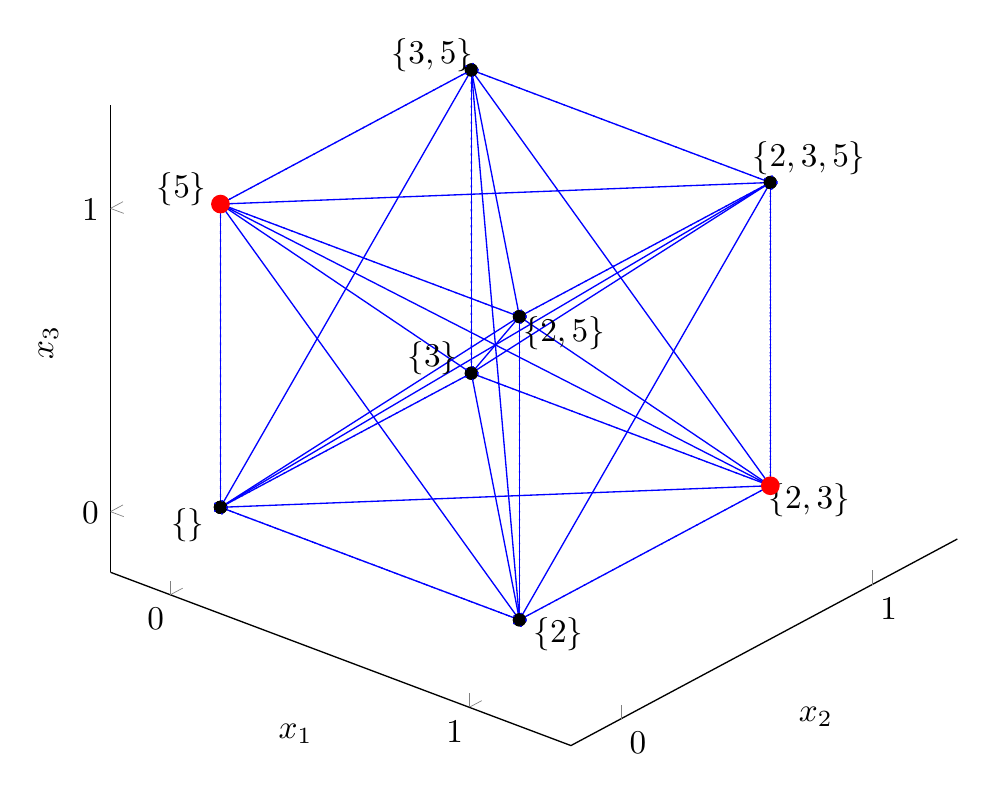
\begin{tikzpicture}[scale=1.2, x={({1}, {0})}]
    \begin{axis}[
      view/h=40,
      width=300pt,
      height=300pt,
      axis lines*=left,
      xmin=-0.2,xmax=1.2,
      ymin=-0.2,ymax=1.2,
      zmin=-0.2,zmax=1.2,
      enlargelimits=upper,
      xtick={0,1},
      ytick={0,1},
      ztick={0,1},
      xlabel={$x_1$},
      ylabel={$x_2$},
      zlabel={$x_3$}
    ]
      % pre-cube
      \addplot3[draw = blue, dotted, mark=*] coordinates {(0,0,0) (0,1,0) (0,1,1) (0,0,1) (0,0,0)
        (0,0,1) (1,0,1) (1,0,0) (0,0,0) (1, 0, 0) (1,1,0) (0,1,0) (0,1,1) (1,1,1) (1,1,0) (1,1,1) (1,0,1)};


      % initial and target confguration
      \addplot3 [only marks, mark=*, fill=red, draw=red, ultra thick] coordinates {(0,0,1) (1,1,0)};

      \addplot3[draw=blue] coordinates {(0,0,0) (0,1,0)};
      \addplot3[draw=blue] coordinates {(0,0,0) (0,1,1)};
      \addplot3[draw=blue] coordinates {(0,0,0) (0,0,1)};
      \addplot3[draw=blue] coordinates {(0,0,0) (1,0,1)};
      \addplot3[draw=blue] coordinates {(0,0,0) (1,0,0)};
      \addplot3[draw=blue] coordinates {(0,0,0) (1,1,0)};
      \addplot3[draw=blue] coordinates {(0,0,0) (1,1,1)};

      \addplot3[draw=blue] coordinates {(0,1,0) (0,1,1)};
      \addplot3[draw=blue] coordinates {(0,1,0) (0,0,1)};
      \addplot3[draw=blue] coordinates {(0,1,0) (1,0,1)};
      \addplot3[draw=blue] coordinates {(0,1,0) (1,0,0)};
      \addplot3[draw=blue] coordinates {(0,1,0) (1,1,0)};
      \addplot3[draw=blue] coordinates {(0,1,0) (1,1,1)};

      \addplot3[draw=blue] coordinates {(0,1,1) (0,0,1)};
      \addplot3[draw=blue] coordinates {(0,1,1) (1,0,1)};
      \addplot3[draw=blue] coordinates {(0,1,1) (1,0,0)};
      \addplot3[draw=blue] coordinates {(0,1,1) (1,1,0)};
      \addplot3[draw=blue] coordinates {(0,1,1) (1,1,1)};


      \addplot3[draw=blue] coordinates {(0,0,1) (1,0,0)};
      \addplot3[draw=blue] coordinates {(0,0,1) (1,1,0)};
      \addplot3[draw=blue] coordinates {(0,0,1) (1,1,1)};

      \addplot3[draw=blue] coordinates {(1,0,1) (0,0,1)};
      \addplot3[draw=blue] coordinates {(1,0,1) (1,0,0)};
      \addplot3[draw=blue] coordinates {(1,0,1) (1,1,0)};
      \addplot3[draw=blue] coordinates {(1,0,1) (1,1,1)};

      \addplot3[draw=blue] coordinates {(1,0,0) (1,1,0)};
      \addplot3[draw=blue] coordinates {(1,0,0) (1,1,1)};

      \addplot3[draw=blue] coordinates {(1,1,0) (1,1,1)};



      \node (A) at (axis cs:0,-0.13,0) {$\{\}$};        % 000
      \node (B) at (axis cs:-0.13,1,0) {$\{3\}$};       % 010
      \node (C) at (axis cs:-0.13,1,1) {$\{3,5\}$};     % 011
      \node (D) at (axis cs:-0.13,0,1) {$\{5\}$};       % 001
      \node (E) at (axis cs:1.15,0,1) {$\{2,5\}$};      % 101
      \node (F) at (axis cs:1.13,0,0) {$\{2\}$};        % 100
      \node (G) at (axis cs:1.13,1,0) {$\{2,3\}$};      % 110
      \node (H) at (axis cs:1.13,1,1.13) {$\{2,3,5\}$}; % 111

    \end{axis}
  \end{tikzpicture}
  \caption{Geometric visualisation of a given instance of the $3$-move SUBSET RECONFIGURATION problem.}
  \label{fig:geo_2}
\end{figure}


\begin{figure}[H]
  \centering
  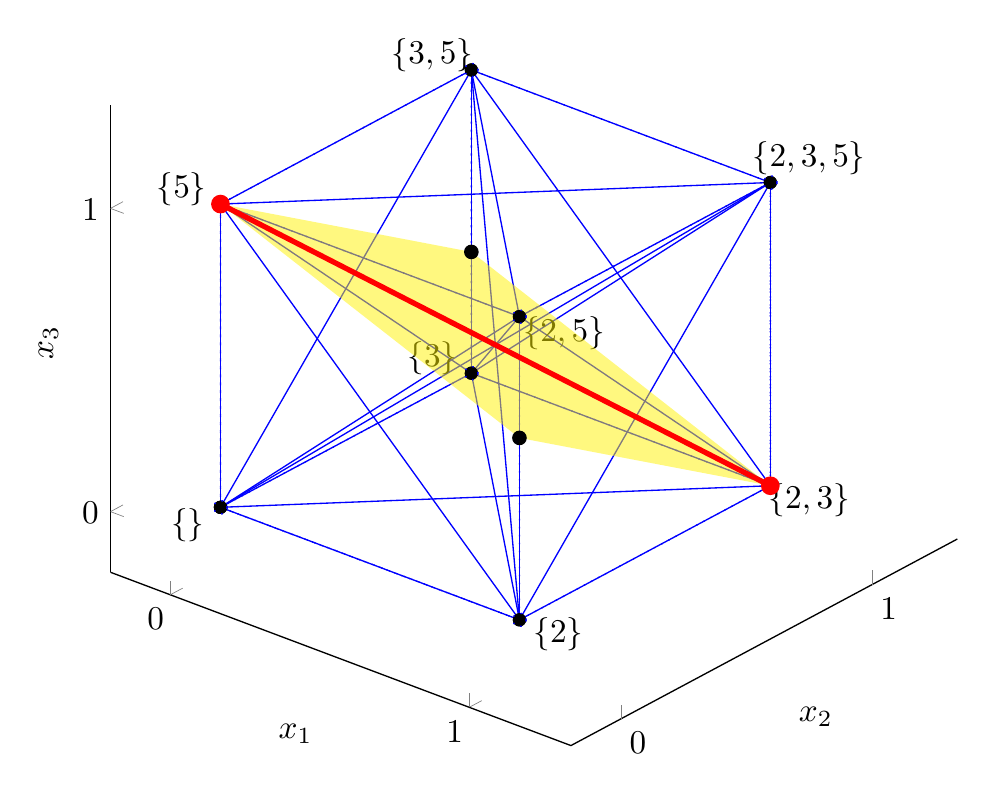
\begin{tikzpicture}[scale=1.2, x={({1}, {0})}]
    \begin{axis}[
      view/h=40,
      width=300pt,
      height=300pt,
      axis lines*=left,
      xmin=-0.2,xmax=1.2,
      ymin=-0.2,ymax=1.2,
      zmin=-0.2,zmax=1.2,
      enlargelimits=upper,
      xtick={0,1},
      ytick={0,1},
      ztick={0,1},
      xlabel={$x_1$},
      ylabel={$x_2$},
      zlabel={$x_3$}
    ]
      % pre-cube
      \addplot3[draw = blue, dotted, mark=*] coordinates {(0,0,0) (0,1,0) (0,1,1) (0,0,1) (0,0,0)
        (0,0,1) (1,0,1) (1,0,0) (0,0,0) (1, 0, 0) (1,1,0) (0,1,0) (0,1,1) (1,1,1) (1,1,0) (1,1,1) (1,0,1)};

      \addplot3[draw=blue] coordinates {(0,0,0) (0,1,0)};
      \addplot3[draw=blue] coordinates {(0,0,0) (0,1,1)};
      \addplot3[draw=blue] coordinates {(0,0,0) (0,0,1)};
      \addplot3[draw=blue] coordinates {(0,0,0) (1,0,1)};
      \addplot3[draw=blue] coordinates {(0,0,0) (1,0,0)};
      \addplot3[draw=blue] coordinates {(0,0,0) (1,1,0)};
      \addplot3[draw=blue] coordinates {(0,0,0) (1,1,1)};

      \addplot3[draw=blue] coordinates {(0,1,0) (0,1,1)};
      \addplot3[draw=blue] coordinates {(0,1,0) (0,0,1)};
      \addplot3[draw=blue] coordinates {(0,1,0) (1,0,1)};
      \addplot3[draw=blue] coordinates {(0,1,0) (1,0,0)};
      \addplot3[draw=blue] coordinates {(0,1,0) (1,1,0)};
      \addplot3[draw=blue] coordinates {(0,1,0) (1,1,1)};

      \addplot3[draw=blue] coordinates {(0,1,1) (0,0,1)};
      \addplot3[draw=blue] coordinates {(0,1,1) (1,0,1)};
      \addplot3[draw=blue] coordinates {(0,1,1) (1,0,0)};
      \addplot3[draw=blue] coordinates {(0,1,1) (1,1,0)};
      \addplot3[draw=blue] coordinates {(0,1,1) (1,1,1)};


      \addplot3[draw=blue] coordinates {(0,0,1) (1,0,0)};
      \addplot3[draw=blue] coordinates {(0,0,1) (1,1,0)};
      \addplot3[draw=blue] coordinates {(0,0,1) (1,1,1)};

      \addplot3[draw=blue] coordinates {(1,0,1) (0,0,1)};
      \addplot3[draw=blue] coordinates {(1,0,1) (1,0,0)};
      \addplot3[draw=blue] coordinates {(1,0,1) (1,1,0)};
      \addplot3[draw=blue] coordinates {(1,0,1) (1,1,1)};

      \addplot3[draw=blue] coordinates {(1,0,0) (1,1,0)};
      \addplot3[draw=blue] coordinates {(1,0,0) (1,1,1)};

      \addplot3[draw=blue] coordinates {(1,1,0) (1,1,1)};

      \node (A) at (axis cs:0,-0.13,0) {$\{\}$};        % 000
      \node (B) at (axis cs:-0.13,1,0) {$\{3\}$};       % 010
      \node (C) at (axis cs:-0.13,1,1) {$\{3,5\}$};     % 011
      \node (D) at (axis cs:-0.13,0,1) {$\{5\}$};       % 001
      \node (E) at (axis cs:1.15,0,1) {$\{2,5\}$};      % 101
      \node (F) at (axis cs:1.13,0,0) {$\{2\}$};        % 100
      \node (G) at (axis cs:1.13,1,0) {$\{2,3\}$};      % 110
      \node (H) at (axis cs:1.13,1,1.13) {$\{2,3,5\}$}; % 111

      % upper
      \addplot3[draw = none, fill=yellow,fill opacity=0.5] coordinates {(1,0,3/5) (1,1,0) (0,1,2/5) (0,0,1) (1,0,3/5)};
      \addplot3 [only marks,mark=*] coordinates {(1,0,3/5) (1,1,0) (0,1,2/5) (0,0,1)};

      \addplot3[draw=red, ultra thick, mark=none] coordinates {(0,0,1) (1,1,0)};

      % initial and target confguration
      \addplot3 [only marks, mark=*, fill=red, draw=red, ultra thick] coordinates {(0,0,1) (1,1,0)};

    \end{axis}
  \end{tikzpicture}
  \caption{Geometric visualisation of a given instance of the $3$-move SUBSET RECONFIGURATION problem.}
  \label{fig:geo_2}
\end{figure}




%----------------------------------------------------------------------------------------
%	THESIS CONTENT - APPENDICES
%----------------------------------------------------------------------------------------

    \appendix % Cue to tell LaTeX that the following "chapters" are Appendices

% Include the appendices of the thesis as separate files from the Appendices folder
% Uncomment the lines as you write the Appendices

%% Appendix A

\chapter{Frequently Asked Questions} % Main appendix title

\label{AppendixA} % For referencing this appendix elsewhere, use \ref{AppendixA}

\section{How do I change the labelleds of links?}

The  of links can be changed to your liking using:

{\small\verb!\hypersetup{url=red}!}, or

{\small\verb!\hypersetup{cite=green}!}, or

{\small\verb!\hypersetup{all=blue}!}.

\noindent If you want to completely hide the links, you can use:

{\small\verb!\hypersetup{alls=.}!}, or even better:

{\small\verb!\hypersetup{hidelinks}!}.

\noindent If you want to have obvious links in the PDF but not the printed text, use:

{\small\verb!\hypersetup{links=false}!}.

%\include{Appendices/AppendixB}
%\include{Appendices/AppendixC}

%----------------------------------------------------------------------------------------
%	BIBLIOGRAPHY
%----------------------------------------------------------------------------------------
    \nocite{*}
    \bibliography{main}
    \bibliographystyle{plain}

\end{document}
